\RequirePackage{lineno}
\documentclass[12pt,a4paper]{article}
\usepackage[T1]{fontenc}
\usepackage{graphicx}
\usepackage{hyperref}
\usepackage{caption}
\usepackage{mathptmx}
\usepackage[absolute,overlay]{textpos}
\usepackage{fancybox}
\usepackage{multirow}
\usepackage[dvipsnames,table,xcdraw]{xcolor}
\usepackage{amsmath, amsthm, amssymb,amsfonts}
\usepackage{float}
\usepackage{fullpage}
\usepackage{units}
\usepackage{xspace}
\usepackage{caption}
\usepackage{subcaption}
\usepackage{array}
\usepackage{tikz}
\usepackage{placeins}  % for FloatBarrier
\usepackage[nottoc,notlot,notlof]{tocbibind}
\usetikzlibrary{decorations.pathreplacing}
\usepackage{authblk} % To add authors' affiliations

%%% Code to enter C++ code
\usepackage{listings}
\linenumbers % Include line numbers
\lstset{language=C++,
        basicstyle=\ttfamily,
        keywordstyle=\color{blue}\ttfamily,
        stringstyle=\color{red}\ttfamily,
        commentstyle=\color{green}\ttfamily,
        morecomment=[l][\color{magenta}]{\#}
}

\usepackage{hyperref}
\hypersetup{
    colorlinks,
    citecolor=blue!90!black,
    filecolor=black,
    linkcolor=blue!50!black,
    urlcolor=blue!50!black
}

\author[1]{Róbert Králik}
\affil[1]{University of Sussex, Brighton, UK}
\title{\textbf{NOvA Test Beam detector calibration\\ \vspace*{5mm}
\Large{Technical Note}}}
\date{\today}

\begin{document}
\maketitle
\thispagestyle{empty} % Remove page number from title page
\begin{abstract}
The NOvA Test Beam detector calibration uses the same calibration procedure as the standard NOvA detectors. The main aim is to remove differences in energy deposition within the detector and to provide an absolute energy scale from collected charge to physical energy units. This allows for a direct comparison of the deposited energy in the Test Beam detector with the standard NOvA detectors. On top of that, the unique qualities of Test Beam allow us to use the Test Beam calibration to validate the calibration process and possibly to provide a simulation-independent absolute energy scale.
\end{abstract}
\newpage

\thispagestyle{empty} % Remove page number from ToC
\tableofcontents
\newpage
\pagenumbering{arabic} % Start pagenumbering from here

\section{Introduction}

The NOvA Test Beam experiment aims to improve NOvA's sensitivity to the neutrino oscillation parameters by improving our understanding of particle interactions and energy deposition in the NOvA detectors, with the hope of reducing the total systematic uncertainty by about 10\% \cite{NOVA-doc-33012}.
 
Specifically, Test Beam allows us to study the response of tagged single particles as a function of their measured energies and compare it to the simulated prediction. It also enables us to determine the energy resolution and the absolute energy scale of these particles. Additionally, we are able to compare the response of beam and cosmic ray muons, to study fibre attenuation, or to validate the entire NOvA calibration process. Test Beam detector was also equipped with a combination of near and far detector readout electronics and filled with a variety of NOvA scintillator oils, which makes it possible to make a comparison of their responses \cite{NOVA-doc-15750}.

All the aforementioned benefits of running the NOvA Test Beam experiment require, or benefit from, the Test Beam detector calibration.

The Test Beam detector calibration was first pioneered by Kevin Moulder who adapted the NOvA calibration codebase for Test Beam and tested it on period 1 Test Beam data \cite{NOVA-doc-42700}. This was followed by Anna Hall who improved it and got the first usable calibration of the Test Beam detector based on the period 2 data \cite{NOVA-doc-50786}. Lastly, Rober Kralik took over and finished the Test Beam calibration with help from Randeeth Dasanayaka with all Test Beam data and a new simulation in 2023 \cite{NOVA-doc-59024}.

%Only considering improvement in the calibration systematic uncertainty, the NOvA Test Beam program can reduce the overal systematic uncertainty for the main NOvA measurements by about 10\% [docdb:33012] (talk also contains a list of other talks on impact of TB in different NOvA areas). For DeltaM2: By increasing exposure, total syst. error decreases by (+) 18.5% (-) 25%; By increasing exposure and reducing calib systs., total syst. error decreases by: (+) 26% (-) 32%; Difference between the above (reducing calib systs. with large exposure): (+) 9.6% (-) 9.4%. For sin2Th23: Difference by reducing calib syst.: (+) 10.8% (-) 9.4%.
%Statement: “The NOvA Test Beam will improve the total systema6c error on the final measurement of the oscilla6on parameters Dm232 and sin2Th23 by 10% from reduc6on of calibra6on systema6cs alone. Further, NOvA analyses will benefit from the detailed understanding of detector response to hadronic, electromagne6c, and muon energy provided by the Test Beam, which will be essen6al to solidify understanding of systema6cs, uncover poten6ally new uncertain6es, tune the simula6on modeling, and improve reconstruc6on and PID algorithms.”
%Potential Test Beam impacts: Check modeling of hadronic interacOons in detector (check GEANT systemaOcs), Using Test Beam data as “single-parOcle MC” to train CVN prong-like algorithms, GeneraOve Adversarial Networks for MC improvements using Test Beam data, Check ND calibraOon procedure to try and understand causes of 3-5% discrepancy between data and MC for muons and protons  (Birks suppression measurement), Data/MC comparisons of observed and clustered visible energy to improve dead material correcOons and energy esOmators, Acquire beier understanding of gain and photon transport, aienuaOon, Cherenkov light modeling, [DifferenOal] charged pion and proton cross secOon measurements would be extremely useful!, CalibraOng with test beam muons vs. cosmic muons (differences between horizontal vs. verOcal muons? - possibly shed “light” on the calib shape uncertainty), Study path length inside cell, take beam data with non-orthogonal incidence, Cross-check pi0 invariant mass reconstrucOon and Michel tagging efficiency/spectra, Use neutron source to study modeling of neutron capture (I don't think this was done in the end...), Playing with different GEANT physics lists to boost our confidence in the MC (pions? neutrons?)

%[docdb:15750 - NOvA Test Beam task force report]: The test beam program was included in the NOvA proposal [1] and was considered as an essential part of the experiment since its inception. Primary goals are oriented toward measurements of detector response to different particles with a range of momenta most relevant to NOvA beam physics studies, establishing of the absolute and relative energy scale of both NOvA detectors, and validating detailed and fast detector simulations code. [List all possible desired studies with Test Beam copied below] Two 31-layer 2 × 2 blocks, with approximate dimensions of 2.6 × 2.6 × 4 m3 were produced at the Minnesota factory before its shutdown (as a comparison, the 3 × 3 NOvA ND has 6 × 32 layers). In addition, 96 1 × 1 layers, with approximate total dimensions of 1.3 × 1.3 × 6.2 m3 were produced. Both 2 × 2 blocks and all the 1 × 1 layers were leak-tested. The 2 × 2 blocks are currently stored at the MINOS surface building, while the 1 × 1 layers are stored at the CDF building(?). The proposed detector to be deployed for the test beam run consists of the two 2 × 2 blocks. The NDOS decommissioning yielded 25000 gallons of scintillator. Since storage available is limited to 12000 gallons, it was decided to blend most of the 5000 gallons of existing ND/FD scintillator with the NDOS scintillator. 200 gallons of ND/FD scintillator, which has a slightly higher photon yield, are reserved for special studies. We also plan to reuse the NDOS secondary containment tub to provide oil+scintillator containment in case the test beam detector undergoes a catastrophic structural failure. Based on MINERvA’s experience, it is anticipated that two months of data taking would provide the necessary samples to carry out the test beam objectives.

%Also use information from:
%\begin{itemize}
%\item NOvA Test Beam Technical Statement of Work
%\item NOvA Test Beam program (paper for DOE) [docdb:25074]
%\item NOvA Test Beam task force report [docdb:15750]
%\item Overview presentation of NOvA Test Beam [docdb:20495]
%\item Test Beam support document [docdb:22172]
%\item NOvA Test Beam program proceedings [docdb:55808]
%\end{itemize}

%%%%%%%%%%%%%%%%%%%%%%%%%%%%%%%%%%%%%%%%%%%%%%%%%%%%%%%%%%%%%%%%%%%%%%%%%%%%%%%
%%%%%%%%%%%%%%%%%%%%%%%%%%%%%%%%%%%%%%%%%%%%%%%%%%%%%%%%%%%%%%%%%%%%%%%%%%%%%%%
%%%
%%%                       Test Beam detector description
%%%
%%%%%%%%%%%%%%%%%%%%%%%%%%%%%%%%%%%%%%%%%%%%%%%%%%%%%%%%%%%%%%%%%%%%%%%%%%%%%%%
\section{Overview of the Test Beam detector}\label{secTBDetector}
%What is Test Beam, how does the detector and beamline look like.
%Placed in MC7b together with a beamline instrumentation (no need to describe beamline).

The NOvA Test Beam detector is a scaled down version of the near and far detectors shown on Fig. \ref{figTBDetector}. It is placed in the MC7b enclosure of the Fermilab Test Beam Facility in the path of the MCenter beamline with a variety of beamline detectors to measure and identify a range of particles with various momenta \cite{NOVA-doc-22172-v2}.

\begin{figure}[!ht]
\centering
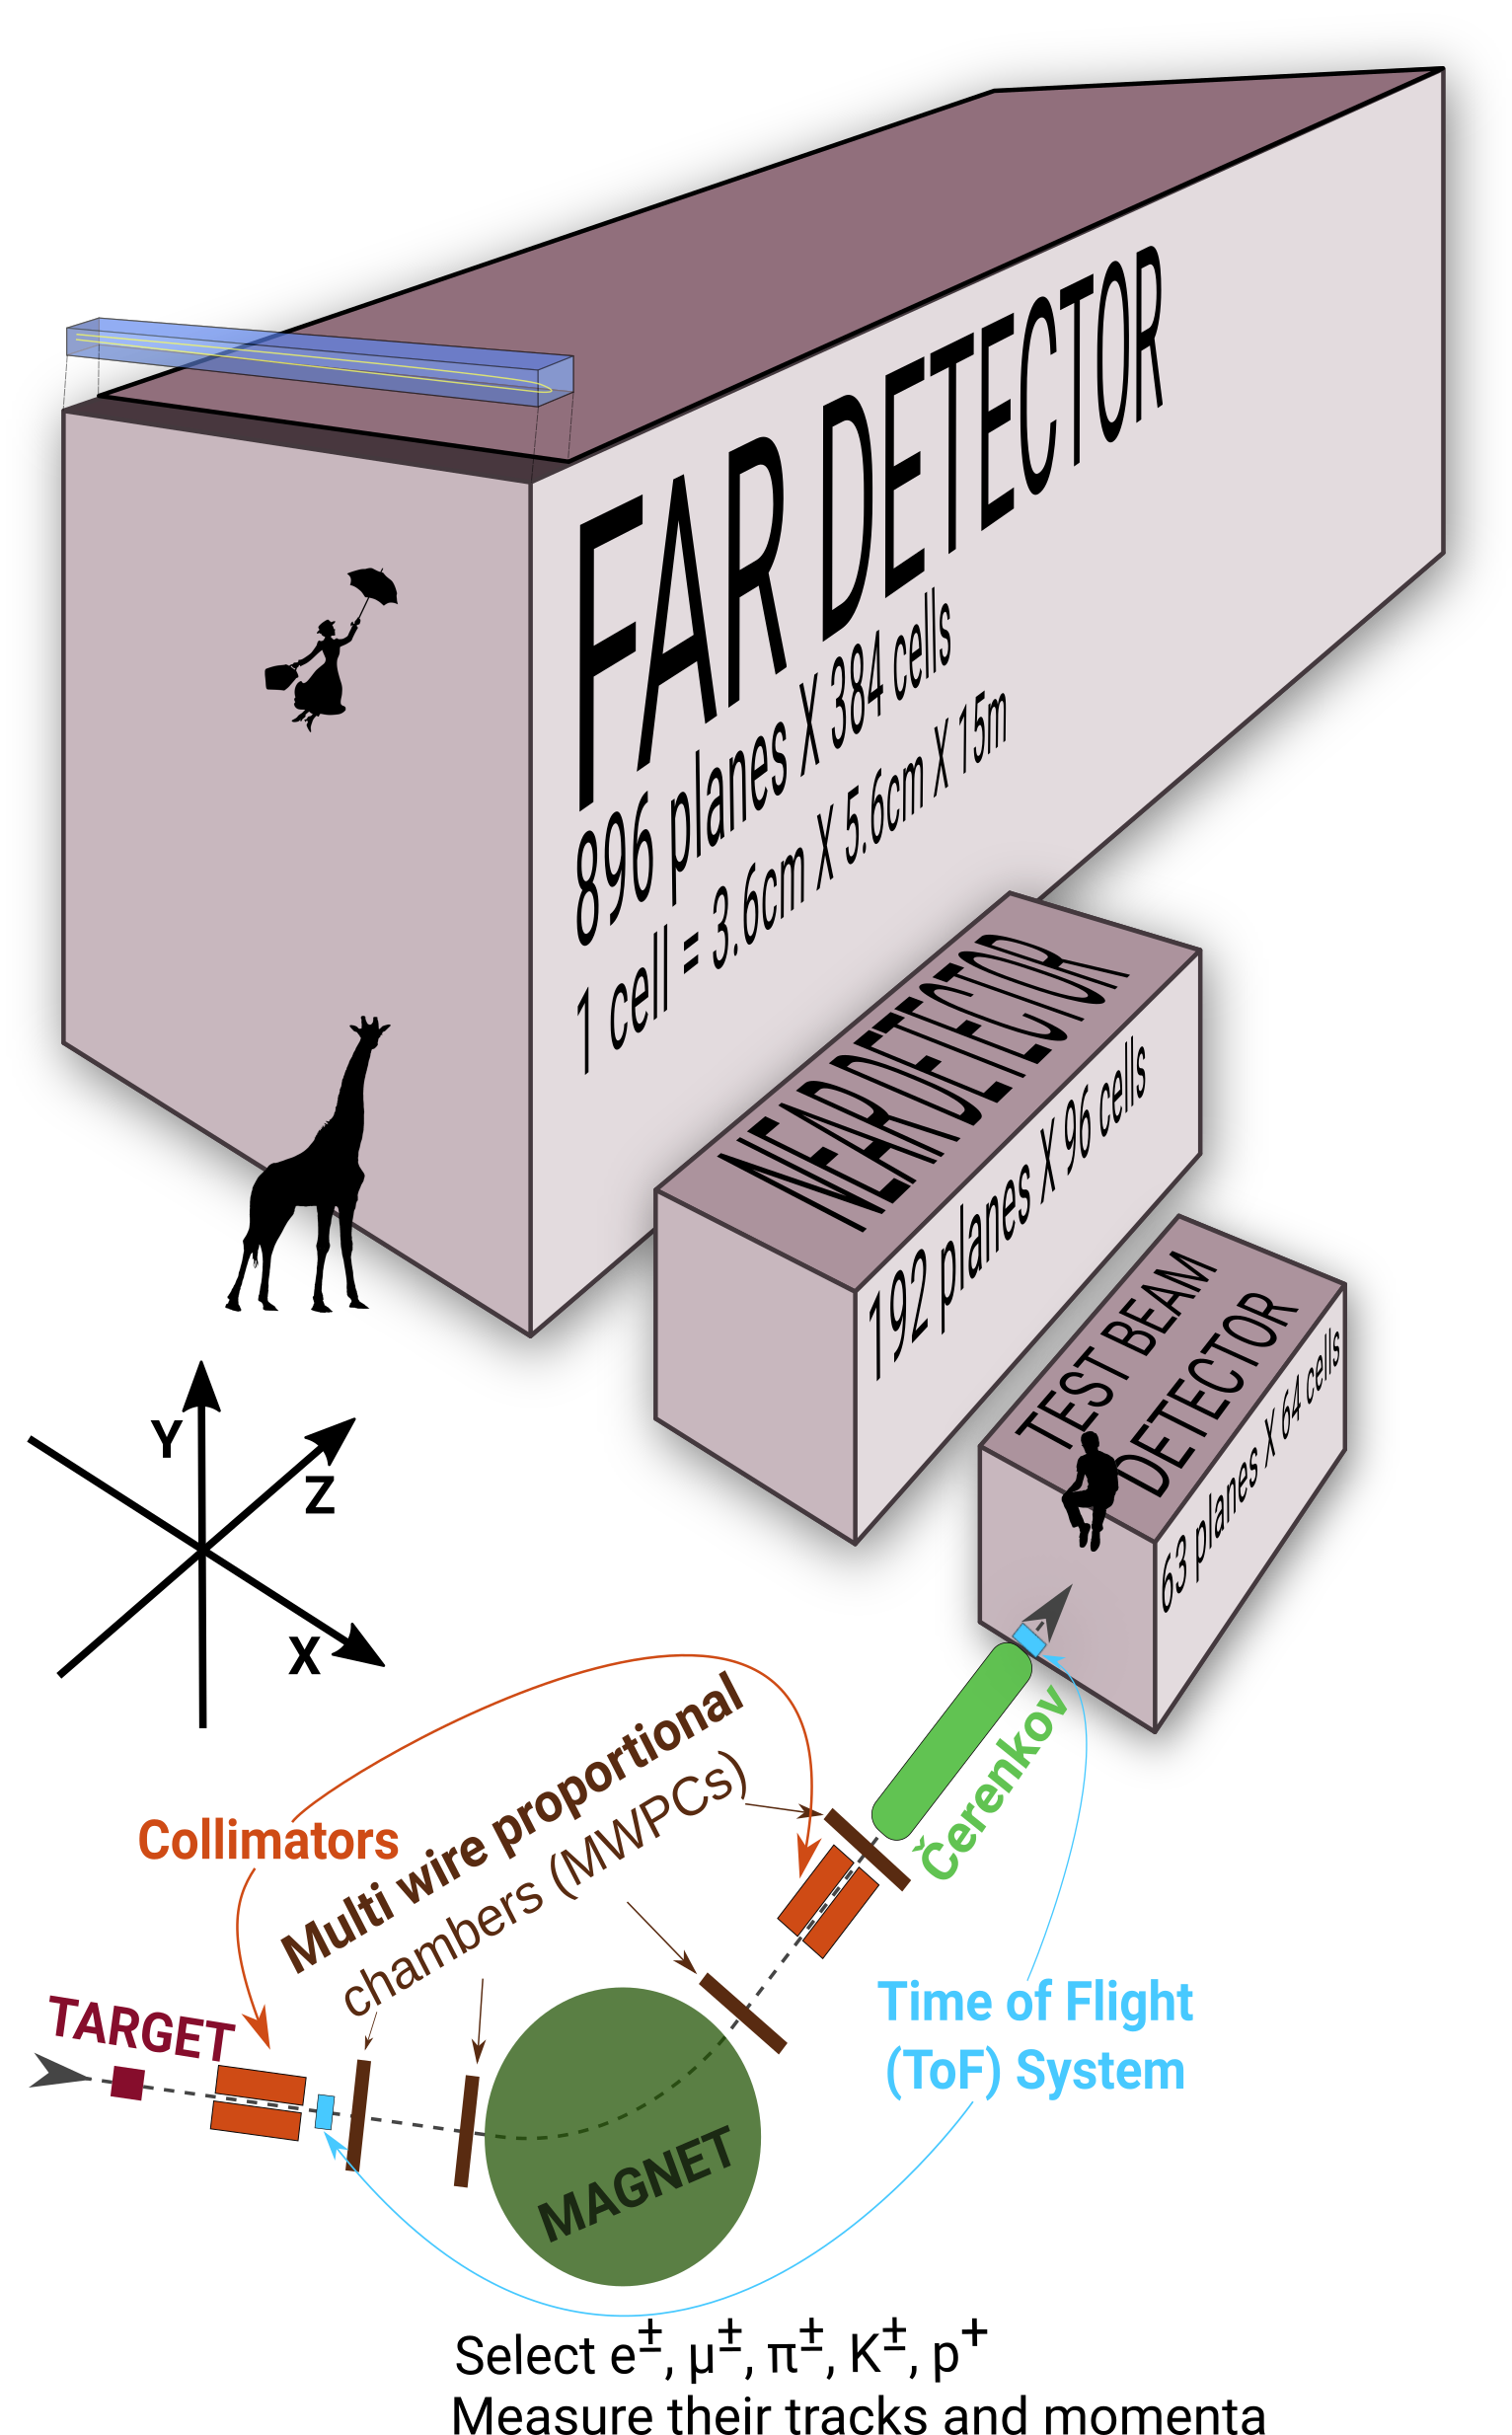
\includegraphics[width=.7\textwidth]{Plots/TestBeamDetectorWithArrows.png}
\caption{Comparison of Test Beam detector scale to the Near and Far NOvA detectors (and a man, giraffe, or Mary Poppins). Also shown are the Test Beam beamline detectors and components (not to scale), with arrows showing the direction of the beam. The three black arrows show the orientation of the detector coordinate system.}
\label{figTBDetector}
\end{figure}

%Should I aslo talk about the beam halo? Could that have an influence on the calibration? Maybe it's the peaks in the cosz distribution?

The Test Beam detector started with commissioning runs in June 2019 and ran, with an exception of regular summer shutdowns, until July 2022, after which it was decommissioned. The Test Beam data periods are:
\begin{table}[!ht]
\centering
\def\arraystretch{1.4}
\begin{tabular}{l@{\hskip 1in}lcl}
Period 1 & June $3^{\textsf{rd}}$ 2019 & - & July $6^{\textsf{th}}$ 2019\\
Period 2 & December $5^{\textsf{th}}$ 2019 & - & March $20^{\textsf{th}}$ 2020\\
Period 3 & January $12^{\textsf{th}}$ 2021 & - & June $27^{\textsf{th}}$ 2021\\
Period 4 & November $30^{\textsf{th}}$ 2021 & - & July $10^{\textsf{th}}$ 2022
\end{tabular}
\caption{Test Beam detector data taking periods.}
\label{tabTestBeamPeriods}
\end{table}

Majority of the Test Beam detector and its instrumentation is identical to the other NOvA detectors, with a few exceptions that could have an impact on the calibration. We are going to identify and discuss these differences in this section.

%[docdb:15750 - NOvA Test Beam task force report]: The test beam program was included in the NOvA proposal [1] and was considered as an essential part of the experiment since its inception. The main tangible result of these initial plans and later discussions was a production of special small extrusion modules, made at the end of the modules production stage, as possible components of a future test beam detector. In fact, this production followed and was based on initial simulations of a possible test beam experiment [5].

\subsubsection*{General parameters}
The NOvA Test Beam detector consists of two 31-plane blocks, each beginning and ending with a vertical plane, with an additional horizontal plane glued in-between them to preserve the alternating pattern \cite{NOVA-doc-29543}. Each plane consists of 2 modules side-by-side, both made up of 32 cells. Each cell is $2.6\,\unit{m}$ long with an inner (without the PVC) depth and width of $5.9\,\unit{cm}$ and $3.8\,\unit{cm}$ respectively, same as for the other NOvA detectors. This brings the final dimensions of the Test Beam detector to 63 planes $\times$ 64 cells, or $2.6\times 2.6\times 4.1\,\unit{m^3}$.

The 63 planes are numbered from 0 to 62, with even numbers corresponding to vertical planes and odd numbers to horizontal planes. Cells are numbered 0 to 63, going from bottom to top for horizontal planes and left to right, when facing the front of the detector, for vertical planes.

The detector coordinate system is illustrated on Fig. \ref{figTBDetector}. It is centred with $\left(0,0,0\right)$ in the centre of the first plane \cite{NOVA-doc-58388}. The x axis runs left to right when facing the front of the detector, y axis bottom to top, and z axis goes along the beam direction from front to the back of the detector. Position within each cell ($w$) is aligned with the x (y) axis for the horizontal (vertical) cells, with $w=0$ centred in the middle of each cell. The exact geometry of the Test Beam detector was measured in several alignment surveys and is saved in gdml files \cite{NOVA-doc-57955}.

In the past we encountered an issue when trying to align the Test Beam detector with the beamline measurements by rotating the detector. This broke several assumptions within the Test Beam geometry \cite{NOVA-doc-58388} and manifested as uncalibrated cells in the back of the detector \cite{NOVA-doc-57516-v2}. This was fixed by realigning both the detector and the beamline separately, based on the last alignment survey, measured during the decommissioning of the detector. We implemented the fix in the production tag R23-04-05-testbeam-production.a \cite{NOVA-doc-58388}.

%FD: maxPlane=900, maxCell=390. ND: maxPlane=220, maxCell=100. TB: maxPlane=63, maxCell=64

\subsubsection*{Scintillator}
%[TB task force report]: The NDOS decommissioning yielded 25000 gallons of scintillator. Since storage available is limited to 12000 gallons, it was decided to blend most of the 5000 gallons of existing ND/FD scintillator with the NDOS scintillator. 200 gallons of ND/FD scintillator, which has a slightly higher photon yield, are reserved for special studies. We also plan to reuse the NDOS secondary containment tub to provide oil+scintillator containment in case the test beam detector undergoes a catastrophic structural failure.

Test Beam used a combination of the leftover near and far detector production scintillator oils and the oil drained from the NDOS test detector. The used scintillator oils also differ in the way they were stored since the filling of the near and far detectors, or NDOS draining, which apparently impacted its quality. The distribution of individual scintillator oils and the relative difference in their energy response can be seen on Fig. \ref{figScintillators}.

%The Test Beam detector is filled with several different versions of the NOvA scintillator oil, which differ mainly in the way they were stored since the filling of the near and far detectors. This is illustrated on figure \ref{figScintillators}.

\begin{figure}[!ht]
\centering
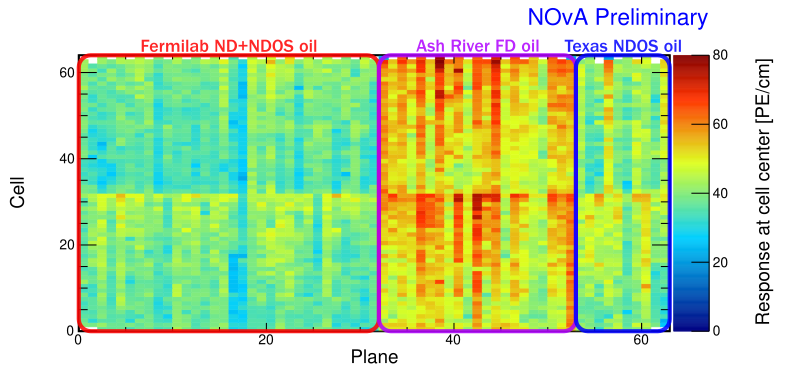
\includegraphics[width=\textwidth]{Plots/TestBeamScintillatorOils.png}
\caption{Uncorrected energy response in the centre of cells across the Test Beam detector showing a clear distinction between the different scintillator oils, shown with coloured boxes.}
\label{figScintillators}
\end{figure}

We can distinguish four samples of the NOvA scintillator oil used in the Test Beam detector:
\begin{itemize}
\item Mixed near detector production oil and NDOS-drained oil stored in a tanker and tanks outside in Fermilab \cite{NOVA-doc-38349};
\item Separate near detector production oil and NDOS-drained oil stored underground in barells at MiniBooNE \cite{NOVA-doc-33012};
\item Far detector production oil stored inside in Ash River in "totes" under several layers of black plastic \cite{NOVA-doc-34067};
\item NDOS-drained oil stored mainly inside at Texas A\&M University and University of Texas at Austin \cite{NOVA-doc-38740, NOVA-doc-39088}.
\end{itemize}

%The original plan \cite{NOVA-doc-34196} was to use the tanker and tank scinitillator for the entire Test Beam detector. However, due to extreme cloudeness of the scintillaotr in the tanks 

The original plan \cite{NOVA-doc-34196} was to only use the tanker/tank scintillator (sample 1). First tests showed acceptable results and the tanker oil was used to fill out almost the entirety of the first block of the detector (first 32 planes) \cite{NOVA-doc-38349}. However, when we loaded oil from tank two into the tanker, it became extremely cloudy and unusable, possibly due to contamination with water accumulated at the bottom of the tanks. The rest of the first block was therefore topped up with high quality scintillator from NDOS (sample 2). This is labelled as "Fermilab ND+NDOS oil" on Fig. \ref{figScintillators}.

%NDOS+ND scin3llator were stored in MEast tank farm in translucent tanks open to the atmosphere in 2016 [docdb:41229]
%docdb:41229 actually contains a pretty good description of the whole story

%First Tanker (2730 gallons pumped) used to fill 97.5% of first block ... Missing ~2.5 gallon top-off... Decided to use reserved NDOS 55-gallon drums... Used 65 gallons for detector, 11 gallons to clean up fill lines

%Even before the extreme cloudiness was discovered, it was known that the oil from the tanks has lost much of its original light yield properties. Reasons vary from water contamination to insects and dirt contamination \cite{NOVA-doc-34046-v2}. Yet it was still decided to use the tank 2 oil \cite{NOVA-doc-34196}. It was also decided not to mix the various oils (tanker/tank/NDOS/Ash River) as studying energy deposition in different types of oils could lead to some interesting insights \cite{NOVA-doc-34046-v2}.

%"One of the promising studies we see coming out of this is to understand the differences in performance for different type of energy depositions of scintillator A vs B vs C. " [docdb:34046]

The first 21 planes of the second block (planes 32 to 52) were filled with the far detector production scintillator shipped in from Ash River (sample 3) \cite{NOVA-doc-41961}. We again topped up these planes with the ND+NDOS scintillator (sample 2) \cite{NOVA-doc-41961}.

The last 10 planes (planes 53 to 62) \cite{NOVA-doc-41961} were filled with the "Texas" scintillator (sample 4), which has higher light yield than the one from the tanker, but lower than the Ash River one \cite{NOVA-doc-38740}.

%[docdb:38349] 2730 gallons of scintillator transferred to detector from the tanker. On April 16, circulated 20 gallons from tanker, and took scintillator sample. Extreme cloudiness meant 0\% light transmission (>=95\% required). Strongly suspect problem due to water accumulated at the bofom of tankers vented to the atmosphere since 2016, mixed with oil by pump. Used 2/4 reserved NDOS 55-gallon drums for top-off...  completed top-off of all Block 0 modules

In total the Test Beam detector is filled with 5418 gallons of scintillator oil with a weight of approximately 28.6 tons \cite{NOVA-doc-29543}.

\subsubsection*{Readout}
The Test Beam detector uses in total 126 Front End Boards (FEBs), each reading out signal from 32 cells (one module = half of a plane) \cite{NOVA-doc-29543}. The readout is located on the top and right side (when looking at the front) of the detector. 118 FEBs are version 4.1, same as in the Far Detector, and 8 FEBs, located in pairs on planes 16, 17, 48 and 49, are version 5.2, same as in the Near Detector. The Near Detector FEBs are designed to read out data in a fester rate and we used a mix of FEB types to study the difference in their response and to validate both versions in the same environment \cite{TeresaThesis}.

%The Near and Far Detectors use different front-end electronics since they handle different data volumes; the Test Beam Detector is instrumented with both types to facilitate a complete characterization of both NOvA neutrino detectors. [NOvATestBeam.pdf - Mike's proceedings]

\subsubsection*{Environment}
Unlike the near and the far detector, the Test Beam detector does not have any overburden to shield it from cosmic particles, which affects their rate and energies inside the detector. There is also less precise control of temperature and humidity than in the other detectors [source?], which can potentially impact the scintillator and readout performance.

%Is the HVAC the only systema that is controling the environment at MC7b?

%From docdb:29543
%Temperature very stable during winter months (heaCng is installed at MC7). However, dew point went over 10C ND shutdown threshold several times.
%Alex'es summary in docdb:30750:
%Ordered HVAC unit with electric reheat and dewpoint control, in essence over-cooling to maintain dewpoint then reheat to maintain temperature.

%Can I describe what is the shielding in MC7b? What is the white stuff from? It's basically the only thing shielding the detector from the cosmics and temperatures. Also need to say there is an HVAC system

%Placed in the Fermilab Test Beam Facility with no overburden. Describe environmental controls, temperature dependence etc. Maybe add plots from environmental control (temperature differences etc.) with descriptions of where were the readings taken.

\subsubsection*{Underfilled cells issue}
The Test Beam detector is slightly tilted around the Z axis by about 0.7$^{\circ}$ towards the readout. This caused the top cells of both modules of all the horizontal planes (cells 31 and 63) to be underfilled, creating an air bubble on the left side of the detector and severely affecting the energy response in those cells \cite{TeresaThesis}. This has been fixed \cite{NOVA-doc-49439} during the period 3 running by adding extensions to the filling ports and overfilling the horizontal cells with the ND+NDOS scintillator (sample 2).
%This scintillator was also used in the first half of the detector (Fermilab ND+NDOS oil on figure \ref{figScintillators}), but is different from the "Ash River oil" used in part of the second half of the detector (bright part of figure \ref{figScintillators}). The overfilling was done in April 2021 in 3 stages in between the full operation of the Test Beam detector.

%The detector is tilted around z axis towards the readout by about 0.7 degrees (the largest tilt is for the 11th plane of 0.79330 degrees. The ND has an oposite tilt of -0.2515 degrees on average (but also the readout is on the opposite side, so is it actually the same tilt?). Correcting this by 8 degrees would require lifting the east edge by at least 3.66cm, or to correct it to the ND tilt by lifting the east edge by 4.17cm. [docdb:47491 - this is the original talk by Teresa explaining the tilt on 21st Sep 2020]

%Also need to mention that the detector was then overfilled [docdb:49439 or 49827] but with a scintillator from the NDOS drums, causing the discrepancy between the high quality Ash River scintillator and the NDOS scintillator. But need to mention this after the scintillator part.
%The overfilling was done in three stages:
%\begin{enumerate}
%\item Overfilling the back 9 horizontal and the 7th horizontal from the front by April 21st
%\item Overfilling of the 15 front cells (except the 7th, which was already done, and the 14th, %with problems drilling vent hole) by April 27th
%\item Overfilling of the remaining 8 horizontals by April 30th
%\end{enumerate}

%From Teresa's thesis:
%The pitch and yaw of the detector was 2.464◦ around x and 0.487◦ around z. Roll (around beam direction) of each plane. Unfortunately, the direction of the roll means the east side of the detector is slightly lower than the west side. The east side is where the readout and fill ports for the scintillator are. As a result, the top cell in each horizontal module is underfilled, with an air bubble on the west side.

%%%%%%%%%%%%%%%%%%%%%%%%%%%%%%%%%%%%%%%%%%%%%%%%%%%%%%%%%%%%%%%%%%%%%%%%%%%%%%%
%%%%%%%%%%%%%%%%%%%%%%%%%%%%%%%%%%%%%%%%%%%%%%%%%%%%%%%%%%%%%%%%%%%%%%%%%%%%%%%
%%%
%%%                         Calibration description
%%%
%%%%%%%%%%%%%%%%%%%%%%%%%%%%%%%%%%%%%%%%%%%%%%%%%%%%%%%%%%%%%%%%%%%%%%%%%%%%%%%
\section{NOvA calibration process}
Test Beam is following the same ideas and procedures as the standard NOvA calibration. This section intends to provide only a brief overview of the NOvA calibration, with further details in the range of NOvA calibration technical notes \cite{NOVA-doc-13579}. All the code required for calibration is located in the \texttt{NOvASoft Calibration} package and the outline of the files and processes in NOvA calibration are shown on Fig. \ref{figCalibrationFlowchart}.

\begin{figure}[!hbtp]
\centering
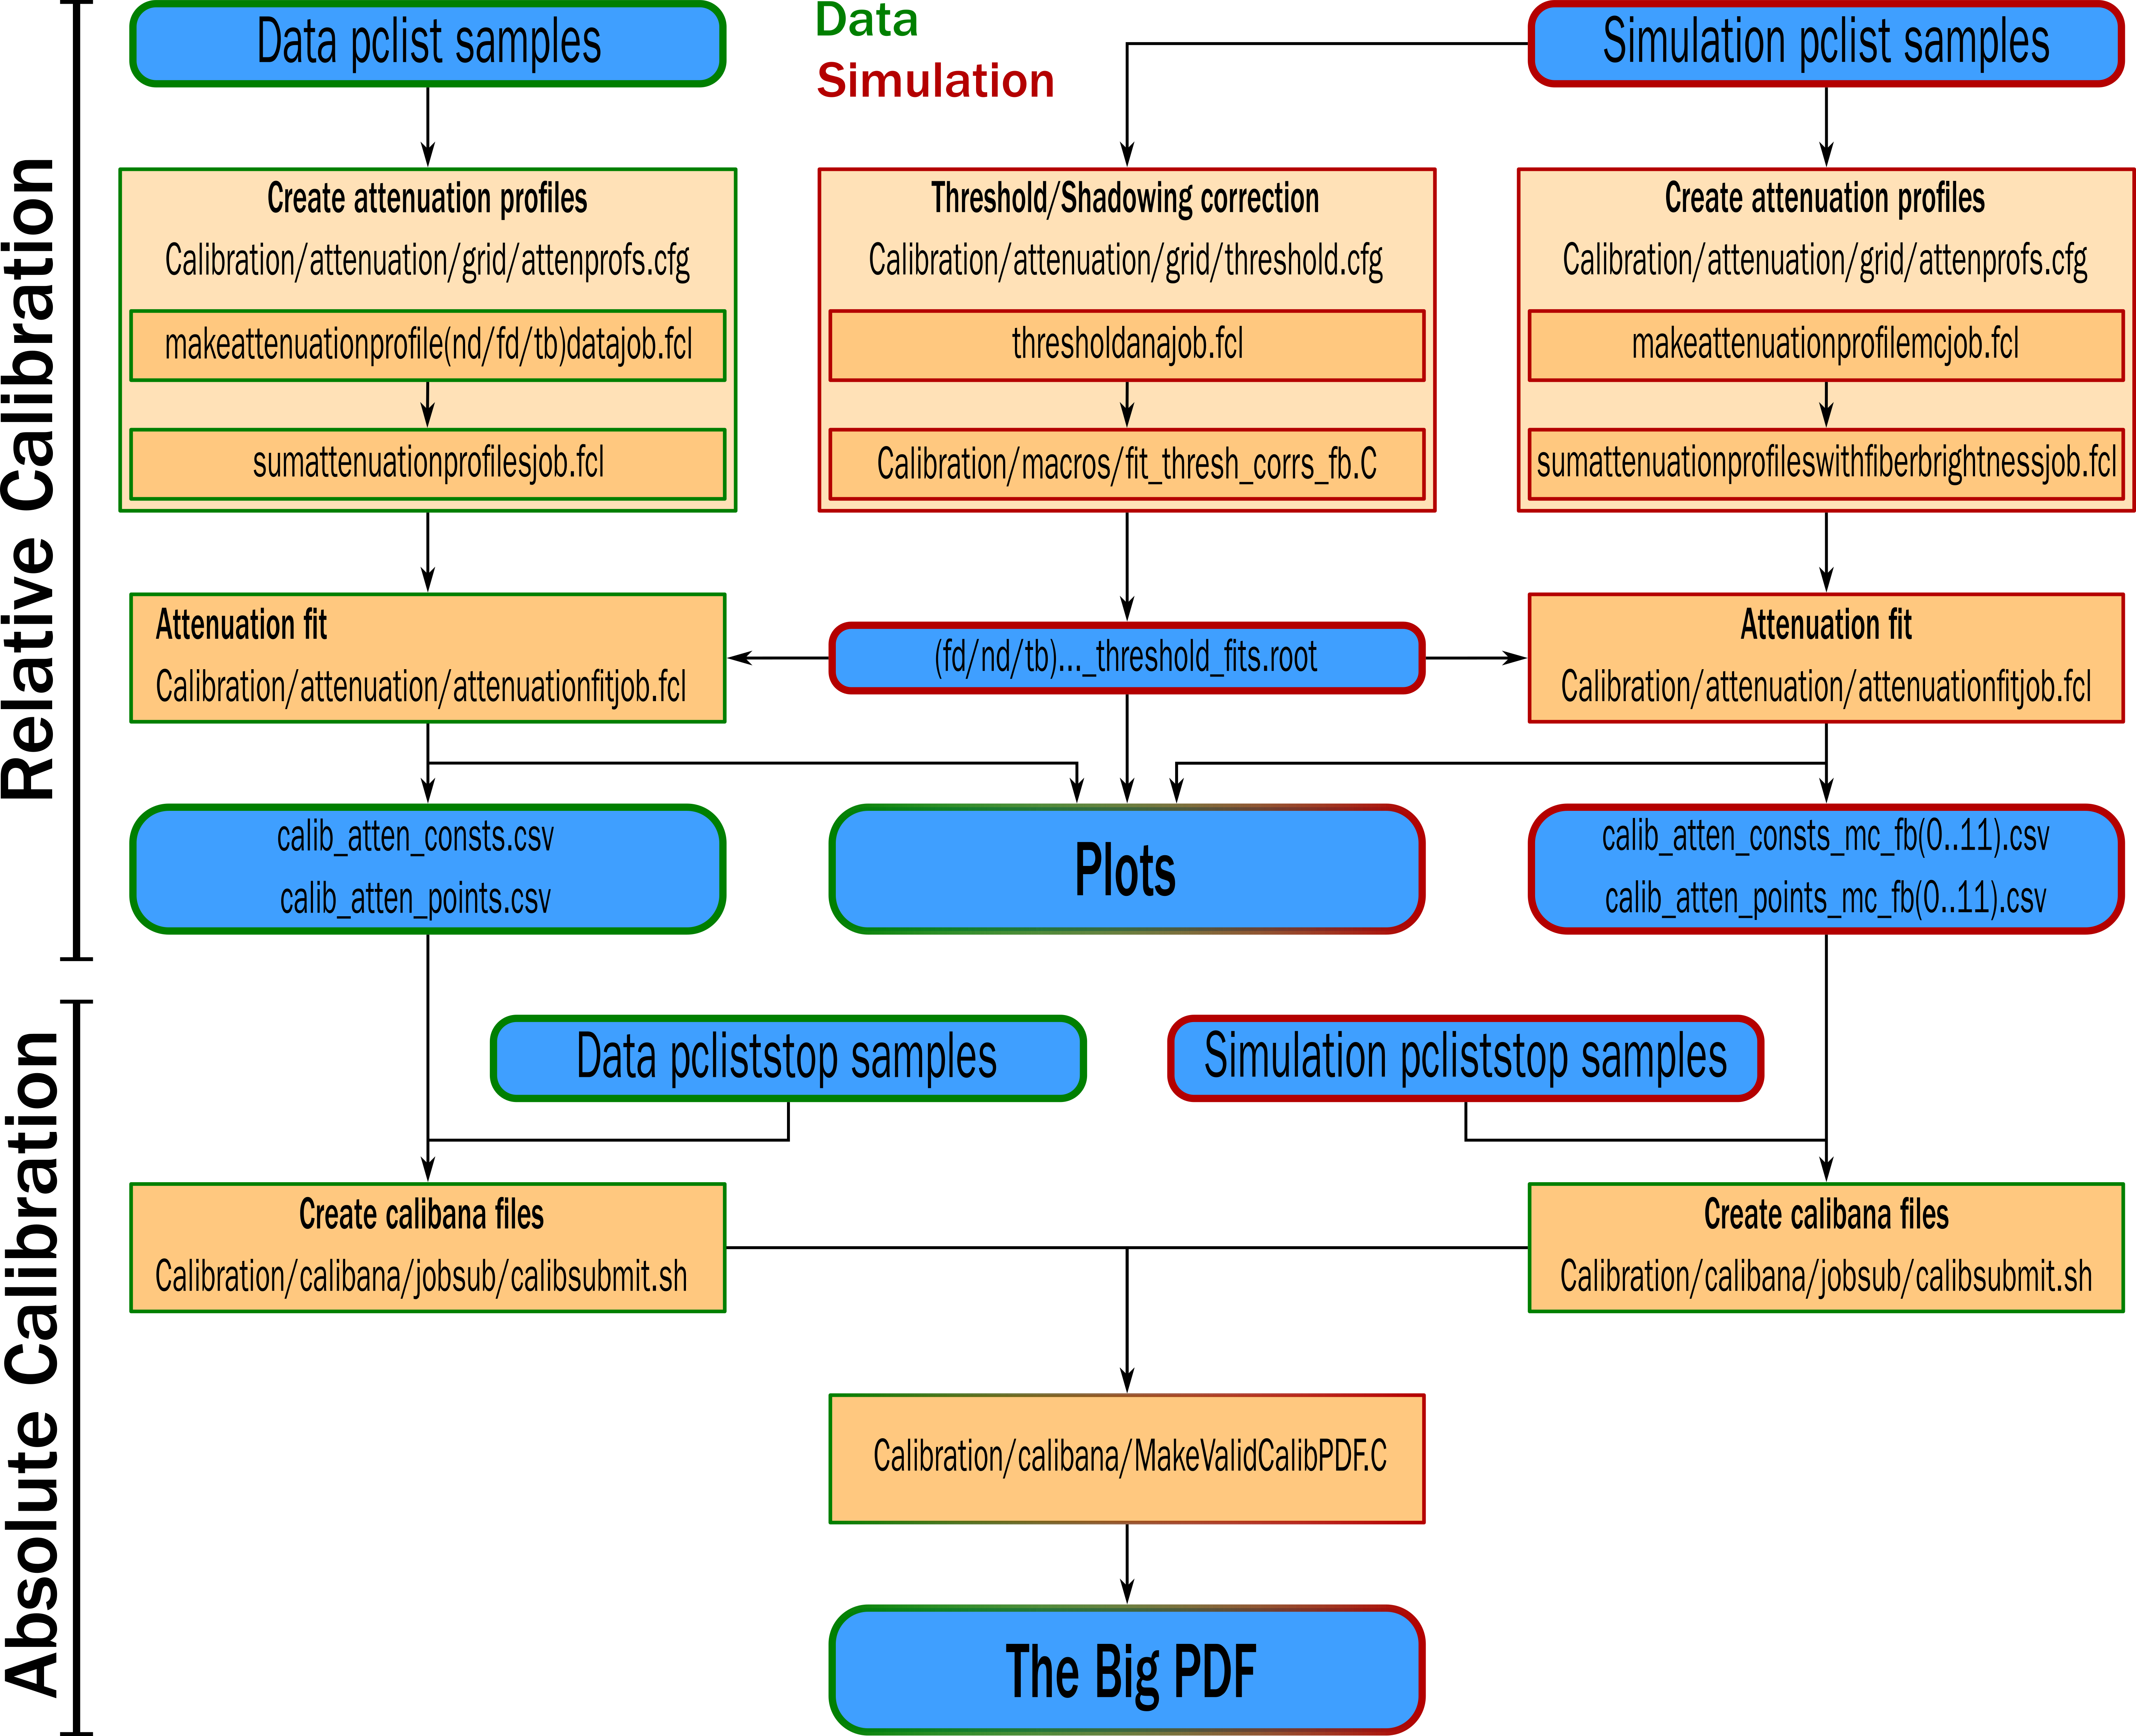
\includegraphics[width=\textwidth]{Plots/CalibrationFlowChart.png}
\caption{Flow chart showing the jobs (orange background) and files (blue background) needed and produced during the full NOvA calibration process. The left chain is showing the data calibration process (with green border) and is applied to every data calibration sample separately (periods or epochs). The center and right chains are showing the simulation calibration process (red border), which is redone only if there's a change to the detector simulation. The absolute calibration at the bottom combines data and simulation. The entire process is done separately for each NOvA detector.} 
\label{figCalibrationFlowchart}
\end{figure}

The purpose of calibration is to make sure that we get the same amount of energy wherever or whenever it's deposited in whichever of NOvA's detectors and to express this amount of energy in physical units. The NOvA calibration uses cosmic ray muons, which provide a consistent, abundant, and well-understood source of energy deposition and consists of two parts \cite{NOVA-doc-7410}:
\begin{enumerate}
\item The \textbf{relative calibration} corrects for attenuation of scintillator light as it travels through the cell to the readout, as well as for differences between detector cells. This correction is calculated for each cell separately.
\item Followed by the \textbf{absolute calibration}, which only uses stopping muons when they are minimum ionising particles. In the absolute calibration we calculate a scale between the measured energy deposition, corrected by the relative calibration, and the simulated energy deposition in physical units of $\unit{MeV}$. This scale is calculated for each time period and each detector separately, which ensures the energy deposition is directly comparable wherever or whenever it occurred.
\end{enumerate}

The NOvA calibration process technically also involves \textbf{timing calibration}, which corrects for the time differences of the signal to be processed \cite{NinerThesis}. However, this is done as a separate project to the relative and absolute calibrations and is out of scope of this technical note.

%Should I talk about drift now already?

%Calibration is necessary to convert electronic signals to physically meaningful energy in units of GeV. Two calibration steps precede the calorimetric energy calibration. First raw ADCs (Analogue Digital Conversion) are converted to units of photo-electrons (PE) using the known average response of the APDs; secondly an attenuation calibration corrects for the position dependent response [6]. A drift calibration may be included in the future to correct for changes in detector response over time. The calorimetric energy scale calibration is the last step in the calibration chain and the detector response should already be uniform in space and eventually also in time. [docdb:13579 - FA\_Calorimetric\_energy\_scale]

%Using the average expected APD response, integrated charge from the ADCs are converted to units of photo-electrons (PE) [SA Absolute energy scale]

%I think I should actually include some kind of a description of the ADC to PE conversion.
\iffalse
The scaling of the ADC to PE depends only on the gain and the version of the FEB. Otherwise it's just a very simple scaling (explain this at the PE definition):
\begin{equation}
PE=\frac{\textsf{peakADC}}{\textsf{ADCPerPE}},
\end{equation}
\begin{equation}
\textsf{ADCPerPE}=\textsf{Gain}\times\frac{4095}{ADCScale}
\end{equation}
where ADCScale is 217000 for FEBv4.1 and 204800 for FEBv5.2.
\fi

%The PECorr scaling is 75.0 (NDOS), 37.51 (ND), 39.91 (FD) and 39.91 (TB)

The basic units and variables used to define energy deposited in the NOvA detectors are listed in table \ref{tabCalibrationVars}.
\begin{table}[!ht]
\centering
\def\arraystretch{1.4}
\begin{tabular}{m{0.1\textwidth} m{0.86\textwidth}}
ADC & The digitized charge collected by the APDs from the \textbf{A}nalog to \textbf{D}igital \textbf{C}onverter \cite{NOVA-doc-13518}.\\
PE & Number of \textbf{P}hoto \textbf{E}lectrons. Calculated by a simple rescaling of the best estimate of the peak ADC. The PE per ADC scale only depends on the FEB type and the APD gain settings. This conversion is done before the calibration and PE serves as the base unit for calibration.\\
PECorr & \textbf{Corr}ected \textbf{PE} after applying the relative calibration results. The correction is a ratio between an average energy response (a pre-determined semi-arbitrary number) and the result of the the relative calibration fit (also called attenuation fit), which depends on w, cell, plane, epoch and detector. This makes the energy response equivalent across each detector.\\
MEU & \textbf{M}uon \textbf{E}nergy \textbf{U}nit is the mean detector response to a stopping cosmic minimum ionising muon.  For true variables it's equivalent to the mean MeV/cm and for reconstructed variables to the mean PECorr/cm.\\
MeV & Estimated energy deposited in the scintillator calculated from PECorr using the results of the absolute calibration. Additional correction for dead material needs to be made in order to get an estimate of the calorimetric energy.
\end{tabular}
\caption{Definitions of variables commonly used in calibration \cite{NOVA-doc-13579,NOVA-doc-7410}.}
\label{tabCalibrationVars}
\end{table}

The final result of the NOvA calibration is the deposited energy in terms of physical units, which is in effect calculated as:
\begin{equation}
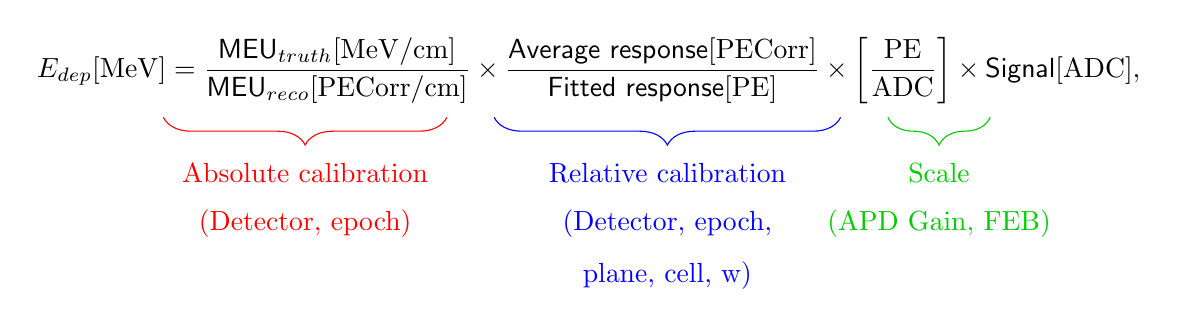
\begin{tikzpicture}[baseline=(current  bounding  box.center)]
\node {\(\displaystyle
E_{dep} [\unit{MeV}]=\frac{\textsf{MEU}_{truth} [\unit{MeV/cm}]}{\textsf{MEU}_{reco} [\unit{PECorr/cm}]}\times \frac{\textsf{Average response} [\unit{PECorr}]}{\textsf{Fitted response} [\unit{PE}]}\times \left[\frac{\unit{PE}}{\unit{ADC}}\right] \times \textsf{Signal} [\unit{ADC}],
\)};
\draw[decorate,decoration={brace,amplitude=10pt,mirror},red] (-5.4,-0.6) -- (-1.8,-0.6) node (A) [midway,yshift=-20pt]{Absolute calibration};
\node[below,yshift=-10pt,red] at (A) {(Detector, epoch)};
\draw[decorate,decoration={brace,amplitude=10pt,mirror},blue] (-1.2,-0.6) -- (3.2,-0.6) node (B) [midway,yshift=-20pt]{Relative calibration};
\node[below,yshift=-10pt,blue] (B2) at (B) {(Detector, epoch,};
\node[below,yshift=-10pt,blue] at (B2) {plane, cell, w)};
\draw[decorate,decoration={brace,amplitude=10pt,mirror},green!80!black] (3.8,-0.6) -- (5.1,-0.6) node (C) [midway,yshift=-20pt]{Scale};
\node[below,yshift=-10pt,green!80!black] at (C) {(APD Gain, FEB)};
\end{tikzpicture}
\end{equation}
where both the relative calibration results (blue fraction) and the absolute calibration results (red fraction) are stored in a database and applied together with the ADC-to-PE scale by the \texttt{NOvASoft Calibrator} package during processing of every hit in the NOvA detectors.

%The light is attenuated while traveling through the fiber. To find the correct energy of the incident particle these losses are corrected by using cosmic ray muons. The cosmic ray muons are used to calibrate the NOvA detectors because they provide a source of consistent energy across the detectors. The purpose of the attenuation calibration is to provide constants and formulae such that an amount of energy deposited in the detector and registered by an APD can be expressed in comparable units, PECorr which are the corrected photo-electrons (PE) no matter where the deposition occurred. Variations in time are to be handled by the drift calibration. The purpose of the absolute calibration is to provide a scaling factor, independent of channel since all of that variation should have been taken out by the relative calibration, so that energy deposits can be expressed in physically meaningful units (GeV).
%For both purposes cosmic rays are used as probes. For the attenuation calibration they represent a source of consistent energy deposits across the detector of approximately 1 minimum ionizing particle’s energy, MIP, but this is not assumed. Any average value consistent across the detector would do. For absolute calibration, stopping muons are used, whose precise energy deposits should be estimateable from the Bethe Bloch formula. [docdb:13579 - SA The Attenuation and Threshold Calibration of the NOvA detector, but a lot of this is actually just copied from Backhouse's original calibration technote docdb:7410]

%(Dividing data into periods and epochs) A new period is started for a major change to running conditions such as a horn current change, a long shutdown, target replacement, etc. Periods are divided into epochs. A new epoch is started whenever analysis or production reasons dictate. Calibration has been performed for all the periods separately and has used the data that are determined by the Data Quality group to be good. The effects of aging, temperature, partial filling, and cooling are neglected. The drift calibration should be able to account for all of these (but drift calibration doesn't really exist yet afaik). [docdb:13579 - SA The Attenuation and Threshold Calibration of the NOvA detector]

\subsubsection*{Creating calibration samples}\label{secCreatingCalibrationSamples}

We want to select good quality cosmic ray muons. First, we remove beam related events based on their time stamps relative to the time of the beam spill, using the \texttt{RemoveBeamSpills} (for the near and far detectors), or \texttt{RemoveTBSpills} filter (for the Test Beam detector), as shown on Fig. \ref{figRemoveBeamSpill}. Next we apply reconstruction to get the CellHit, slicer, and track information, followed by a track-based selection to remove misreconstructed and poor quality events.

\begin{figure}[hbtp]
\centering
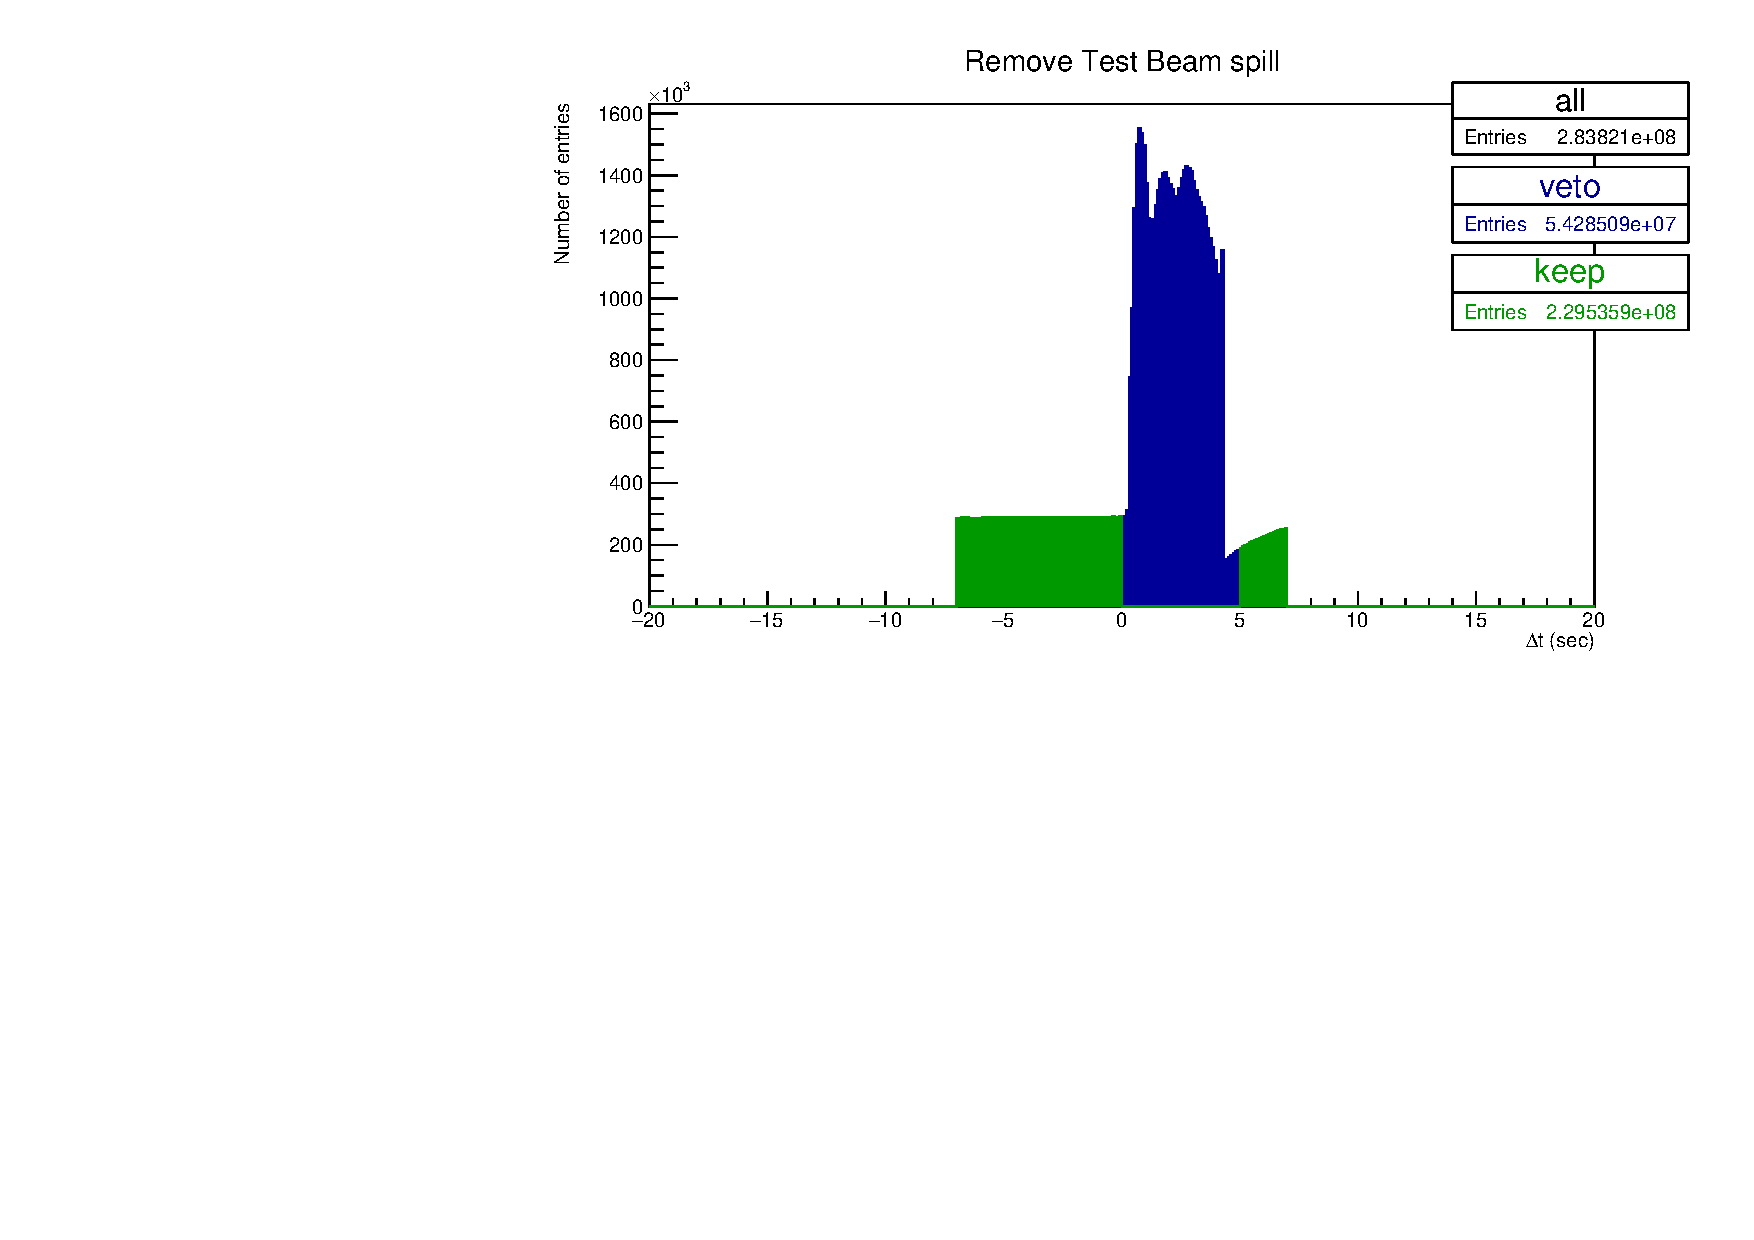
\includegraphics[width=\textwidth]{Plots/RemoveTBSpills.pdf}
\caption{Test Beam beam spill events removed from the calibration samples. Test Beam beam spill is 4.2 seconds long and we remove events (in blue) within a 5 seconds window from the start of the beam spill. The remaining events (green) should mostly consist of cosmic particles. This example and the numbers of entries are for the full period 4 Test Beam sample.}
\label{figRemoveBeamSpill}
\end{figure}

Since energy deposition depends on the path length particle travels through a cell, we only use hits for which we can reliably calculate their path length. We call these hits \textbf{tricell} hits, as we require that all accepted hits are accompanied by a recorded hit in both neighbouring cells of the same plane, as shown on Fig. \ref{figTricellCondition}. In case there is a bad channel in a neighbouring cell, we ignore this channel and look one cell further. We can then calculate the path length simply as the cell width divided by the cosine of the direction angle \cite{NOVA-doc-13579,NOVA-doc-7410}.

\begin{figure}[hbtp]
\centering
\begin{subfigure}[b]{0.49\textwidth}
\centering
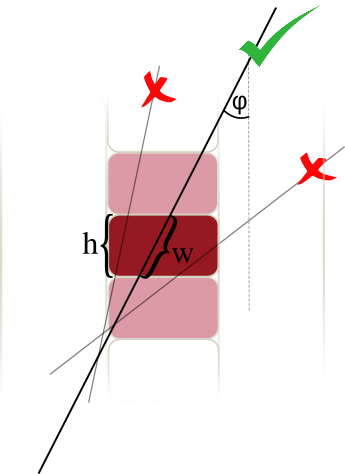
\includegraphics[width=0.6\textwidth]{Plots/TricellConditionWithDescription.png}
\caption{}
\end{subfigure}
\begin{subfigure}[b]{0.49\textwidth}
\centering
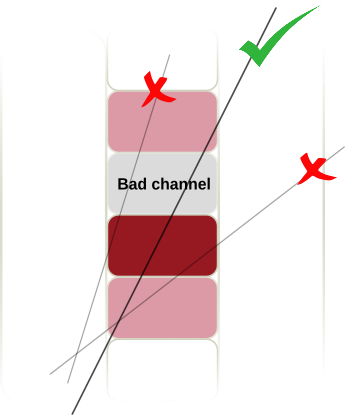
\includegraphics[width=0.6\textwidth]{Plots/TricellConditionWithBadChannel.png}
\caption{}
\end{subfigure}
\caption{Illustration of the tricell condition (a). We only use hits that have two surrounding hits in the same plane to be used in the NOvA calibration. This is to ensure a good quality of the path length (d) reconstruction, which is calculated from the known cell height (h) and the reconstructed track angle $\left(\varphi\right)$. In case the hit is next to a bad channel (b), we ignore this bad channel and require a hit in the next cell over.}
\label{figTricellCondition}
\end{figure}

%Do I even need to talk about the Z estimate, Avg estimate, or the 

%The first step in the attenuation calibration is to select the suitable hits from tracks of cosmic ray muons. Because a reliable estimate of pathlength is required, not all hits are suitable for use.  If a cell has each of its neighbors in the same plane hit, then we know, for a Y view cell, that the track entered through the upper wall, and exited through the lower wall. The pathlength then is just the width of the cell divided by the direction cosine. This selection also significantly decreases the chance that the hit in question is a noise hit. Allowance is made for neighboring dead cells, so e.g. “hit, dead, hit, hit” would still lead the 3rd cell to be selected. The second best hit selection, in cases where there are too many dead neighboring cells on each side, is the so-called “z” estimator, where a hit is required at the same cell number in each of the neighboring planes in the same view. The pathlength is then the ratio of cell depth to cz.[docdb:13579 - SA The Attenuation and Threshold Calibration of the NOvA detector, copied from docdb:7410]

%from docdb:7410: A requirement that the track be “throughgoing” (lowest endpoint outside the fiducial volume) was applied, but doesn’t make much difference. I think this selection was broken by the recent changes to StopperSelection anyway. (So it seems that it was required for the relative calibration that the muons are through-going, but I assume this was discarded somewhere down the line)

For the absolute calibration we select muons that stop inside the detector, by identifying muons with a Michel electron at the end of their track \cite{NOVA-doc-13579-FACalorimetricEnergyScale}.

%Stopping muon selection (from docdb:13579 - FA\_Calorimetric\_energy\_scale): There are two avenues for selecting stopping muons; i) selecting tracks whose reconstructed end point is contained within the detector and ii) selecting tracks that have a Michel electron at one end. Michel electrons are useful for both identifying muons and effective tagging of the end point of muon tracks. The stopping selection requires the reconstructed end point of the muon track to be at least 50 cm from the detector edge. The identification of a Michel electron at the end of a muon track has two stages of both temporal and spatial range requirements. Firstly, a candidate Michel electron hit is required to occur between 1 and 30 microseconds after the mean time of the hits on the track. Furthermore, the candidate Michel electron must be within a 30 cm sphere surrounding the reconstructed track end point. The candidate Michel electron hit for a muon track is the hit that produces the largest detector response among the hits that pass the above cuts. Secondly, cell hits surrounding the candidate Michel electron hit are associated with the Michel electron if they occur within a 30 cm sphere surrounding the Michel electron candidate. Furthermore, to be associated with the Michel electron the cell hits must occur between 0.5 microseconds before and 0.5 microseconds after the candidate Michel electron. Michel electrons at the end of muon tracks are reconstructed using the candidate and associated Michel electron hits. The stopping muon selection requires a Michel electron at the end of the muon track.

For each data period or epoch and for each version of the simulation we create two calibration samples that are used as the input for the relative and absolute calibration. The samples are called \cite{NOVA-doc-13579-CalibrationMetaREADFIRST}
\begin{itemize}
\item pclist = \textbf{list} of \textbf{p}re-\textbf{c}alibrated hist; Contains all selected cosmic muon events and is used in the relative calibration;
\item pcliststop = pclist files only containing stopping muons used for the absolute calibration 
\end{itemize}

\subsubsection*{Fibre brightness}

For data, the relative calibration is done for each individual cell in each plane to properly account for any potential variations, repeating the attenuation fit $N_{cell}\times N_{plane}$ times. However, generating enough simulated events turned out to be computationally expensive. Therefore, assuming the simulated detector is approximately uniform plane to plane, for simulation we can "consolidate" the detector planes and only consider variations in the two views. Therefore for simulation we would repeat the fit $N_{cell}\times N_{view}$ times \cite{NOVA-doc-13579-SAAttenuationAndThreshold,NOVA-doc-34909}.

However, there are some variations in the detector response cell by cell that can be caused by different fibre brightnesses, but also by different qualities of the scintillator, air bubbles, APD gains, looped or zipped fibres and potentially others. We want to include these variations in the simulation to better match data. To emulate these differences in the simulation without the need to simulate every cell individually, we divide each detector into 12 brightness bins, as shown on Fig. \ref{figFiberBrightnessBins}. These brightness bins describe the relative differences in the detector response between individual cells \cite{NOVA-doc-34909}. Therefore in the end, for simulation we perform the attenuation fit $N_{cell}\times N_{view}\times N_{BrightnessBin}$ times.

%Do I need to describe here how we do it or is it enough if I just say that we do?
%To divide the detector into brightness bins, we use the results of the attenuation fit and look at the fitted response at cell centre, which should represent the average response in that cell. Then we normalize the 

\begin{figure}[hbtp]
\centering
\begin{subfigure}[b]{0.495\textwidth}
\centering
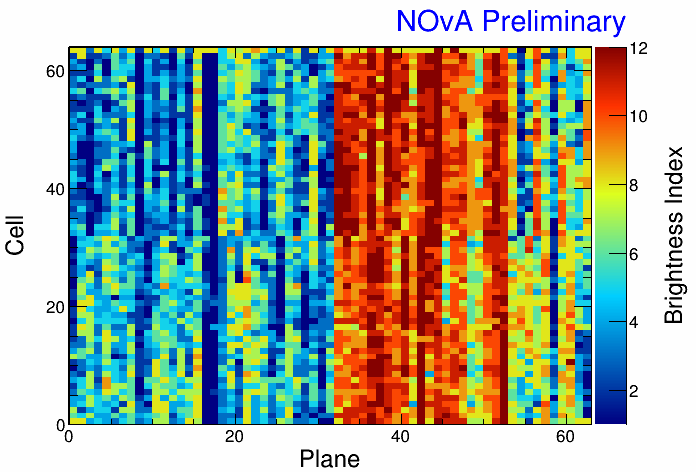
\includegraphics[width=\textwidth]{Plots/BrightnessIndex.png}
\end{subfigure}
%\hfill
\begin{subfigure}[b]{0.495\textwidth}
\centering
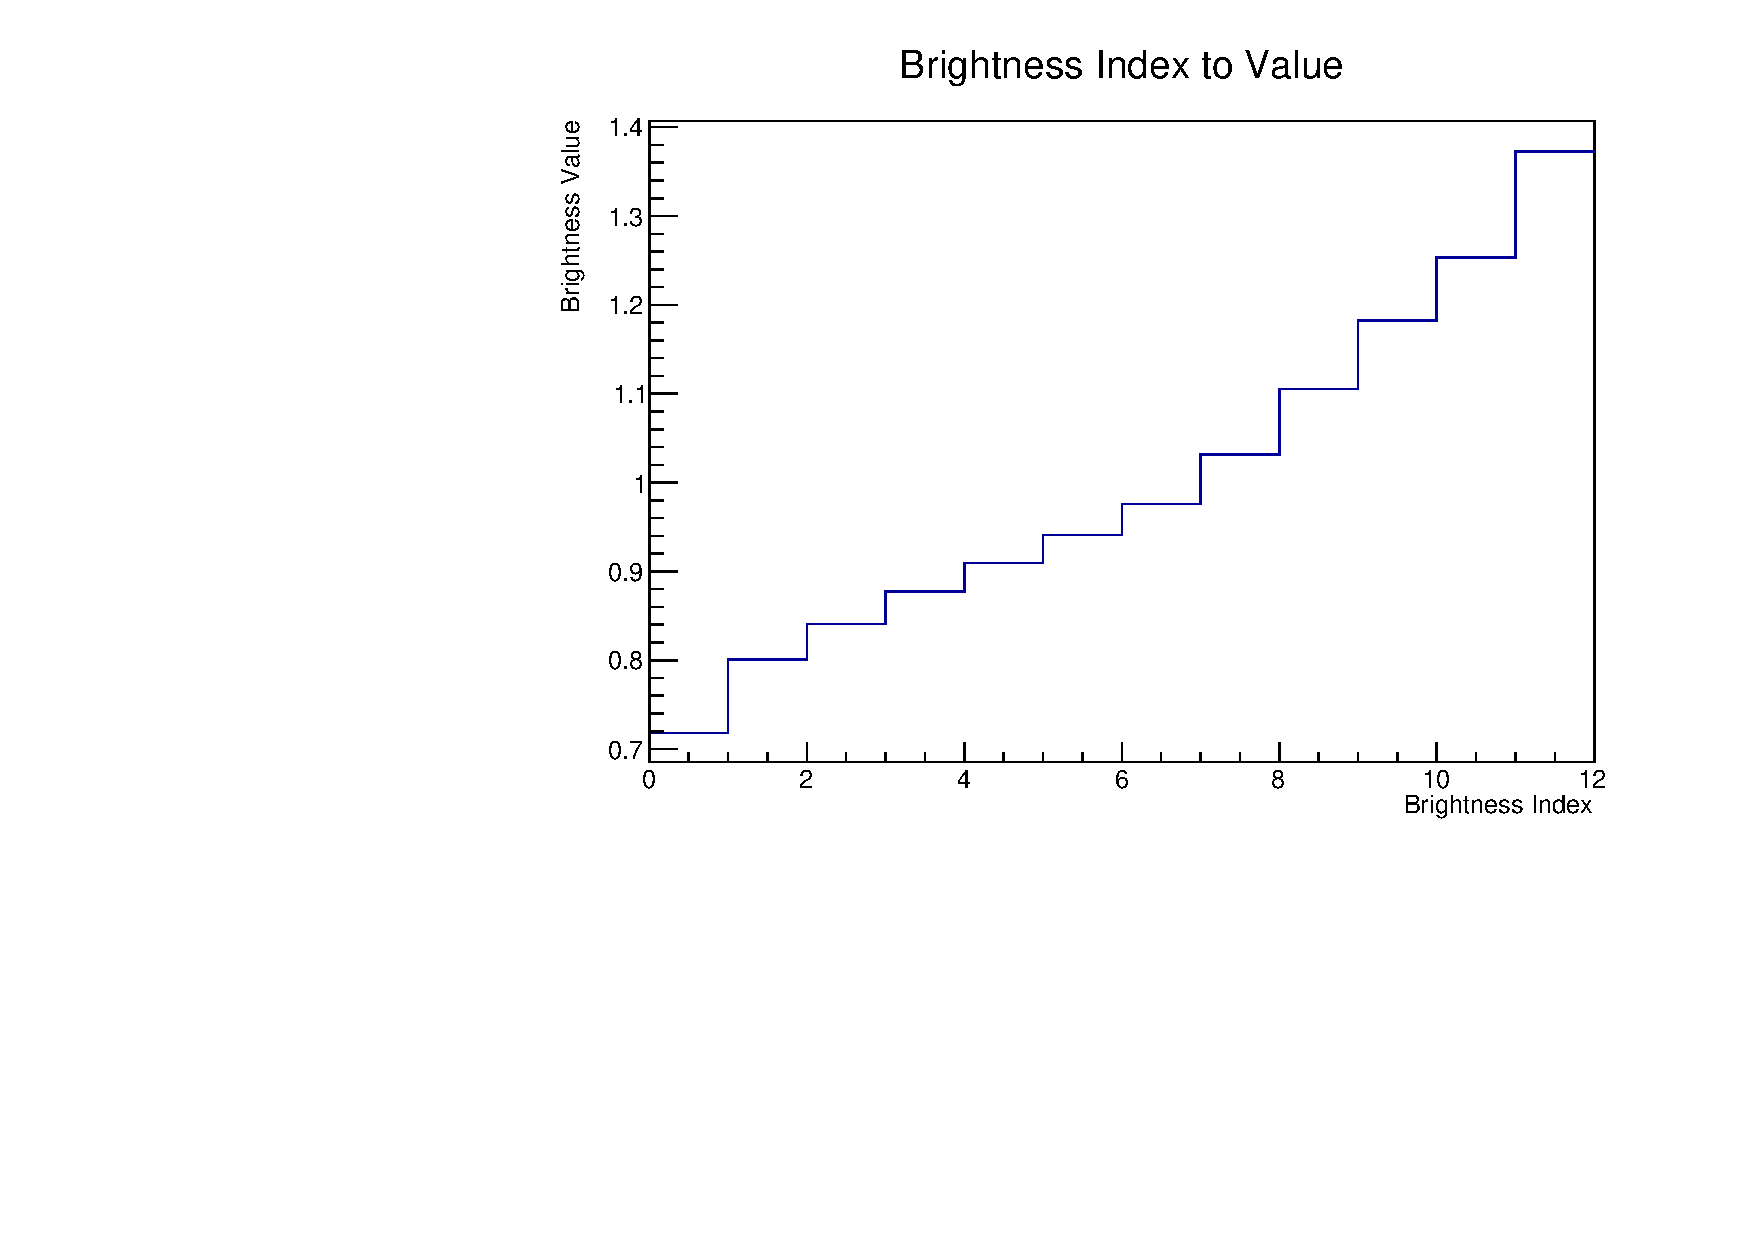
\includegraphics[width=\textwidth]{Plots/BrightnessIndexToValue.pdf}
\end{subfigure}
\caption{The Test Beam detector is (like the standard NOvA detectors) divided into 12 brightness bins (left plot), each representing a relative difference in energy response (right plot) due to different brightnesses of the fibres, scintillators, or readout.}
\label{figFiberBrightnessBins}
\end{figure}

To divide each detector into the 12 brightness bins, we use results from the relative calibration. Specifically we take the result of the attenuation fit (equal to the average response) in the centre of each cell to fill a 2D histogram. Then we normalize this histogram by dividing the response in each $\textsf{Cell}\times\textsf{View}\times\textsf{Plane}$ by the average response in the corresponding $\textsf{Cell}\times\textsf{View}$. All uncalibrated cells get assigned the average response (1 in normalized histogram). Then we make a 1D histogram filled with the normalized responses of each cell and divide this histogram into 12 equally populated bins (so each bin represents approximately the same number of detector cells, shown on the left plot of Fig. \ref{figFiberBrightnessBins}). The mean normalized response in each bin represents the relative brightness value of this bin (right plot of Fig. \ref{figFiberBrightnessBins}). A ROOT file with the distribution of brightness bins across the detector and their corresponding relative brightness values is stored inside the \texttt{NOvASoft PhotonTransport} package as \texttt{<det>BrightnessFromCosmics.root}.

\subsubsection*{Threshold and shielding correction}

Energy deposited far away from the readout may get attenuated enough to be shifted below the threshold. These low energy depositions would be missing from the attenuation fit, biasing it towards larger light levels with increasing distance from the readout. Similar effect, specifically for the vertical cells, is caused by using cosmic muons for calibration and applying it to beam muons. The top of the detector effectively shields the bottom, skewing the energy distribution of cosmic muons. To correct for both of these effect, we use the simulation pclist sample to calculate the threshold and shielding (also called threshold and shadowing) correction by comparing the true and reconstructed information. We apply this correction before the attenuation fits \cite{NOVA-doc-13579-SAAttenuationAndThreshold}.

%Should I write anything more? Maybe about how do we calculate this more specifically, or that it's done for view X fb bin X cell X w

%In the Far Detector data and MC a large divergence between calibrated and true energies as a function of W was observed [8]. This was traced back to the much longer cell lengths in the FD meaning that thresholds play a large role at the foot of a cell. Also self-shielding of the detector by its own mass lay a role in the observed discrepancy. Thresholds mean that for a hit to be seen by an APD, it may need to have a slight upwards fluctuation in the number of photons produced by the energy deposition. Self-shielding means that the average visible energy depositions from MIPs are not truly spatially uniform in the detector. If not corrected for these effects, there will be a bias in the set of hits that the attenuation fit sees, and leads it to overestimate the light-level, and so under-estimate real hit energies by tens of percent. The approach adopted to solve this problem was to create a correction factor as a function of view, cell, and position along the cell which would be applied before the attenuation correction to remove the effect of thresholds and shielding. To this end MC truth information about the calibration hit sample is used to create a combined threshold and shadowing correction for each cell and view combination,
%\begin{equation}
%T=\frac{PE}{\lambda}\frac{E_{true}}{E_{mip}},
%\end{equation}
%where $T$ is the combined “threshold and shielding” correction factor, $PE$ is the simulated photoelectrons recorded at the readout, $\lambda$ is the number of simulated photons which would be seen at the readout out in the absence of fluctuations, $E_{true}$ is the true energy deposited in the cell and $E_{mip}$ is the naive energy you would expect to be deposited based on the pathlength through the cell. In this way it encodes a threshold correction based on the simulated readout PE with and without the fluctuations, with $\lambda$ dependent on your simulated threshold, as well as a shielding correction based on the simulated energy deposition and a naive no shielding approximation. This equation gives us a cell by cell correction but we use an empirical polynomial fit to that distribution which removes statistical noise from the correction and well describes the initial distribution. This correction factor is applied to the cell by cell data and MC PE/cm distributions before the attenuation fits. [docdb:13579 - SA The Attenuation and Threshold Calibration of the NOvA detector, reference 8 is for docdb:7247, a talk by Backhouse]

\subsection{Relative calibration}\label{secRelativCalibration}

%Detailed description can be found in the "Instructions for the Attenuation Calibration Job" technote from Prabhjot from docdb:13579 (list of all calibration technotes) and on the relative calibration wiki page.

Relative calibration corrects for the attenuation of the scintillator light by fitting the average detector response over the position in each cell (w), separately for every cell inside each detector. Dividing the "average response" of the detector by the result of the attenuation fit for each $\textsf{Plane}\times\textsf{Cell}\times\textsf{w}$ combination effectively removes relative differences within and between all cells across the entire detector. The average response is a single constant number chosen to approximately represent the average response in the middle of the cell. Its value is for the far detector and Test Beam 39.91~PE/cm and for the near detector 37.51~PE/cm. The value of the average response has no impact of the calibration results, as the absolute scale of the detector response is determined during the absolute calibration and relative calibration only serves to remove the relative differences \cite{NOVA-doc-7410,NOVA-doc-13579-SAAttenuationAndThreshold}.
 
To create the attenuation fit we use the following procedure \cite{NOVA-doc-7410}:
\begin{enumerate}
\item Create the \textit{attenuation profiles}. Attenuation profiles are essentially profile histograms of detector response in terms of $\unit{PE/cm}$ as a function of position in the cell (w) for each cell in all planes. We construct the attenuation profiles over a little wider range than the actual length of the cell and always with 100 bins for each detector. This means that smaller detectors, like the Test Beam detector, have a finer binning ($\sim 3\unit{cm}$/bin) compared to the Far Detector ($\sim 18\unit{cm}$/bin).
\item Analyse the attenuation profiles. The job to create the attenuation profiles also creates validation histograms, which should be analysed prior to performing the attenuation fit to make sure the attenuation profiles look as expected.
\item Apply the threshold and shielding correction that was created before the relative calibration.
\item Do the attenuation fit over the full length of each cell. The fit consists of
\begin{enumerate}
\item an exponential fit, which combines two cases. First, when the scintillating light travels the short distance straight to the readout, and second, when it goes to the far side of the cell and loops around before going to the readout. The fitted function has a form:\\
\begin{equation}
y=C+A\left(\exp\left(\frac{w}{X}\right)+\exp\left(-\frac{L+w}{X}\right)\right),
\end{equation}
where $y$ is the fitted response, $L$ is the length of the cell and $C$, $A$ and $X$ are the fitted parameters. $X$ also represents the attenuation length.
\item Smoothing of the residuals from the exponential fit, mainly at the end of cells, with the LOcally WEighted Scatter plot Smoothing (LOWESS) method.
\end{enumerate}
\item Check the plots of the attenuation fit for a selection of cells.
\item Save the fit result to the database in the form of two csv tables. The \texttt{calib\_atten\_consts.csv} table holds the results of the exponential fit, together with the final $\chi^2$ of the fit. The \texttt{calib\_atten\_points.csv} table holds the results of the LOWESS smoothing.
\end{enumerate}

To ensure the quality of the attenuation fit, we only apply the results if the final $\chi^2<0.2$. If $\chi^2>0.2$, we ignore the results for this cell and mark it as \textit{uncalibrated}.

%Attenutation profiles have a constant binnin fNBins=100 (in w), same for ND, FD and TB. This results in an effectively finer binning for TB compared to ND and FD. For FD w = (-900,+900), ND: (-250,+250), TB: (-150,+150). TB: 3cm/bin, ND: 5cm/bin, FD: 18cm/bin. What effect could this have on the relative calibration results? Particularly on the calibration shape?

%where y is the response, L is the cell length, C, A and X are the free parameters in the fit. X gives the attenuation length as well. Initially, the fit is to the central part of the cell, which is different for each detector. In addition to the approximately quartic behavior at the ends of every channel there are in many channels fairly large residuals. They don’t appear to follow any consistent pattern. The leading hypothesis is that these are due to varying fiber position within the cell. Usually the fiber lies in the corners of the cell, but if it is somehow twisted so that it rises into the center of the cell, then it should collect more light, to an extent comparable to what is seen here. To remove such an irregular pattern, the residual from the analytic fit is simply fit with LOcally WEighted Scatter plot Smoothing, LOWESS. The LOWESS curve at each point is formed from the weighted mean of the deviations. The weighting function is the traditional tri-cube, (insert equation, likely not needed for this technote) [docdb:13579 - SA The Attenuation and Threshold Calibration of the NOvA detector, already in 1stAna and Backhouse's technote]

%For NDOS the fit was a very little bit different, where we didn't use $L$ but $3L/2$. Also it says that "Over the length of an NDOS cell, the effect of the long attenuation length is imperceptible, and is modelled as a constant (If you put a long attenuation term in, the fit drives the length scale to infinity anyway). [docdb:7410]

%In many channels, fairly large residuals are visible. They don’t appear to follow any consistent pattern. The hypothesis is that these are due to varying fibre position within the cell. Usually the fibre lies in the corners of the cell, but if it is somehow twisted so that it rises into the centre of the cell, then it should collect more light, to an extent comparable to what is seen here. To remove such an irregular pattern, the residual from the analytic fit is simply fit with LOWESS (locally weighted scatterplot smoothing). The LOWESS curve at each point is formed from the weighted mean of the deviations. The weighting function is the traditional tri-cube:
%\begin{equation}
%w_i=\left(1-\left|\frac{x-x_i}{\sigma}\right|^3\right)^3.
%\end{equation}
%The smoothing length scale $\sigma$ is 30cm. 20 points calculated by this method are stored, to be linearly interpolated between to approximate the full LOWESS curve. If the LOWESS fit at any point exceeds 15\% the original attenuation fit was very bad, and the channel is marked uncalibrated. Figure 4 shows an example of large (10\%) deviations being fitted. This variation is not seen in the MC, and so the LOWESS fit is skipped there. Due to the lower stats available in MC, instead of being collated by plane and cell, the curves are only calculated by view and cell. [docdb:7410]

%The current value of $\sigma$ in the code is $1.5\times\textsf{DetWidth}/20$

\subsection{Absolute calibration}

To find the absolute energy scale, we apply the relative calibration results on the stopping muon sample and look at the energy they deposited in cells 1-2 meters from the end of their tracks. In this track window they are approximately minimum ionising particles and their energy deposition is almost constant and well understood. Additionally, we don't use hits from the edges of a cell, as those might be affected by the lower number of events, fibre endings, or loops. 

For each calibrated data and simulation sample we take a mean of the corrected deposited energy distribution, separate for each view. We then take a simple average from the two views to get the final $\textsf{MEU}_{reco}$ in units of $\unit{PECorr/cm}$ for each sample \cite{NOVA-doc-13579-FACalorimetricEnergyScale}. Additionally, from simulation we can get the mean of the distribution of the true deposited energy in the scintillator, $\textsf{MEU}_{truth}$ in units of $\unit{MeV/cm}$ for the same sample of stopping muons. 

We ignore the energy that is lost in the dead material (PVC extrusions) and deal with it separately. The absolute energy scale for each sample is then the ratio of $\textsf{MEU}_{truth}/\textsf{MEU}_{reco}$. We save these absolute energy scales in another csv table called \texttt{calib\_abs\_consts.csv} which stores the $\textsf{MEU}$ values and their errors.

As part of the absolute calibration we also produce validation plots that show the effect of calibration on the distribution of the stopping muons. We analyse these plots and if everything looks all right we load all the csv tables into the database.

%Stopping muons provide a good sample of known energy deposits. If we can collect a “golden” sample, they should provide the scale factor to convert PECorr to GeV. So far, the method used has been imperfect, and the absolute calibration constants are known to be off by approx. 10\%. Since a factor already has to be derived to correct for dead material, this is not significantly impeding current efforts, but work was recently gone into improving this area. [docdb:7410 - this was likely before the track window cut was introduced] (Here it says that it's not such a big a problem since we have to scale for the dead material anyway. But nowadays we have to account for a large systematic uncertainty in the absolute energy scale in our analyses. How is the dead material correction different from the energy scale uncertainty?)

%...the calibration of the calorimetric energy scale of the NOvA detectors uses the energy deposited by stopping muons as a standard candle. To reduce systematic uncertainties, only those energy deposits in a 1-2 m window away from the muon track end point are used. The mean of the detector response distribution is found for data and MC in both near and far detectors. The mean of the distribution of true energy deposits in the track window is used to provide a conversion factor between the detector response and the true energy deposited in the scintillator for minimum ionising muons. The simulated dE/dx is uniform within about 1.8\% for hits around the minimum between 100-200 cm from the track end. The energy that a muon deposits within each cell is estimated using Geant 4 and stored in Fibre Liquid Scintillator (FLS) hits. FLS hits are only those within the active material (liquid scintillator) and energy loss within the passive material (plastic extrusions) is ignored. an estimate of the minimum energy loss rate of stopping muons in the NOvA scintillator is found to be,
%\begin{equation}
%\left.\frac{dE}{dx}\right|_{\textsf{mip}}=\left(1.7915\pm 0.0035\right)\unit{MeV/cm}.
%\end{equation}
%For stopping muons in NOvA it is also important to consider their decay. The muon has a vacuum lifetime of about 2.2 microseconds and favourably decays, with a branching ratio approx. 100\%, into an electron, an electron anti-neutrino and a muon neutrino. The electron produced in this decay is called a Michel electron and is used to select muons that stop within the NOvA detectors. The energy scale calibration is performed using cosmic ray muons. The calibration measures the detector response in data and MC in both near and far detectors and normalises them all by providing a conversion factor, for all four cases, that converts the detector response to energy in GeV. The energy loss rate (dE/dx) of stopping muons is well described by the Bethe-Bloch and is a function of the distance from the stopping point. A track window technique is used to minimise the variations in detector response that depend on the distance to the track end. Using this technique only hits within a region of distances from the track end are used. The position of the track window is chosen such that a mis-reconstruction of the track end point has the minimum effect on the mean detector response. The track window is currently set to be in the range from 100 cm to 200 cm from the track end.[docdb:13579 - FA\_Calorimetric\_energy\_scale]

%In the First Analysis  An adjustment was made to the value for the ND data to lower the value of PECorr/cm by about 3.6\%. The adjustment was made based on studies of muons from beam neutrinos interacting in the detector where it was observed that the average beam muon response was 3.6\% lower in data than in MC [8]. For the FD There is a discrepancy in the distributions of PECorr/cm in data and MC; the mean of the distribution is higher in data than in MC. This may be due to mis-modelling of the detector response in the MC. In any case, the data-MC PECorr/cm discrepancy is tuned out when the calorimetric energy scale is applied. [docdb:13579 - FA\_Calorimetric\_energy\_scale]

%% Applying the calibration inside Calibrator
%The calibration constants are written to the database tables calib atten consts and calib atten points. The calib atten consts table contains the seven free parameters in the attenuation fit, plus identifying information. The calib atten points table contains the 20 LOWESS points for each cell, with one point per row. When a request comes to Calibrator to create a RecoHit, usually from a RecoBase object that has provided a W value based on a straight-line extrapolation of its trajectory, ultimately we end up in Calibrator::GetPECorr. This retrieves an AttenCurve object from a cache we hold of all the database values, which can calculate the mean response to cosmic rays at any position. The calibrated energy deposit is then the PE in the CellHit divided by this average cosmic ray response. A correction factor taken from the absolute calibration, also stored in the database, is applied to the answer to give the resulting PECorr. Calibrator also stores the quality of the calibration fit for a given cell such that if we fail to calibrate a cell in the Data to a sufficient quality that cell will not return a calibrated energy in both Data and Monte Carlo. Calibrator also returns the MIP and GeV scales that are described in the accompanying absolute calibration technote. [docdb:13579 - SA The Attenuation and Threshold Calibration of the NOvA detector] ...The calibrated energy deposit is then the PE in the CellHit divided by this average cosmic ray responseAn eyeballed factor of 75 is applied to the answer to give the resulting PECorr about the same size as the input PE (this is the factor (originally) used) [docdb:7410]

\iffalse
%%% Validation of calibration results
From Calibration\_Meta\_READFIRST.pdf:
Validations	of any calibration correction take the same basic form:
\begin{enumerate}
\item What deficiency are you correcting for? (For Test Beam this would be the difference between the different scintillators, also the faulty FEBs, distribution of w is not flat, especially in the overfilled cells. The energy response between the different cells and planes is not the same. Maybe I should talk about this for each period separately when I have the calibhist plots which show the non-linearities. Also the PhotonTransport plots don't really show the PECorr but the PE/cm itself but with the fit!!!
\item What correction factors/scales have you found? Show them in plot form. (This is basically the PhotonTransport plots for the relative calibration and the pecorrcm distributions for the absolute calibration)
\item Now generate the same plots as in (1) but with the corrections applied. Technically this is the absolute calibration validation plots. Does this mean that the PE/cm plots from the absolute calibration should be/are exactly the same as the calibhist plots? Not entirely as those are only for the stopping muons, whereas the calibhist are for the through-going muons. Does it mean I should maybe generate the calibhist plots with the relative calibration applied?
\item Ratios of plots in (3) to (1) to highlight any patterns or difficult-to-spot discrepancies between what we think should happen when the constants are applied, and what does happen. But what does this tell us? It's basically just an average of the attenuation correction...
\end{enumerate}
\fi

%\subsection{Calibration uncertainties}

%WORK IN PROGRESS

%First Analysis systematic uncertainties due to calibration:
%Sources of systematic uncertainty of particular concern are those introduced by residual variations remaining after calibration. Systematic errors are introduced by spatial and temporal variations in detector response. Further, any difference between the two detectors may introduce a relative shift in the energy scale between the detectors. A source of systematic uncertainty can be introduced by mis-reconstructing the end point of the muon track. Such a mis-reconstruction would shift the window within which hits are selected and hence the dE/dx of the muon.  The figure shows that the detector response varies by up to about 60\% over the range from 0 to 500 cm to the track end. This large variation illustrates the importance of careful consideration of the track window position and size. The detector response for both data and MC is minimum at about 130 cm from the track end and is flat to about 1\% in the range from 100 cm to 200 cm from the track end. For a track window starting at 100 cm from the track end, a conservative mis-reconstruction of the track end point by 10cm will shift the start of the track window to between 90cm and 110cm. This shift will alter the MEU value by less than 0.4\% over the range.
%If the calibration procedure was ideal the detector response would not vary with position in either data or MC. The calibration is not ideal and the detector response and recorded simulated energy deposition varies with position of the hit within the detector, such variations will introduce systematic errors. The position of a hit can be defined by the plane, cell within the plane, and distance along the cell (w) of the hit. The variation in detector response and simulated energy deposition vs. plane, cell and w for each view has been studied to quantify the systematic uncertainty introduced by these sources.
%The rise in detector response at the far end of FD y-view cells is an issue with several potential sources. The rise in response may be due to an acceptance effect or a light-level threshold effect among other possibilities. An acceptance effect is where greater energy must be deposited at the far end of the cells so that the light can travel along the fibre, hit the APD and be recorded as a hit. Both an acceptance effect and a light-level effect would introduce a bias towards higher energy hits toward the far end of cells.
%Another source of systematic uncertainty is introduced by the variation in detector response with time. The FD response is stable to about 1\% during the period from October 2014 to March 2015. The ND response needs further study but there was no significant trend over 6 months at 5\%. 
%As mentioned in Section 5, the version (7.1) of the calibration used for first analysis has been adjusted based on studies of muons from beam neutrinos interacting in the detector [8]. A shift of 3.6\% was introduced based on the average response of muons where large sections of the track were used. When only a track window of 100-200cm is used on the beam muons the difference is only 2.7\% [8]. Our best hypothesis for this residual 2.7\% difference is that it is caused by showery events that are present in ND data but not ND MC: it was shown in [9] that doing the calorimetric energy scale calibration using a truncated mean (or a median or a fit to the peak) gave a data/MC ratio that differed by 2.7\% compared to using the untruncated mean as described in this document. A comparison of various cross checks of the calorimetric energy scale was undertaken (in [10] and [11]) and concluded that the nearly 5\% difference between ND data and MC seen in a sample of Michele electrons [12] should be applied as both an absolute and relative shift to the calorimetric energy scale. The difference between the level of calorimetric energy resolution of stopping muons was studied and it was found that data and MC agreed best when an 8\% additional smearing was introduced. Studies for the NuMu analysis indicated that this was a negligible systematic uncertainty [13]. 
%[docdb:13579 - FA\_Calorimetric\_energy\_scale]
\FloatBarrier
\newpage

%%%%%%%%%%%%%%%%%%%%%%%%%%%%%%%%%%%%%%%%%%%%%%%%%%%%%%%%%%%%%%%%%%%%%%%%%%%%%%%
%%%%%%%%%%%%%%%%%%%%%%%%%%%%%%%%%%%%%%%%%%%%%%%%%%%%%%%%%%%%%%%%%%%%%%%%%%%%%%%
%%%
%%%                      Test Beam calibration description
%%%
%%%%%%%%%%%%%%%%%%%%%%%%%%%%%%%%%%%%%%%%%%%%%%%%%%%%%%%%%%%%%%%%%%%%%%%%%%%%%%%
\section{NOvA Test Beam detector calibration}
In this section we describe the details of the Test Beam detector calibration as it was finalized in June 2023. This version includes a new purpose-made simulation and all measured Test Beam data, with the exception of period 1 data. Period 1 only includes one month of data, with half-filled detector and several issues including the beam halo \cite{NOVA-doc-41331} and was only used for commissioning and is not used in any Test Beam analysis. 

The specific commands to run the Test Beam detector calibration are listed in the two coloured boxes bellow, split into relative and absolute calibration steps. These steps closely follow the standard NOvA calibration procedure, as described in the last section and as shown on the calibration flow chart on Fig. \ref{figCalibrationFlowchart}. The most up-to-date steps and information on how to run the Test Beam calibration are listed on the \href{https://cdcvs.fnal.gov/redmine/projects/novaart/wiki/Test\_Beam\_Calibration\_Instructions}{Test Beam calibration redmine wiki page}.

\hspace*{-9mm}
\fcolorbox{black}[HTML]{E9F0E9}{
\hspace*{-5mm}
\parbox{1.02\textwidth}{
\centering{\textbf{Relative calibration}}
\begin{enumerate}
\item Create attenuation profiles for each data period/epoch and for simulation
\begin{enumerate}
\item Check the parameters of fcl files in \texttt{Calibration/attenuation}\\ \texttt{fhicl-dump makeattenuationprofiletbdatajob.fcl}\\
\texttt{fhicl-dump makeattenuationprofiletbmcjob.fcl}
\item Submit the jobs to the grid\\
\texttt{bash launch\_make\_attenprofs.sh [DEFNAME] [TIMESPAN] tb [DATAMC] [TARBALL]}
\item Copy attenuation profiles to an ana area\\
\texttt{ifdh cp /pnfs/nova/scratch/.../attenprof\_outputs* /nova/ana/output/dir}
\item hadd the calib hist analysis files\\
\texttt{hadd -f -k calib\_hist\_all.root `pnfs2xrootd /pnfs/nova/scratch/../calib\_hist\_outputs*.root`}
\item Analyse the calib\_hist\_all.root file
\end{enumerate}
\item Create the Threshold/Shielding correction (if simulation changed)
\begin{enumerate}
\item Create the job and the configuration script for each brightness bin\\
\texttt{bash Calibration/attenuation/grid/launch\_thresh\_jobs.sh}
\item Rebuild the test release with \texttt{novasoft\_build -t}
\item Create a tarball with \texttt{tesrel\_tabrall <testrel> <tarball>}
\item Submit each config script in \texttt{Calibration/attenuation/grid} to the grid\\
\texttt{for i in {0..11};}\\ \texttt{do submit\_nova\_art.py -f "threshold\_fb"\$i".cfg"; done;}
\item hadd the results: \texttt{bash Calibration/scripts/hadd\_all\_thresh\_hists.sh}
\item Fit for the Threshold/Shielding correction\\
\texttt{root -b -q 'Calibration/macros/fit\_thresh\_corrs\_fb.C(}\\\hspace*{59mm}
\texttt{"/path/to/input/input\_file\_name.root",}\\\hspace*{20mm}
\texttt{"<name\_of\_the\_output\_threshold\_file\_including\_tb.root>")'}
\end{enumerate}
\item Run the attenuation fit for each sample
\begin{enumerate}
\item Check the ThresholdCorrMapFile, PlotsDirectory, and the fiberbrightness file\\
\texttt{fhicl-dump Calibration/attenuation/attenuationfitjob.fcl}
\item Run the fit: \texttt{nova -c attenuationfittbjob.fcl -s /input/attenprof*.root}
\item Carefully check all the created csv files and plots
\item Copy the csv files to a pnfs area
\end{enumerate}
\end{enumerate}
}}

\hspace*{-9mm}
\fcolorbox{black}[HTML]{E9F0E9}{
\hspace*{-5mm}
\parbox{1.02\textwidth}{
\centering{\textbf{Absolute calibration}}
\begin{enumerate}
\item \texttt{bash Calibration/calibana/jobsub/launch\_calibana.sh <pcliststop\_defname> <label> tb high <data/mc> v15 </pnfs/nova/persistent/path\_to\_csv\_files> <optional\_tarball>}
\item \texttt{python Calibration/calibana/jobsub/hadd\_calibana\_files.py -d <scratch\_dir> -od <output\_dir\_in\_your\_ana> -id <pcliststop\_defname> -l <label>}
\item Update the \texttt{Calibration/calibana/Samples.h} with the new calibana files
\item Calculate the absolute energy scale and create the validation plots\\
\texttt{root -b -q 'Calibration/calibana/ProcessTrees.C(}\\
\hspace*{26mm}\texttt{<outpath\_containing\_tb\_>,<sample>,true,true/false)'}\\
where the first argument \textbf{must} contain "tb"
\item \texttt{cafe -b -q 'MakeValidPlots.C(<outpath\_containing\_tb\_>, "cfg/tb\_calib.cfg",true)'}
\item \texttt{cafe -b -q 'MakeTex.C(<outpath\_containing\_tb\_>, "cfg/tb\_calib\_forTex.cfg")'}
\item Carefully analyse the validation plots
\item Create a new calibration tag
\end{enumerate}
}}
\vspace*{3mm}

%Temperature study (small overview - probably not needed at all, depends if Randeeth want to add his work to this technote)

%From Teresa's thesis
%Along with setting the energy scale of the detector, we need to calibrate the timing of the readout system for the detector. The Data Concentrator Modules (DCMs) responsible for collating the data from multiple FEBs get their timing information via a daisy chain originating at the detector TDU. Each DCM in the chain has a timing offset relative to the DCM before it, with the last DCM having the earliest ti. Following the procedure described in [66], I used timing information from hits on cosmic ray muon tracks that pass through multiple DCMs to determine the relative offsets between DCMs, shown in Figure 3.20.

The calibration samples used as inputs for the Test Beam detector calibration are listed in table \ref{tabTBCalibrationDefinitions}. We are using data from one of the two Test Beam data-driven activity-based triggers (DDActivity1). To produce these samples we (or production) use the 
\href{https://github.com/novaexperiment/novaprod/blob/main/novaproduction/fcl/testbeam/prod\_tb\_ddactivity1\_pclist\_job.fcl}{prod\_tb\_ddactivity1\_pclist\_job.fcl} job from the \texttt{novaprod/novaproduction/fcl/testbeam} repository, or the corresponding simulation ("mc") file. The calibration samples were originally created in keep-ups by the production, but most of them had to be reproduced in 2023 to fix a bug in the Test Beam geometry.

%From Teresa's thesis:
%"For Test Beam, we have three beam-based triggers, one pulsed trigger, and two data-driven triggers. The data-driven triggers are both activity-based triggers. The first is intended to record cosmic ray induced events for use in calibrating the detector.

\begin{table}[!ht]
\centering
\hspace*{-8mm}
\begin{tabular}{l}
\hline\hline\\
\multicolumn{1}{c}{\textbf{pclist samples}}\\[3pt]\hline
\textbf{Data period 2:}\\
\texttt{prod\_pclist\_R23-04-05-testbeam-production.a\_testbeam\_ddactivity1\_period2\_v1}\\
\textbf{Data period 3:}\\
\texttt{prod\_pclist\_R23-04-05-testbeam-production.a\_testbeam\_ddactivity1\_epoch3a\_v1}\\
\texttt{prod\_pclist\_R23-04-05-testbeam-production.a\_testbeam\_ddactivity1\_epoch3b\_v1}\\
\texttt{prod\_pclist\_R23-04-05-testbeam-production.a\_testbeam\_ddactivity1\_epoch3c\_v1}\\
\texttt{pclist\_testbeam\_detector\_activity\_epoch3d\_R21-01-28-testbeam-production.a}\\
\texttt{pclist\_testbeam\_detector\_activity\_epoch3e\_R21-01-28-testbeam-production.a}\\
\textbf{Data period 4:}\\
\texttt{prod\_pclist\_R23-04-05-testbeam-production.a\_testbeam\_ddactivity1\_period4\_v1}\\
\textbf{Simulation:}\\
\texttt{rkralik\_pclist\_testbeam\_databasedsim\_R23-04-05-testbeam-production.a}\\[5pt]
\hline\hline\\
\multicolumn{1}{c}{\textbf{pcliststop samples}}\\[3pt]\hline
\textbf{Data period 2:}\\
\texttt{prod\_pcliststop\_R23-04-05-testbeam-production.a\_testbeam\_ddactivity1\_period2\_v1}\\
\textbf{Data period 3:}\\
\texttt{prod\_pcliststop\_R23-04-05-testbeam-production.a\_testbeam\_ddactivity1\_epoch3a\_v1}\\
\texttt{prod\_pcliststop\_R23-04-05-testbeam-production.a\_testbeam\_ddactivity1\_epoch3b\_v1}\\
\texttt{prod\_pcliststop\_R23-04-05-testbeam-production.a\_testbeam\_ddactivity1\_epoch3c\_v1}\\
\texttt{pcliststop\_testbeam\_detector\_activity\_epoch3d\_R21-01-28-testbeam-production.a}\\
\texttt{pcliststop\_testbeam\_detector\_activity\_epoch3e\_R21-01-28-testbeam-production.a}\\
\textbf{Data period 4:}\\
\texttt{prod\_pcliststop\_R23-04-05-testbeam-production.a\_testbeam\_ddactivity1\_period4\_v1}\\
\textbf{Simulation:}\\
\texttt{rkralik\_pcliststop\_testbeam\_databasedsim\_R23-04-05-testbeam-production.a}\\[5pt]
\hline\hline
\end{tabular}
\caption{SAMWEB definitions of the Test Beam calibration samples.}
\label{tabTBCalibrationDefinitions}
\end{table}

\subsection{Fibre Brightness}\label{secFibreBrightnessTB}

To divide the Test Beam detector into fibre brightness bins we used the attenuation fit results for period 4 Test Beam data (described in section \ref{secTBPeriod4}), as that is the best detector conditions data we have. Since we need the fibre brightness file to run the attenuation fits and we need the attenuation fit results to create the brightness file, we proceeded iteratively and first ran the attenuation fit with an older version of the brightness file and then used the newer fit results to create a new brightness file to be used in a new attenuation fit.

As we are only using the attenuation fit results in the centre of each cell, we've decided to allow some cells that initially failed the calibration condition ($\chi^2>0.2$), to be still used for the creation of the brightness file. Otherwise, all the officially uncalibrated cells would be assigned an average response and we would loose the information on their relative brightness. As can be seen on Fig. \ref{figFiberBrightnessExamples}, some attenuation fits have $\chi^2>0.2$, even though they correctly represent the energy deposition in the centre of that cell. By carefully investigating all cells with $\chi^2>0.2$ (which is doable for Test Beam, due to its small number of cells), we concluded it is safe to use all the attenuation fit results with $\chi^2<0.7$. We use this loosened calibration condition only to create the brightness file and keep the original condition for the actual calibration results.

%Describe and show plots that since we are only using the fitted response at cell centre we can allow fits with $\chi^2>0.2$. Show examples of responses with chisq larger than that and say what is the final chisq chosen. No need to show the final distribution of the fb bins here as they were technically shown in the general calibration description. But might refer back to it...

\begin{figure}[h]
\centering
\begin{subfigure}[b]{0.495\textwidth}
\centering
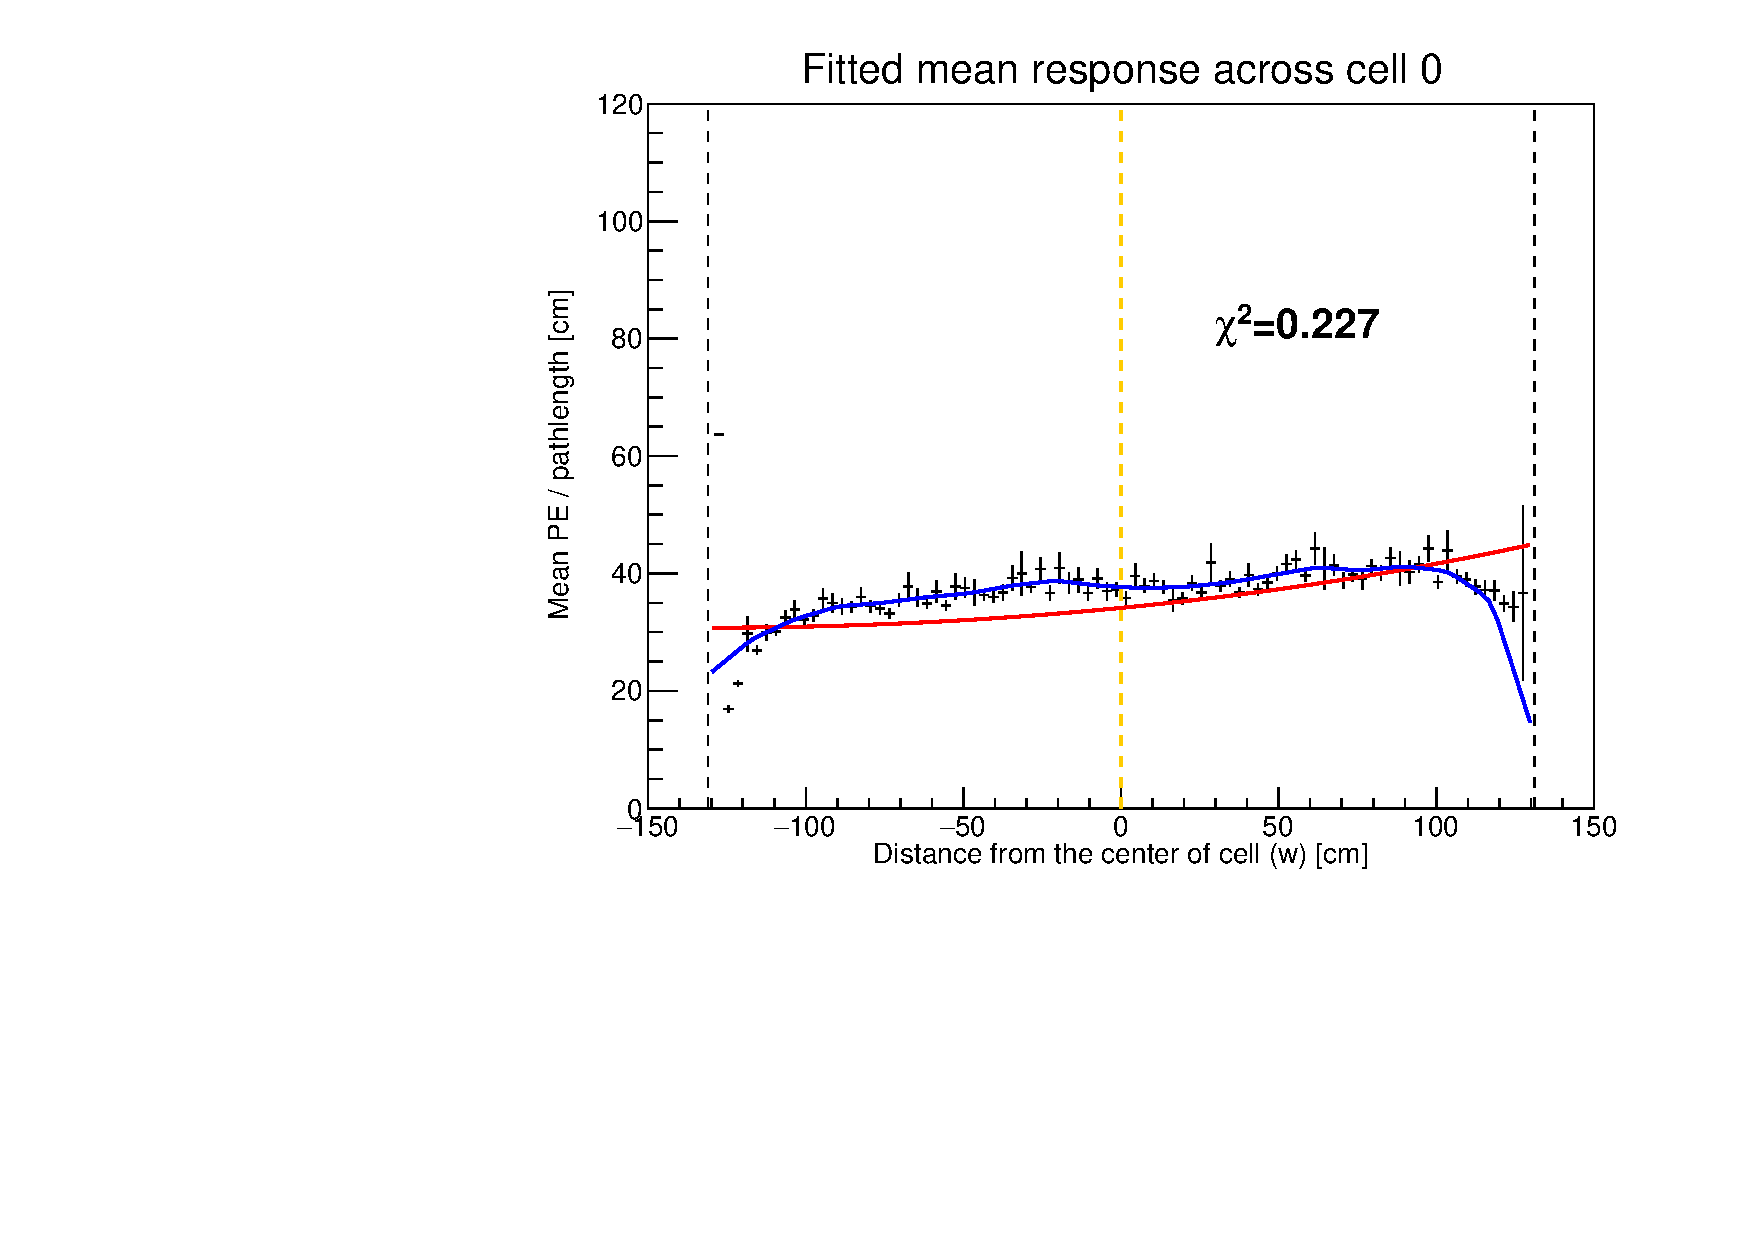
\includegraphics[width=\textwidth]{Plots/ExampleCellForFBFile_3000.pdf}
\end{subfigure}
%\hfill
\begin{subfigure}[b]{0.495\textwidth}
\centering
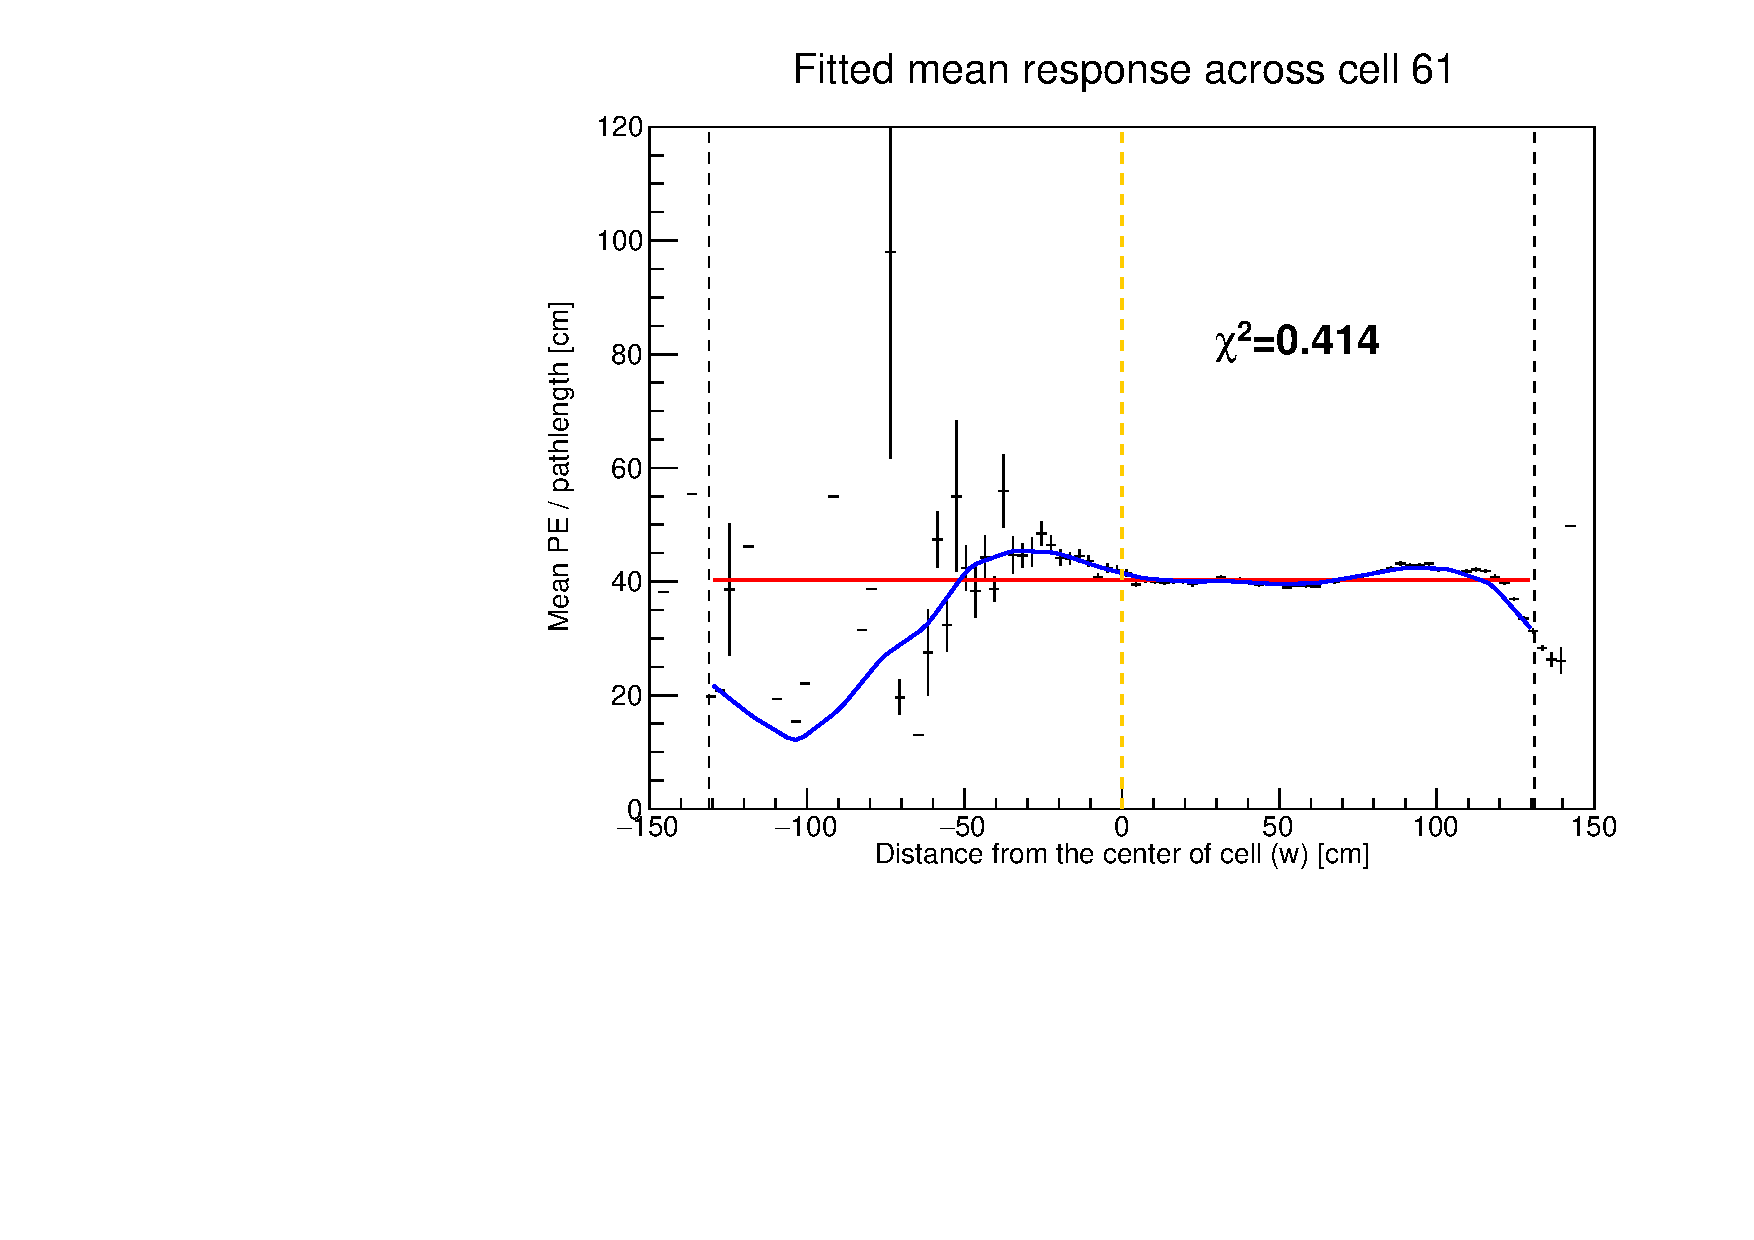
\includegraphics[width=\textwidth]{Plots/ExampleCellForFBFile_61061.pdf}
\end{subfigure}
\caption{Attenuation fits for two cells that fail the calibration condition, but the fit (blue line) correctly represents the energy deposition in the centre of that cell (yellow dashed line).}
\label{figFiberBrightnessExamples}
\end{figure}

The final distribution of brightness bins and their corresponding relative brightnesses for the Test Beam detector is shown on Fig. \ref{figFiberBrightnessBins}.

\subsection{Threshold and shielding corrections}
We created the threshold and shielding correction for Test Beam from the new simulation described in the next section \ref{secSimulationResults}. As can be seen on Fig. \ref{figTBThresholdCorrections}, the correction is almost uniform as a function of both $w$ and cell number. This is the case for all fibre brightness bins and for both views.

The uniform distribution is expected, as the Test Beam detector is much smaller than the far detector and the corrected effects don't have a significant effect. The cell length of $2.6\ \unit{m}$ has only a negligible effect on the energy distribution of cosmic muons or on the threshold saturation. Therefore the threshold and shielding correction for Test Beam is only a normalization factor, except for the cell edges, where there is a large variation in the energy response there anyway due to low number of events. Since the relative calibration only cares about relative differences across the detector, a normalization factor does not have any impact on its results.

\begin{figure}[hbtp]
\centering
\begin{subfigure}[t]{0.9\textwidth}
\centering
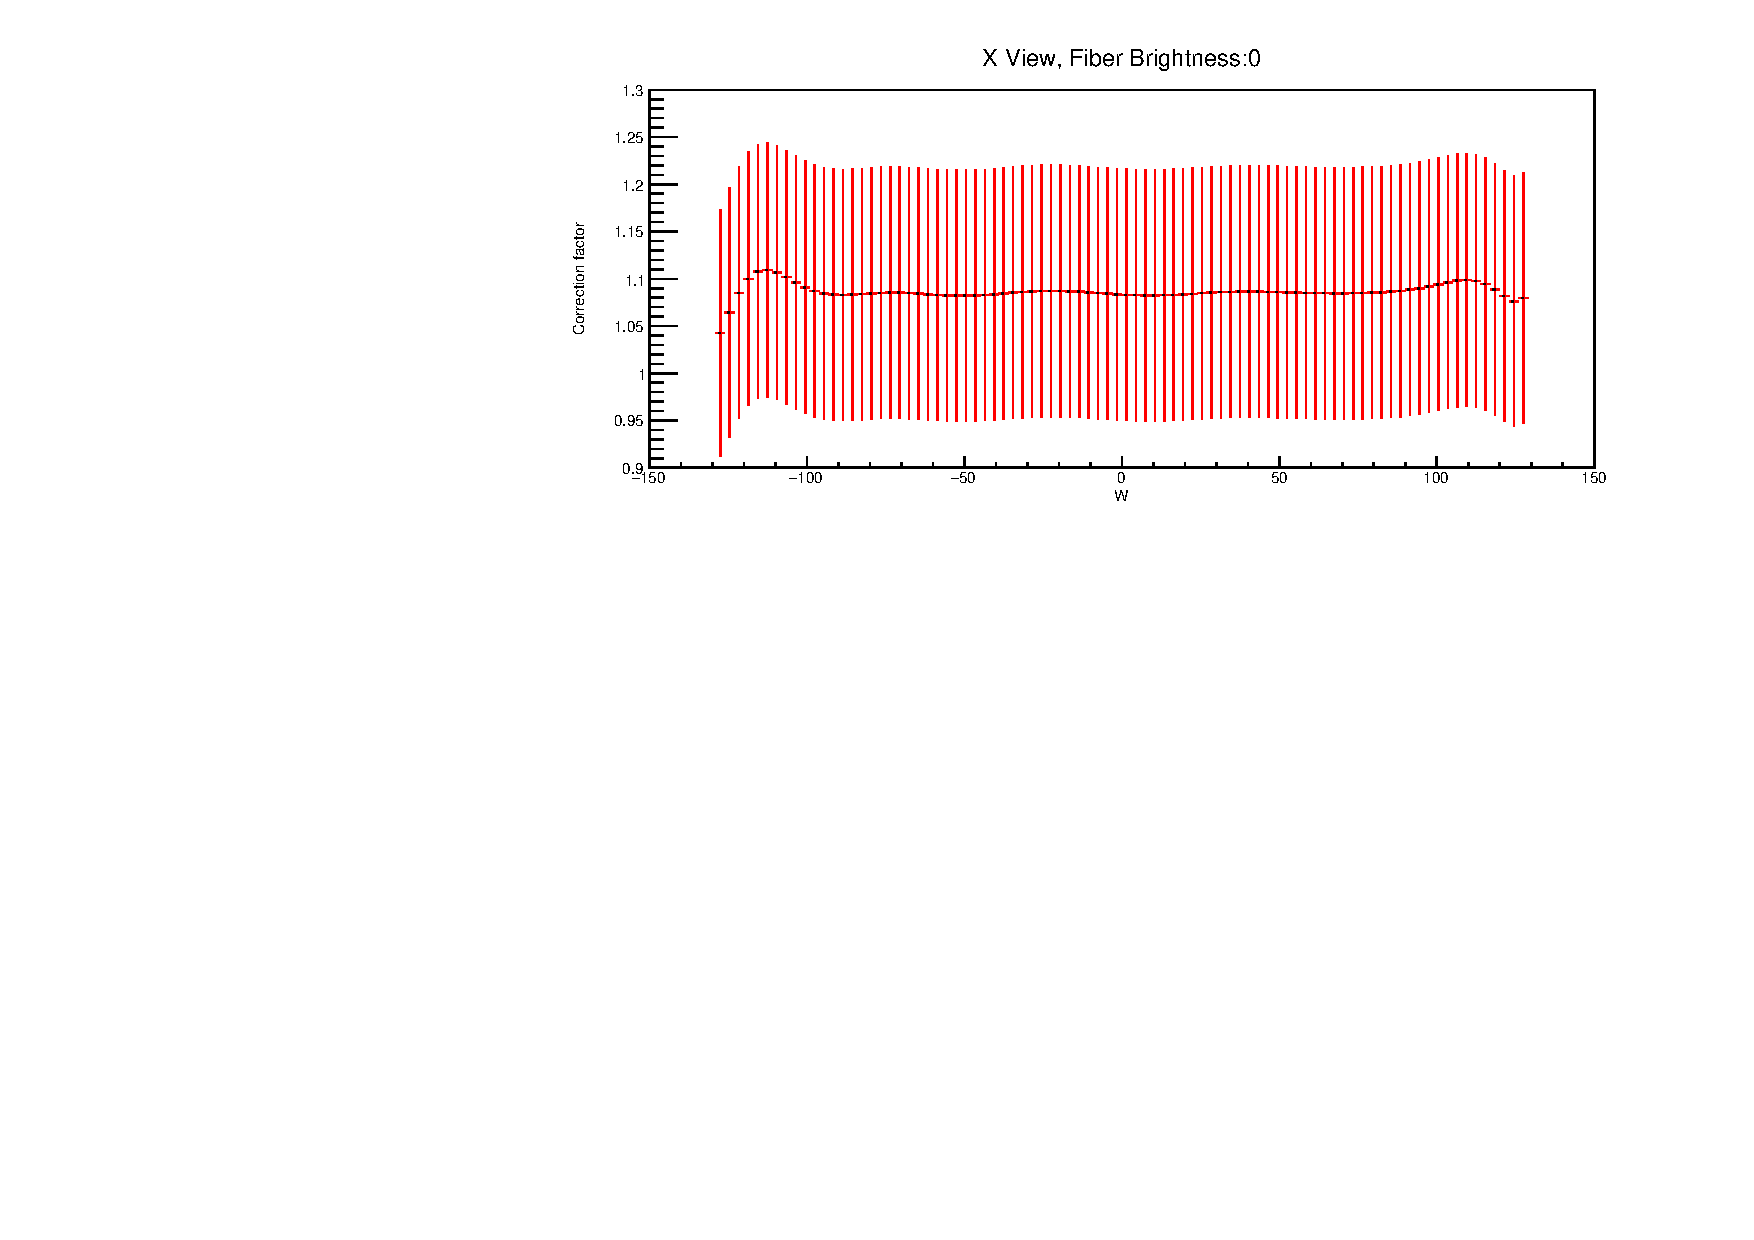
\includegraphics[width=\textwidth]{Plots/ThresholdCorrectionExample_axview_fb0_P4DataBasedSim.pdf}
\end{subfigure}
\begin{subfigure}[b]{0.9\textwidth}
\centering
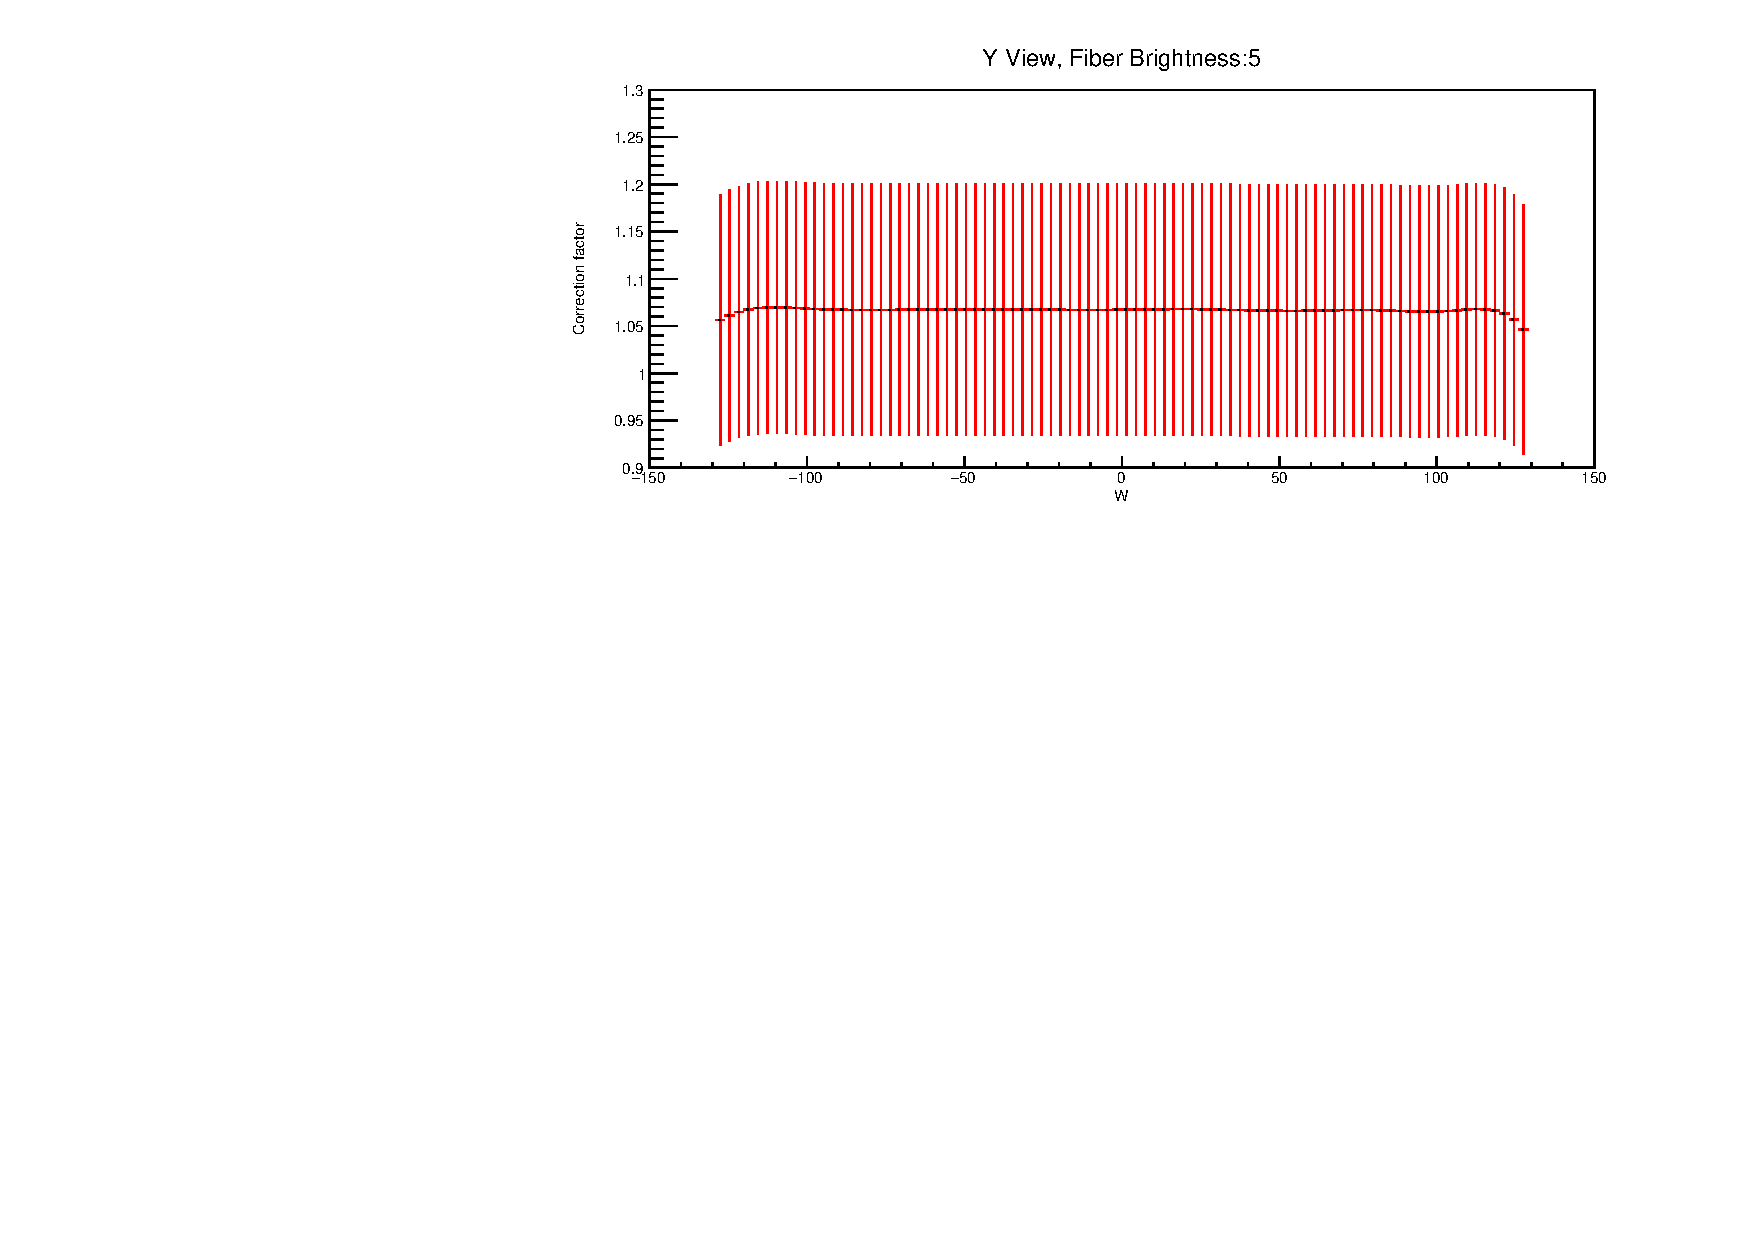
\includegraphics[width=\textwidth]{Plots/ThresholdCorrectionExample_ayview_fb5_P4DataBasedSim.pdf}
\end{subfigure}
\begin{subfigure}[t]{0.9\textwidth}
\centering
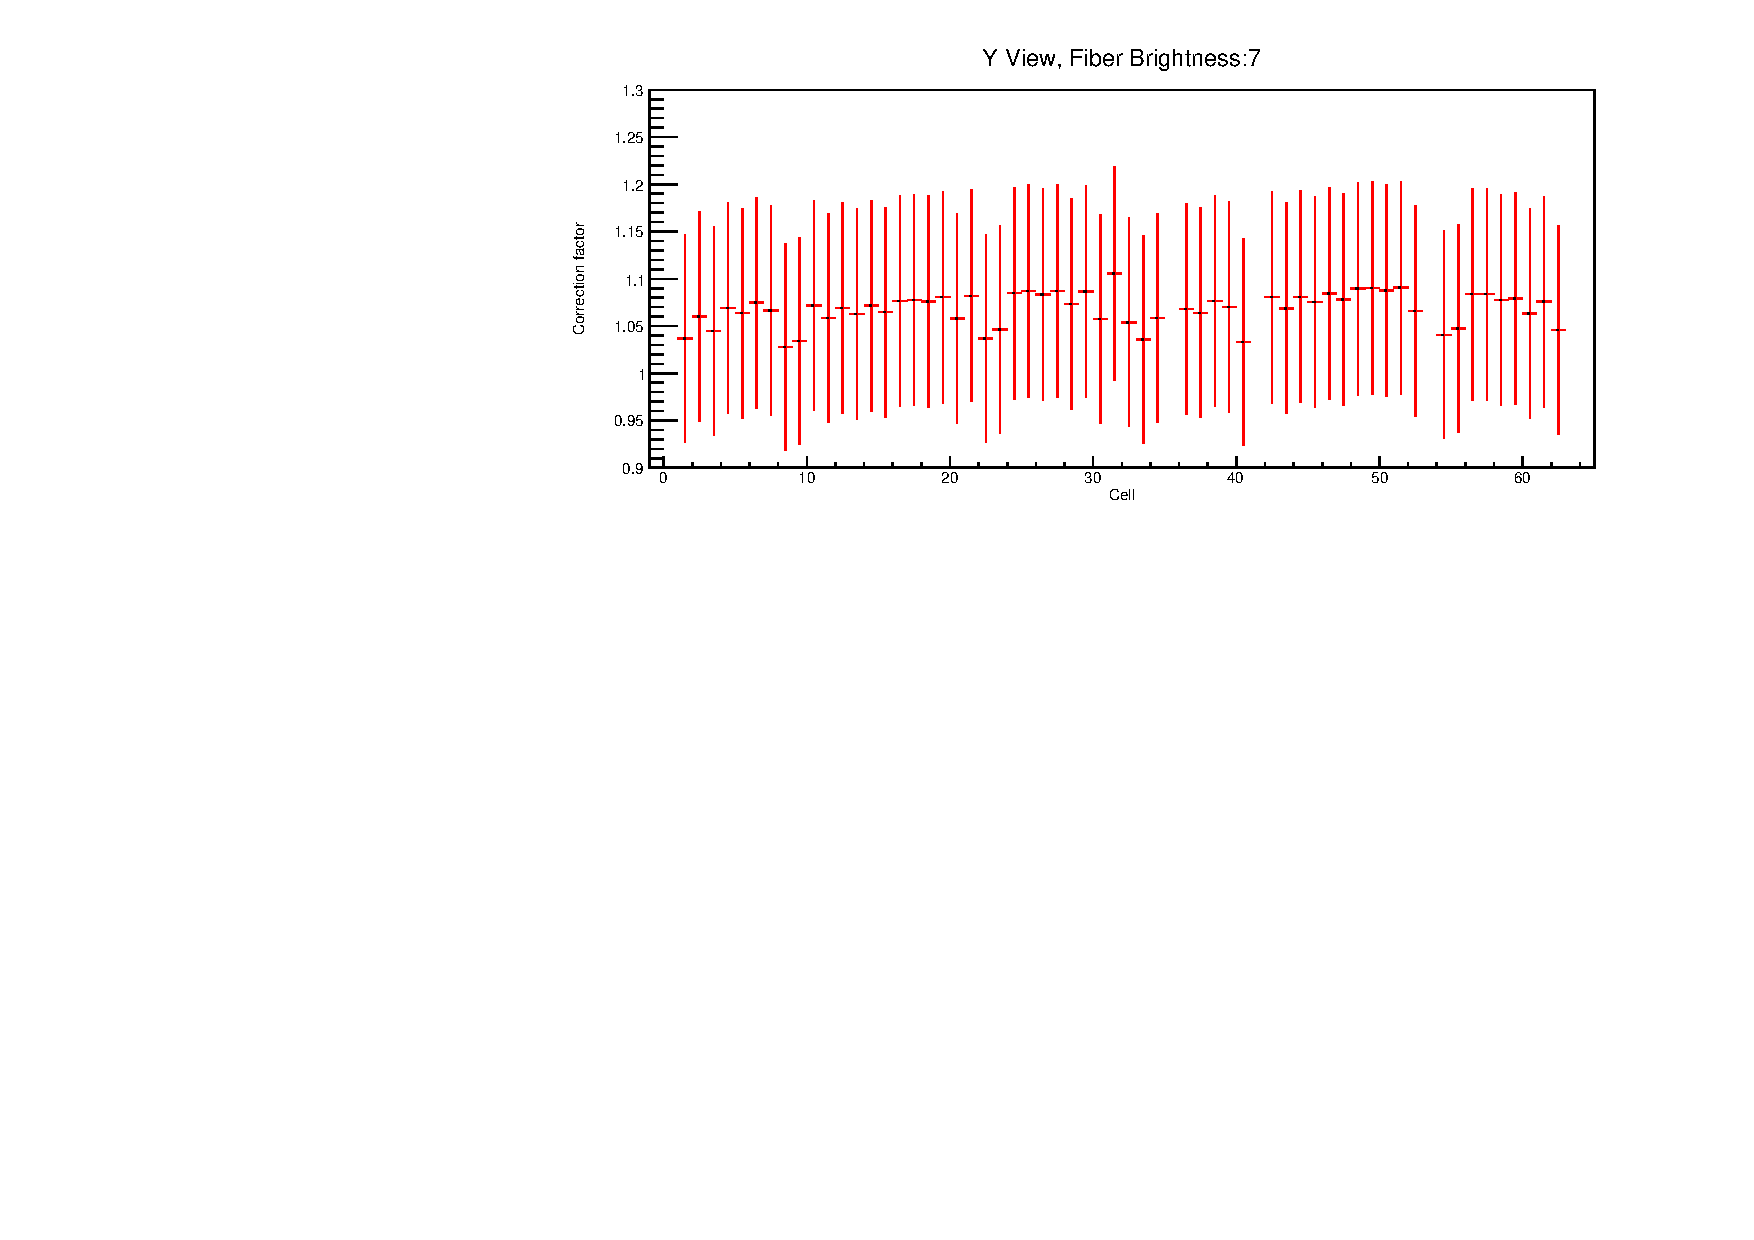
\includegraphics[width=\textwidth]{Plots/ThresholdCorrectionExample_cyview_fb7_P4DataBasedSim.pdf}
\end{subfigure}
\caption{Examples of threshold and shielding corrections for the Test Beam detector}
\label{figTBThresholdCorrections}
\end{figure}

\subsection{Simulation}\label{secSimulationResults}

%Should I talk about the "history" of the simulation of cosmics here, or in the introduction, or not at all?

%We originally used Teresa's calibration MC sample, but after we saw disagreement, we developed a new MC based off of the period 3 data, which we ended up using for both period 2 and period 3. For fibre brightness we are also using the same MC from period 3 data as it represents the detector in its best condition.

We used a custom made data-based simulation of cosmic muons for the Test Beam detector calibration. The details on the simulation and how it was created are described in the \textit{"Data-based simulation of cosmic muons (not only) for calibration technical note"} \cite{NOVA-doc-60026}. We used half of period 4 data (used every second event as saved in the root file, therefore sampled from the entire period 4) as the inputs. We also used the newly created fibre brightness file (section\ref{secFibreBrightnessTB}) to inform the simulation on the realistic detector conditions.

The distribution of cosmic muon events from the new simulation across the detector is shown on Fig. \ref{figCalibhistSim}.

\begin{figure}[h]
\centering
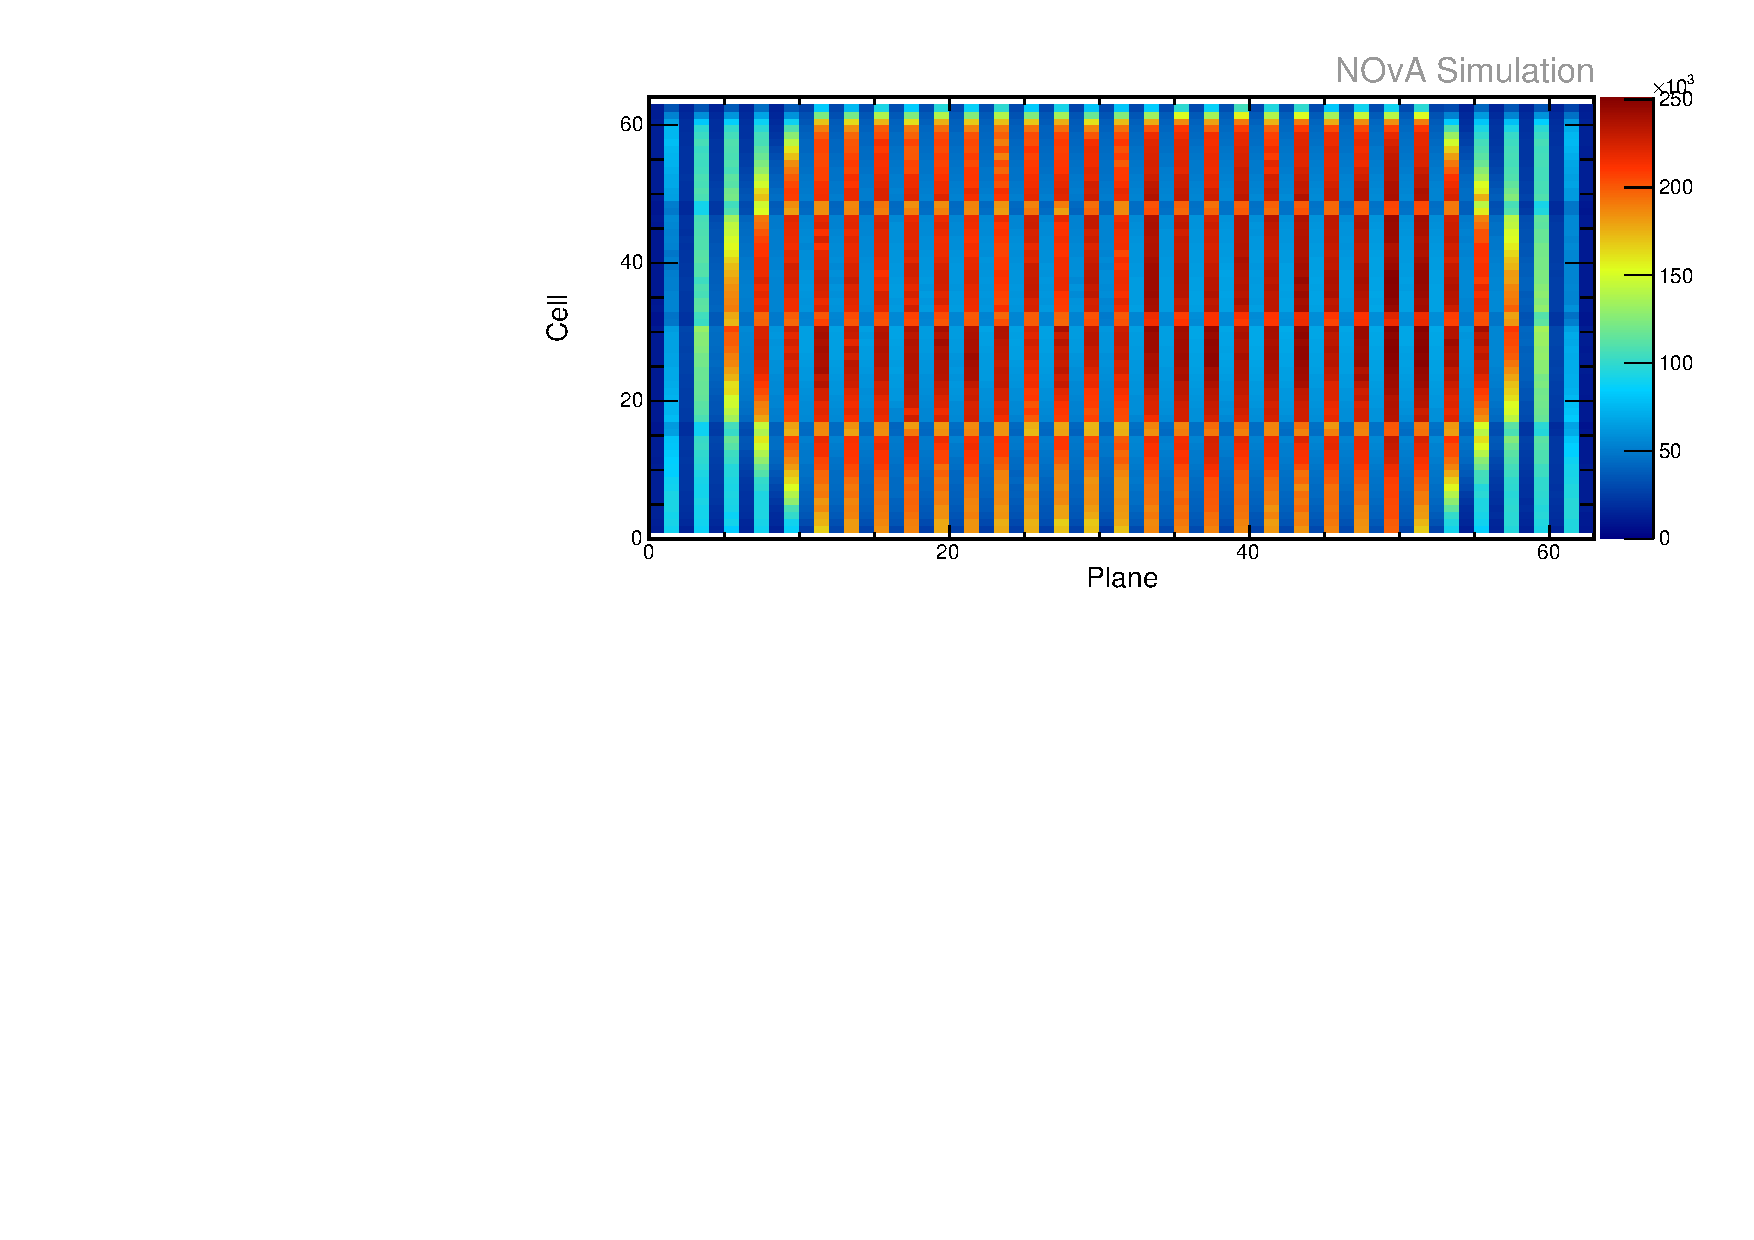
\includegraphics[width=.9\textwidth]{Plots/Attenprofs_Simulation_CellPlane.pdf}
\caption{Distribution of events in the Test Beam simulation calibration sample.}
\label{figCalibhistSim}
\end{figure}

An overview of the results of the attenuation fit are shown on Fig. \ref{figCellCentreResponseSim} as a map of the response in the centre of each cell. The blank cells show the uncalibrated cells which failed the calibration condition (attenuation fit $\chi^2>0.2$). Most of the uncalibrated cells are on the edges of the detector, which is expected as those have much fewer events that pass the calibration sample selection than the rest.

Examples of a standard detector response and of the response for cells on the edge of the detector are shown of Fig. \ref{figAttenfitResultsSimulation}. Here the red line shows the initial exponential fit and the blue line the final attenuation fit, after the LOWESS correction, as described in section \ref{secRelativCalibration}. Most cells have an expected response with a slow rise towards the readout (right side of the plots), with drops on the edges, as shown on the top left plot.

\begin{figure}[h]
\centering
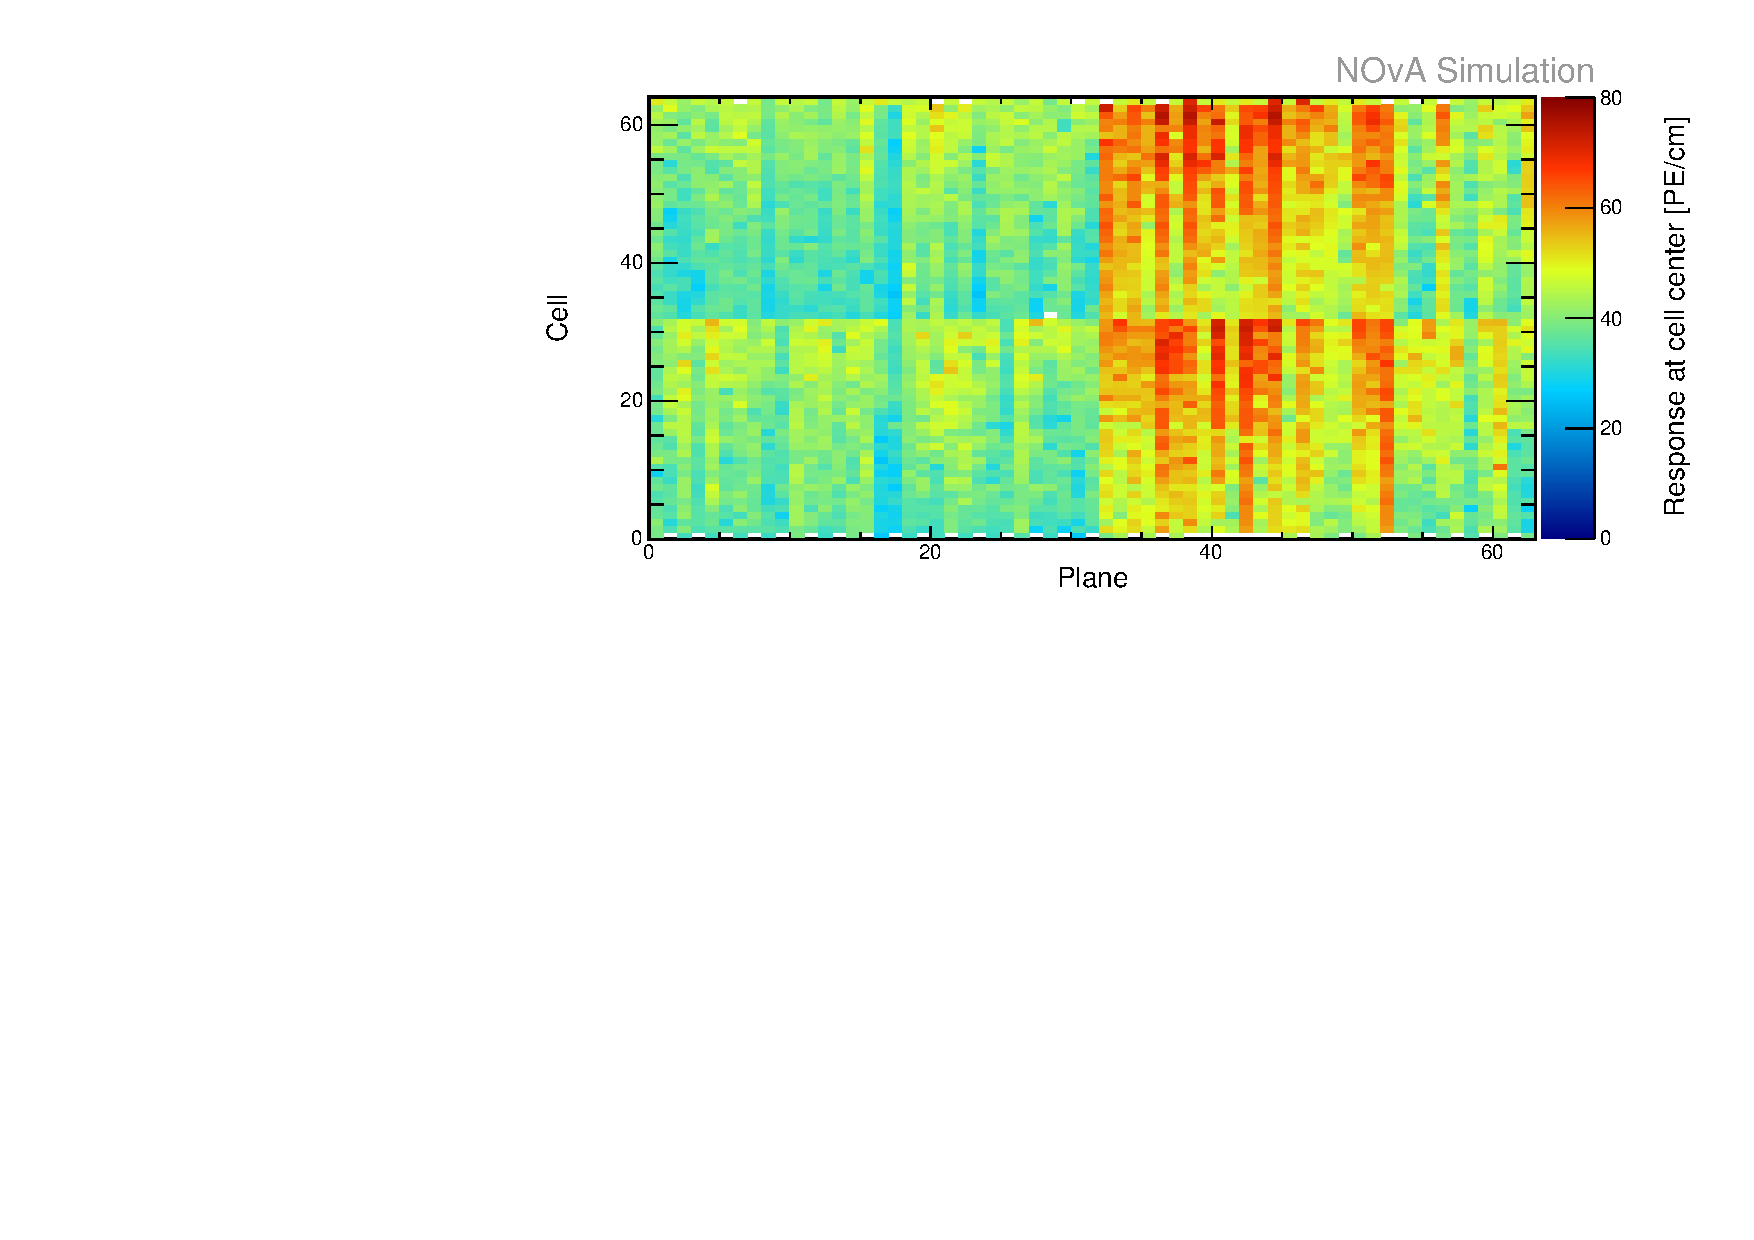
\includegraphics[width=\textwidth]{Plots/CellResponseAtCentre_Prod4DataBasedSim_Limited_NOvAPlotStyle.pdf}
\caption{Overview of the attenuation fit results for the Test Beam detector calibration simulation. Each cell represents the result of the attenuation fit to the energy response in the centre of that cell. The blank cells are uncalibrated.}
\label{figCellCentreResponseSim}
\end{figure}

There is only one cell in the middle of the detector that is left uncalibrated, which is the cell 32 in a vertical plane in the brightness bin 5, shown on the top right of Fig.\ref{figAttenfitResultsSimulation}. The corresponding $\chi^2=0.227$. It seems the reason the $\chi^2$ is $>0.2$ is the high response with a large uncertainty in the very last fitted bin.

\begin{figure}[h]
  \begin{subfigure}{0.5\textwidth}
    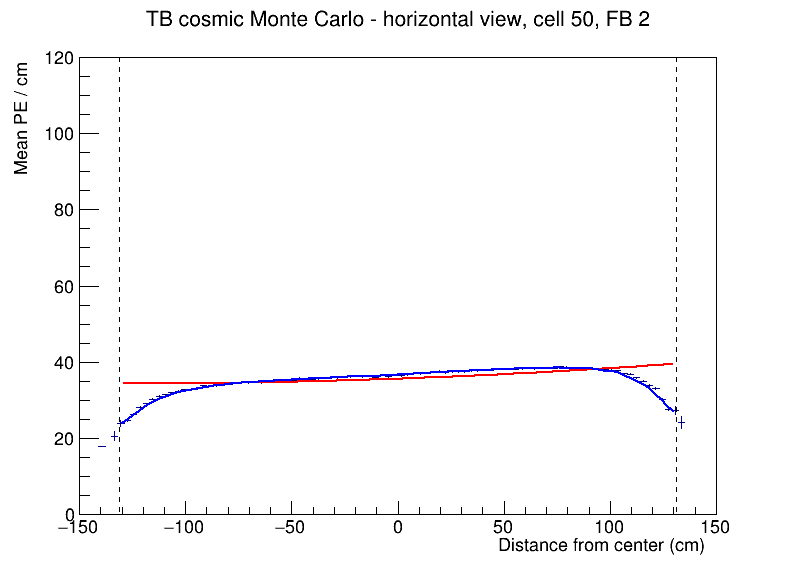
\includegraphics[width=\linewidth]{RelativeCalibrationResults/sim_fb2_001_050.png}
  \end{subfigure}
  \begin{subfigure}{0.5\textwidth}
    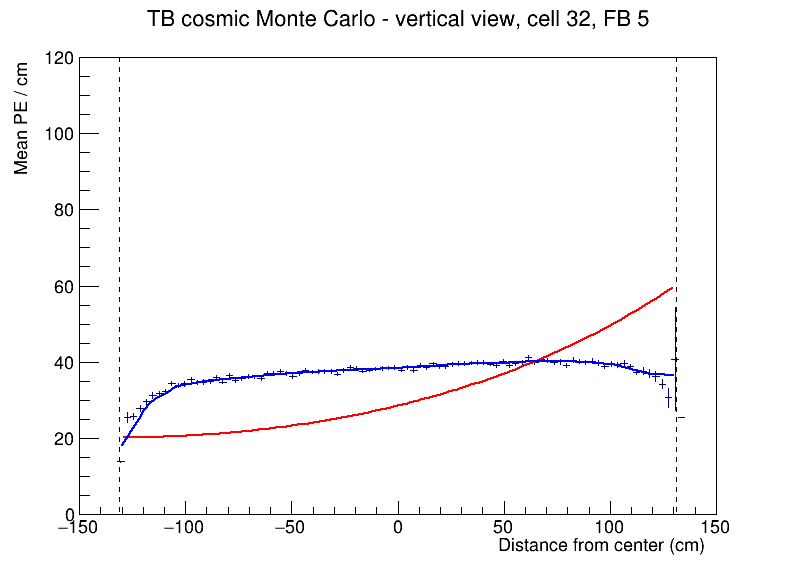
\includegraphics[width=\linewidth]{RelativeCalibrationResults/sim_fb5_000_032.png}
  \end{subfigure}
  \begin{subfigure}{0.5\textwidth}
    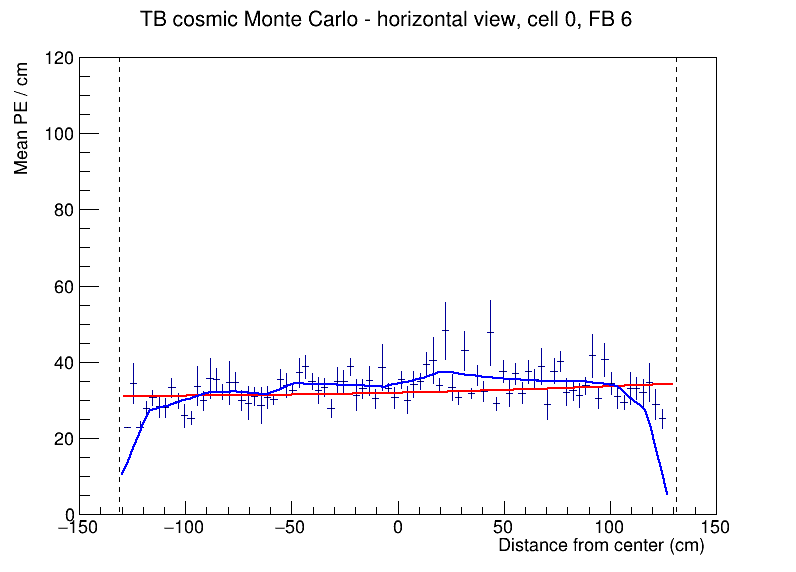
\includegraphics[width=\linewidth]{RelativeCalibrationResults/sim_fb6_001_000.png}
  \end{subfigure}
  \begin{subfigure}{0.5\textwidth}
    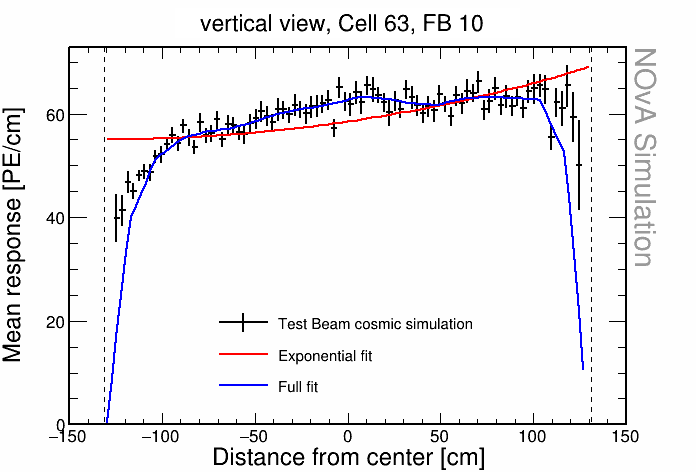
\includegraphics[width=\linewidth]{RelativeCalibrationResults/sim_fb10_000_063.png}
  \end{subfigure}
  \caption{Attenuation fits for a selection of cells in the Test Beam calibration simulation. Top left is an example of a successful attenuation fit, top right is a failed fit due to statistical fluctuation in the last bin and the bottom plots show failed fits for cells on the edges of the detector.}
  \label{figAttenfitResultsSimulation}
\end{figure}

Overall, this is a much better result of the relative calibration (attenuation fit) for a simulation than any of the previous versions of the cosmic muon simulations in the Test Beam detector.

\FloatBarrier
\subsection{Period 2 data}
The issue with underfilled cells described in section \ref{secTBDetector} was present throughout the period 2 data taking. This can be clearly seen on Fig. \ref{figCalibhist_period2}, represented by the empty cells 31 and 63 in the horizontal planes, which were marked as bad channels and therefore ignored during production of calibration samples. This also affects the neighbouring cells to the underfilled cells, which have fewer events due to the tricell condition (see section \ref{secCreatingCalibrationSamples}).

\begin{figure}[h]
\centering
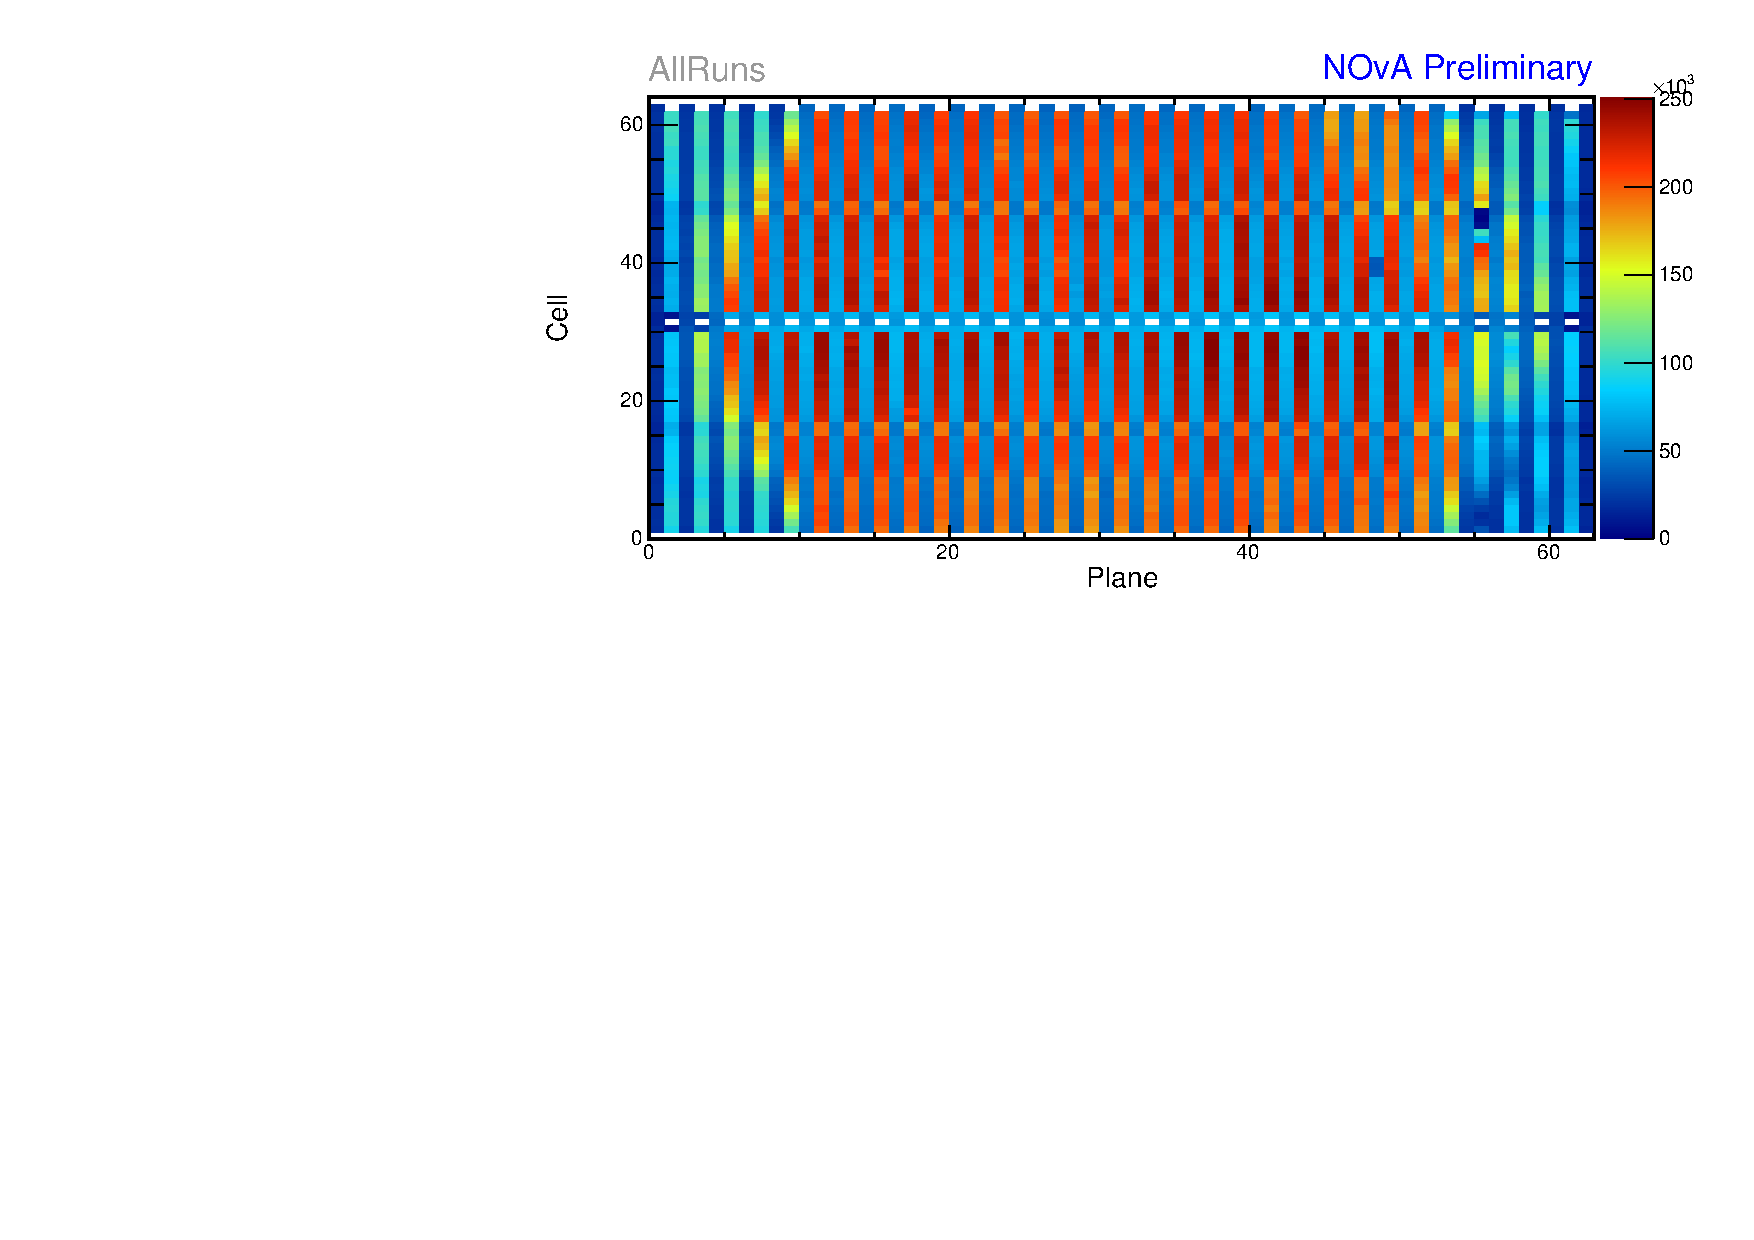
\includegraphics[width=0.9\textwidth]{Plots/Attenprofs_P2Data_CellPlane_AllRuns.pdf}
\caption{Distribution of events in the period 2 Test Beam data calibration sample.}
\label{figCalibhist_period2}
\end{figure}

There was also an issue of likely switched cables from the readout in plane 55 between cells 3 and 46 \cite{NOVA-doc-49674}, which can also be seen on Fig. \ref{figCalibhist_period2} as dark spots. This is manifested as fewer total number of events in those cells and in their neighbours, again due to the tricell condition.

Officially, period 2 is divided into 6 epochs 2a - 2f, compared on figures \ref{figCalibhistWPE_period2},\ref{figCalibhistCellPE_period2} and \ref{figCalibhistPlanePE_period2}. The epochs mostly differ in the use of various FEB firmwares, with epoch 2c being a trigger study with paddles. As can be seen on the plots, the individual epochs vary only slightly, and only in a small normalization difference. We decided to calibrate the entire period 2 together, without splitting it into any smaller samples.

\begin{figure}[h]
\centering
\begin{subfigure}[b]{0.495\textwidth}
\centering
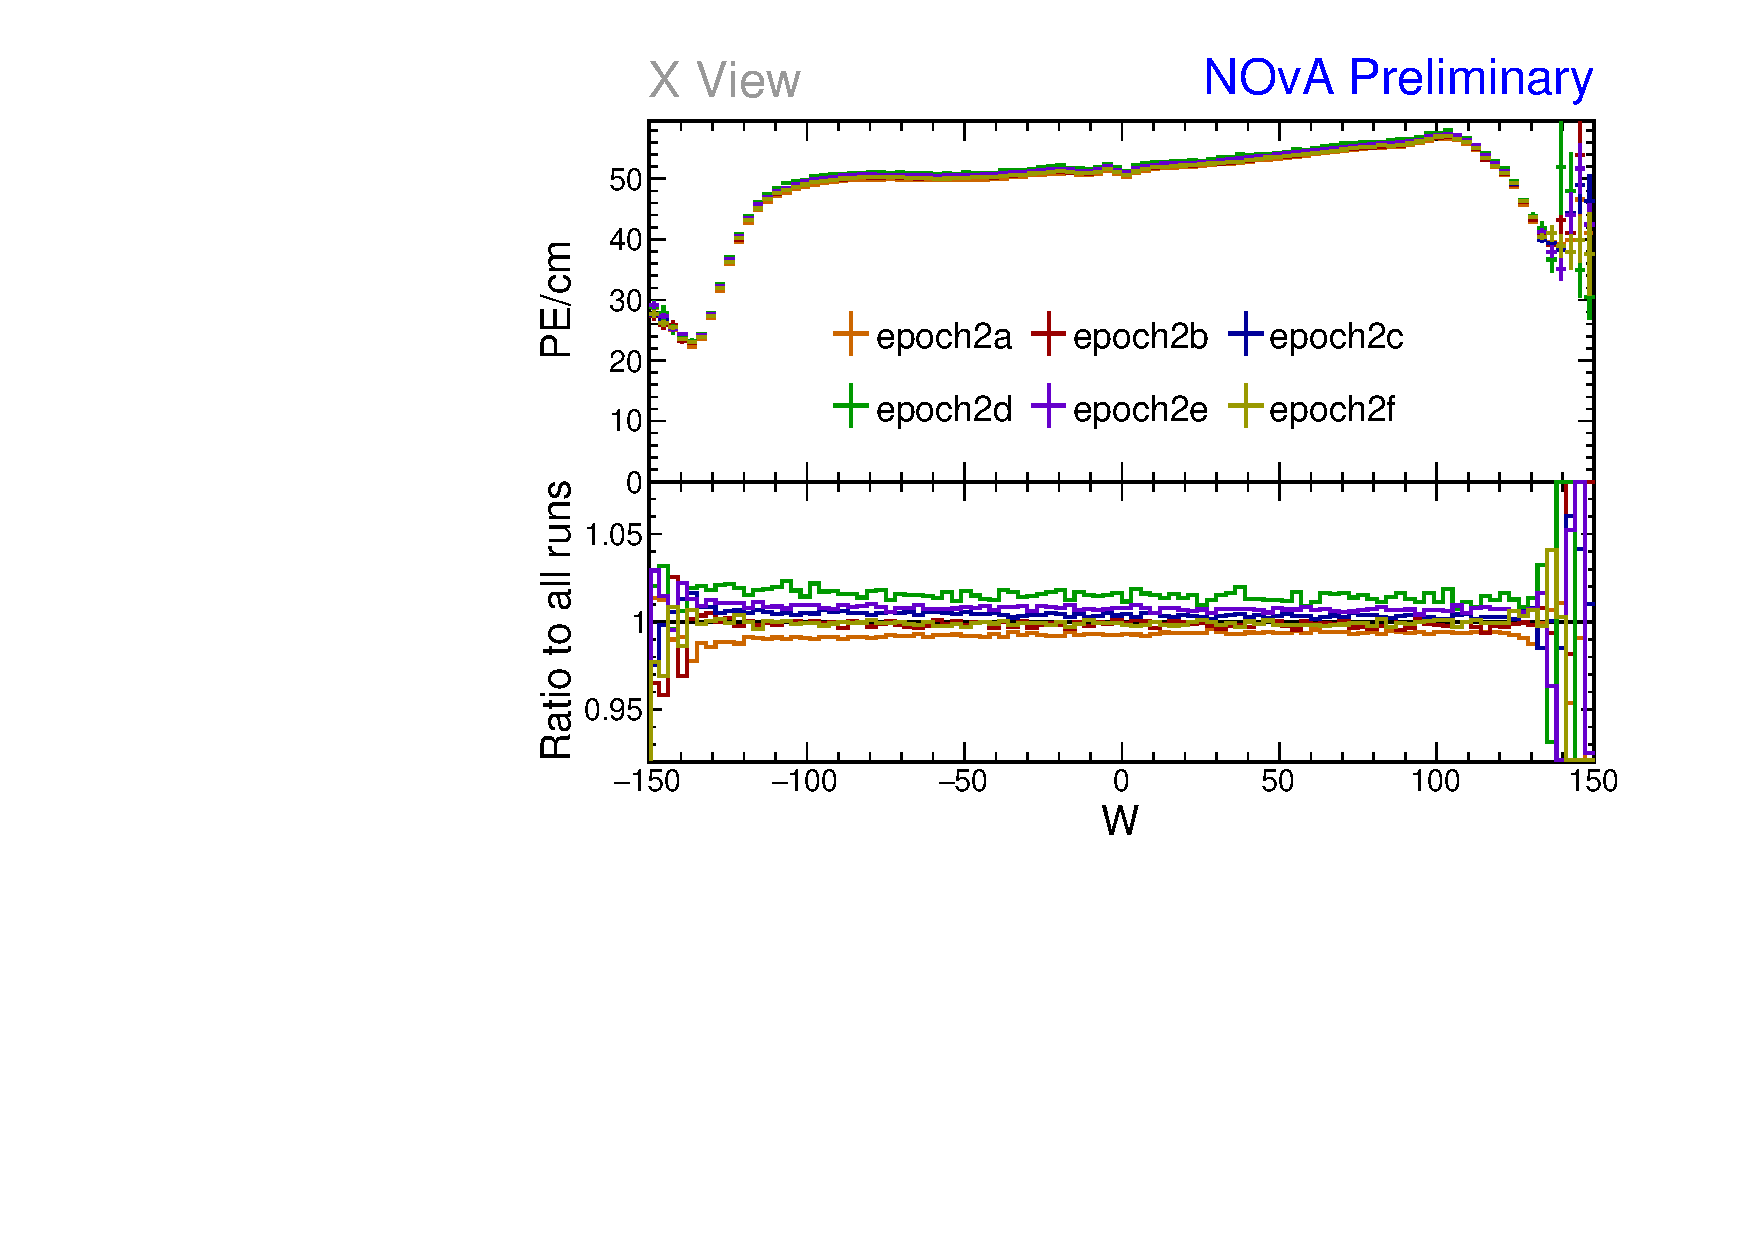
\includegraphics[width=\textwidth]{Plots/Attenprofs_P2Data_WPE_corr_xy_X_Combined.pdf}
\end{subfigure}
\begin{subfigure}[b]{0.495\textwidth}
\centering
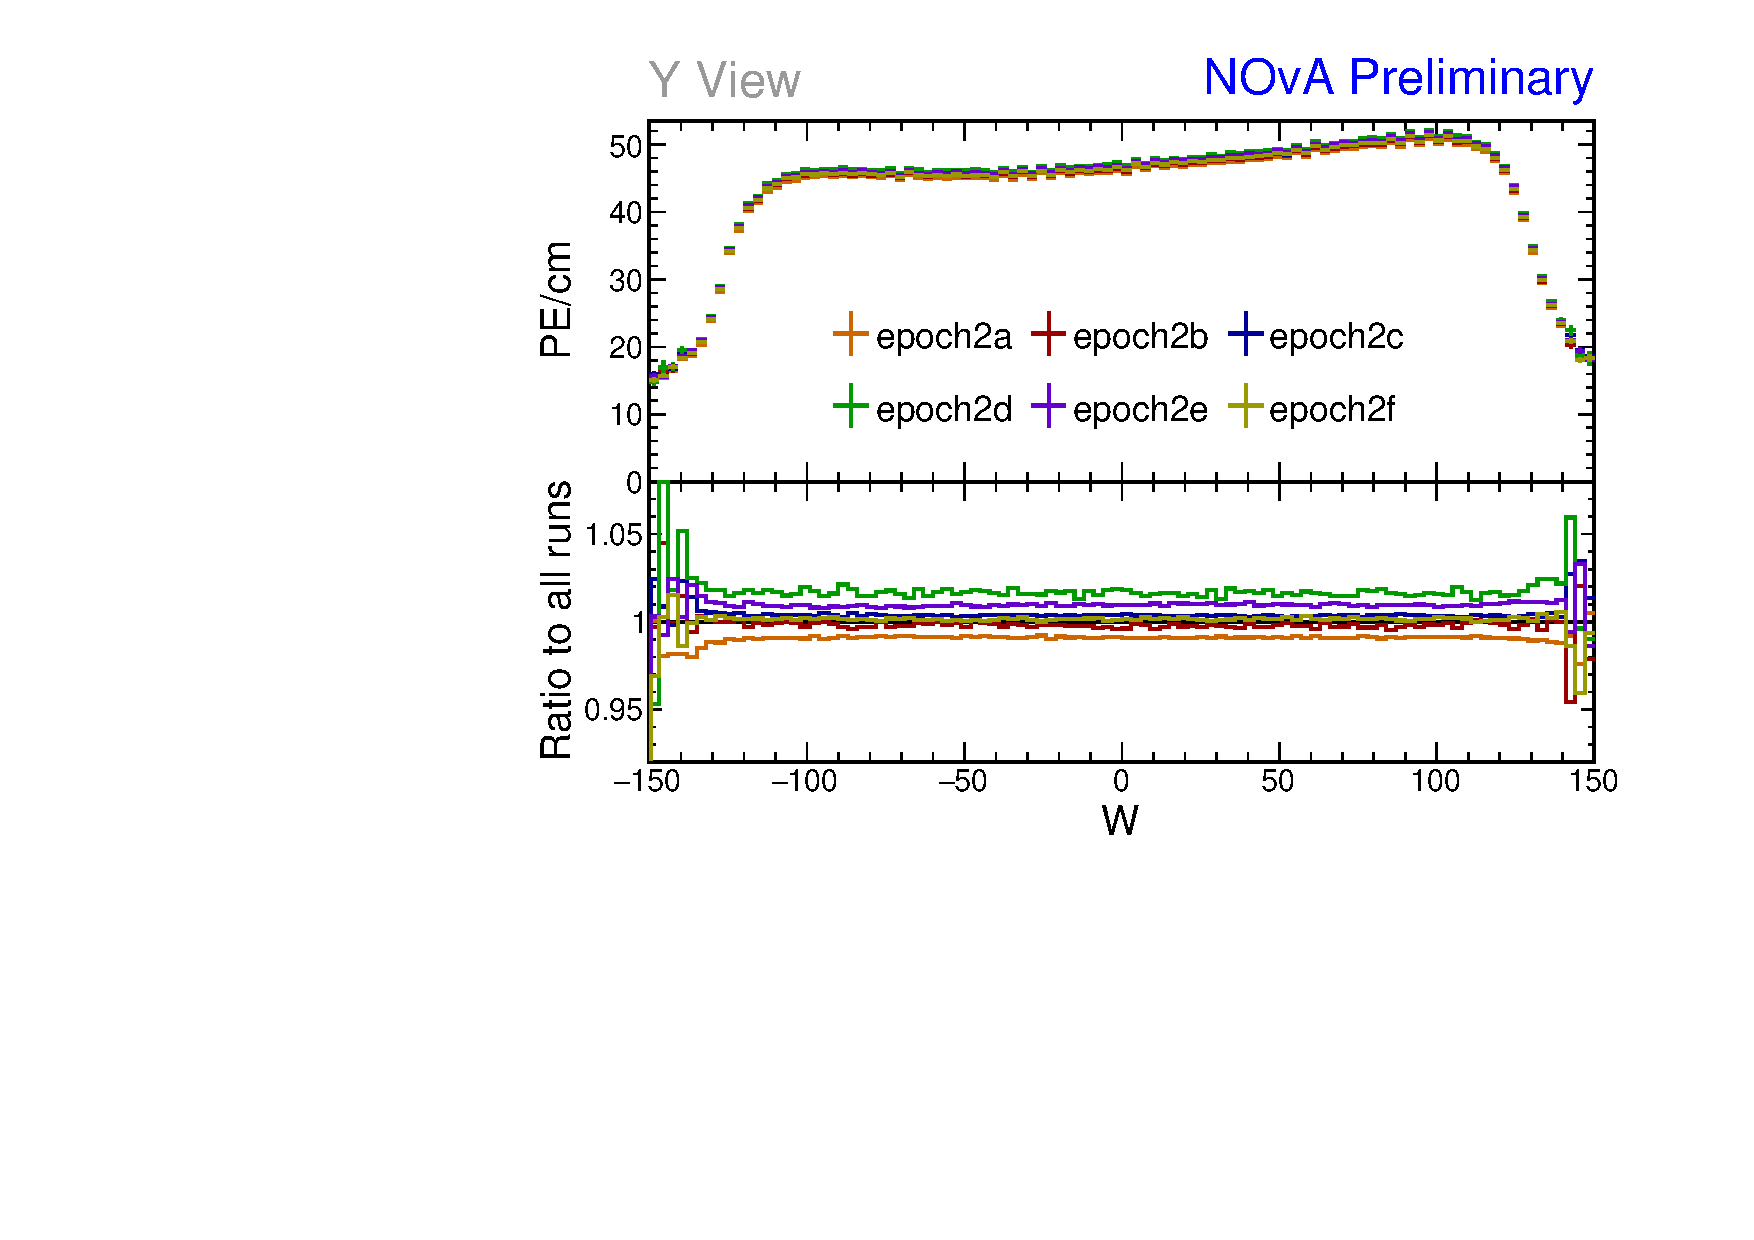
\includegraphics[width=\textwidth]{Plots/Attenprofs_P2Data_WPE_corr_xy_Y_Combined.pdf}
\end{subfigure}
\caption{Uncorrected average energy response as a function of the position within a cell (w) for epochs in period 2. It is clear that there is no significant difference between the various epochs.}
\label{figCalibhistWPE_period2}
\end{figure}

\begin{figure}[h]
\centering
\begin{subfigure}[b]{0.495\textwidth}
\centering
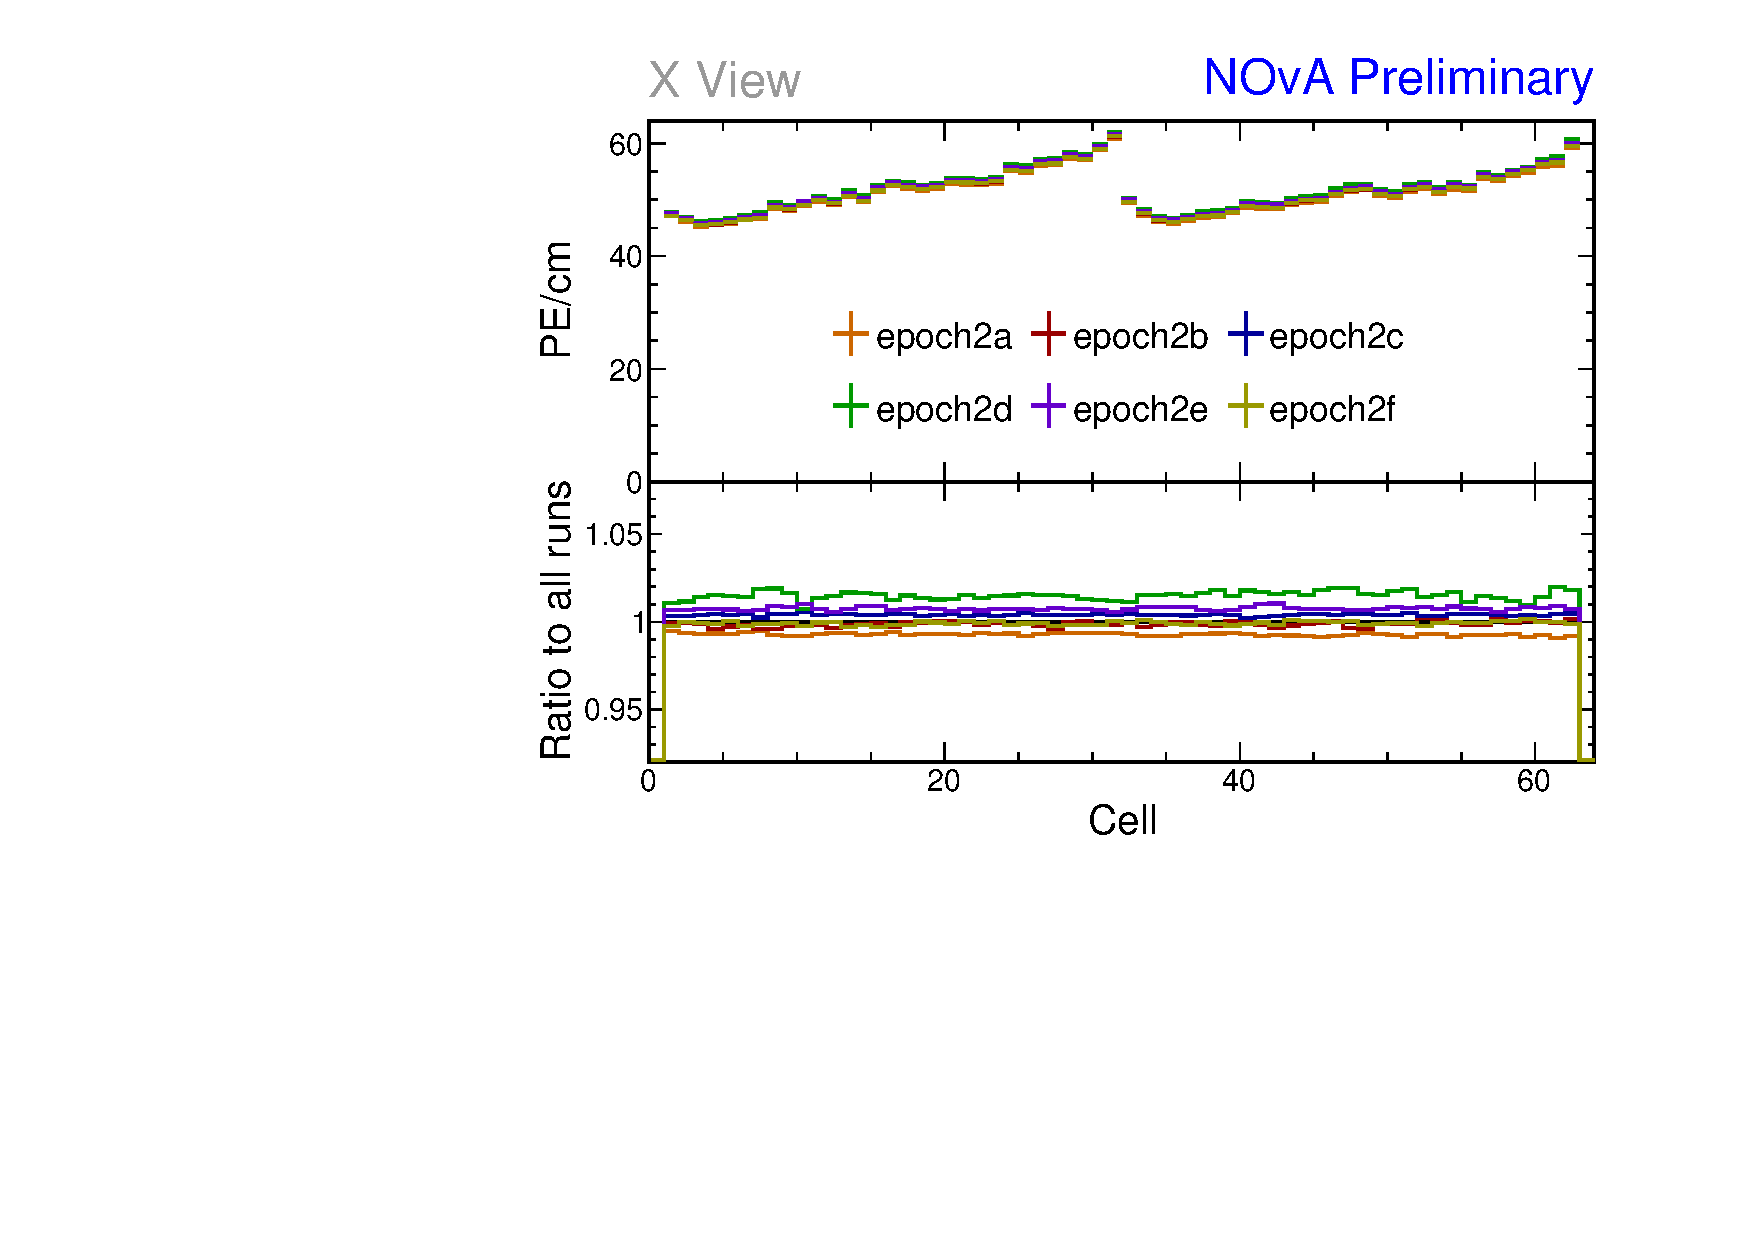
\includegraphics[width=\textwidth]{Plots/Attenprofs_P2Data_CellPE_X_Combined.pdf}
\end{subfigure}
\begin{subfigure}[b]{0.495\textwidth}
\centering
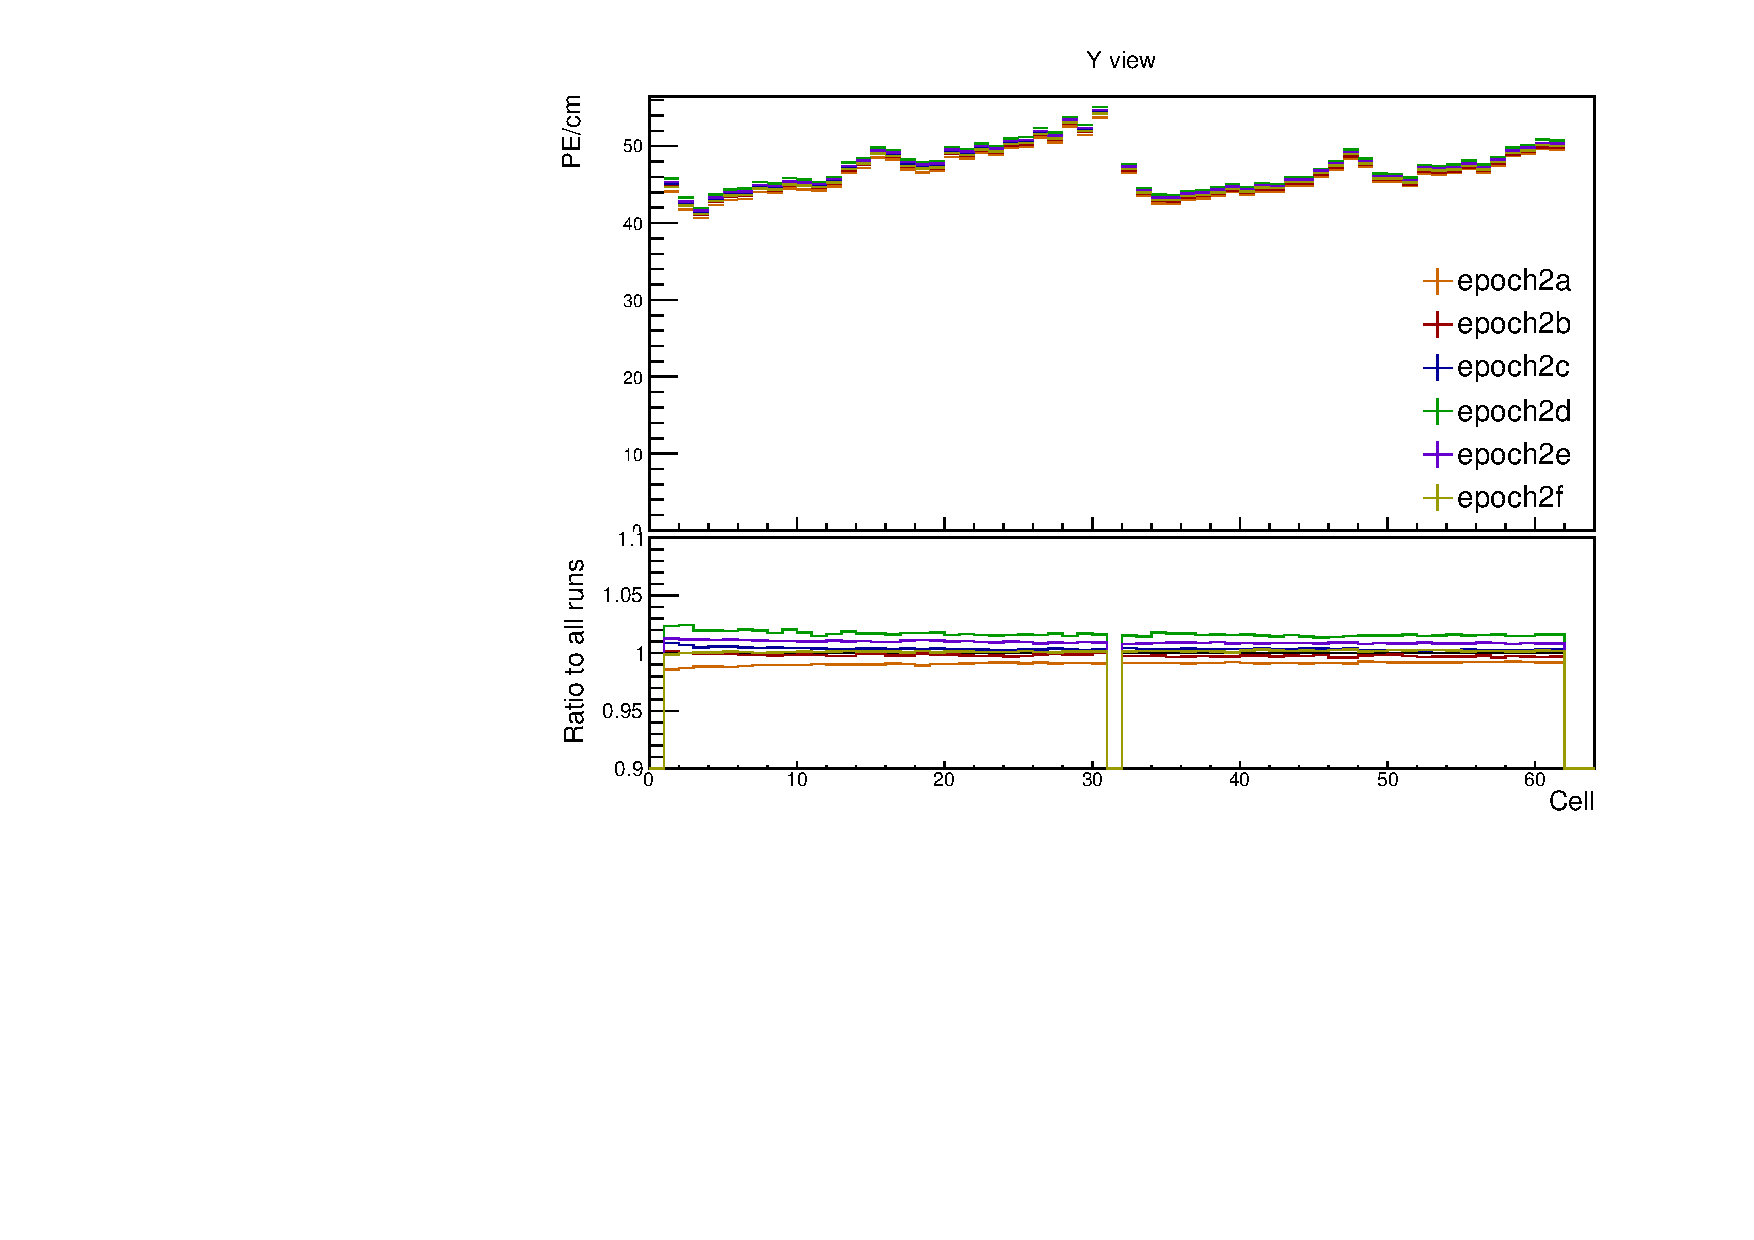
\includegraphics[width=\textwidth]{Plots/Attenprofs_P2Data_CellPE_Y_Combined.pdf}
\end{subfigure}
\caption{Uncorrected average energy response as a function of cells for epochs in period 2.}
\label{figCalibhistCellPE_period2}
\end{figure}

\begin{figure}[h]
\centering
\begin{subfigure}[b]{0.495\textwidth}
\centering
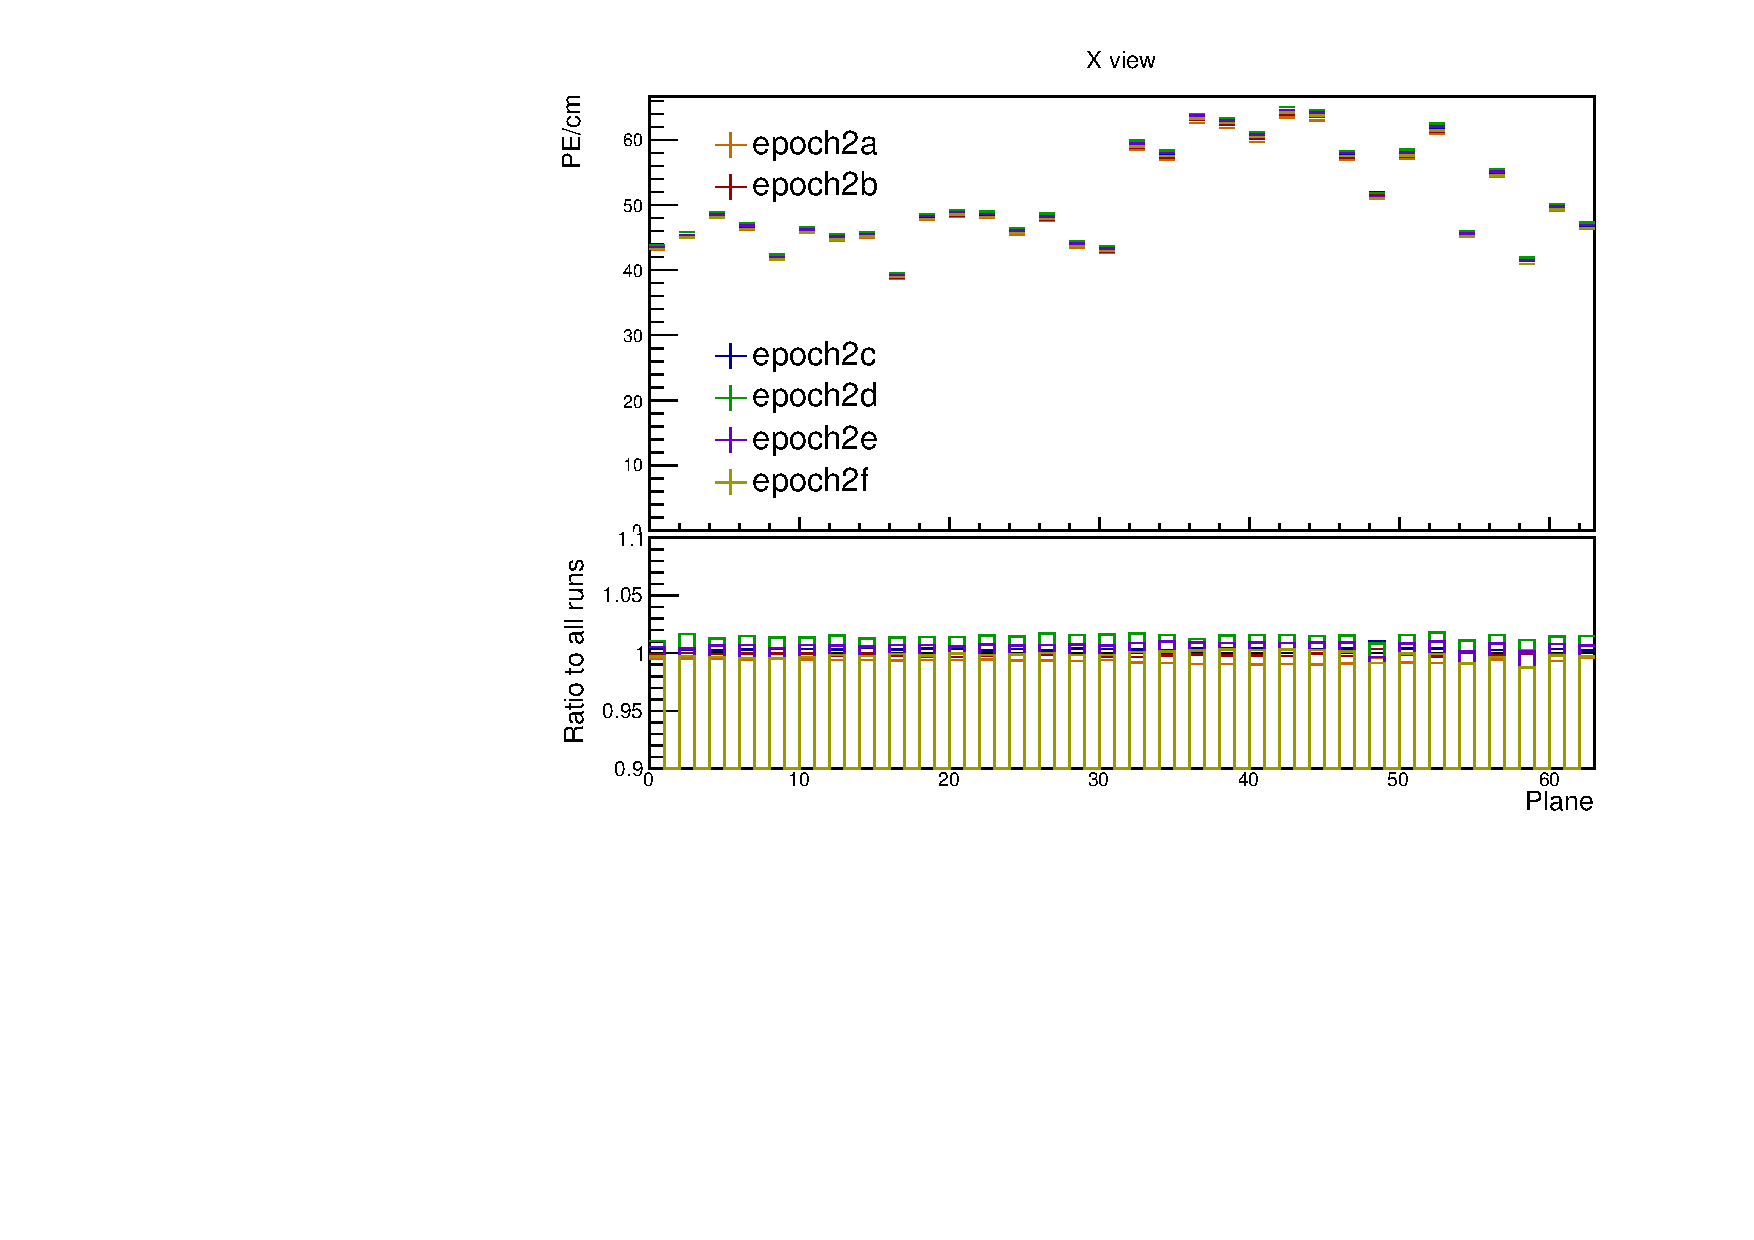
\includegraphics[width=\textwidth]{Plots/Attenprofs_P2Data_PlanePE_X_Combined.pdf}
\end{subfigure}
\begin{subfigure}[b]{0.495\textwidth}
\centering
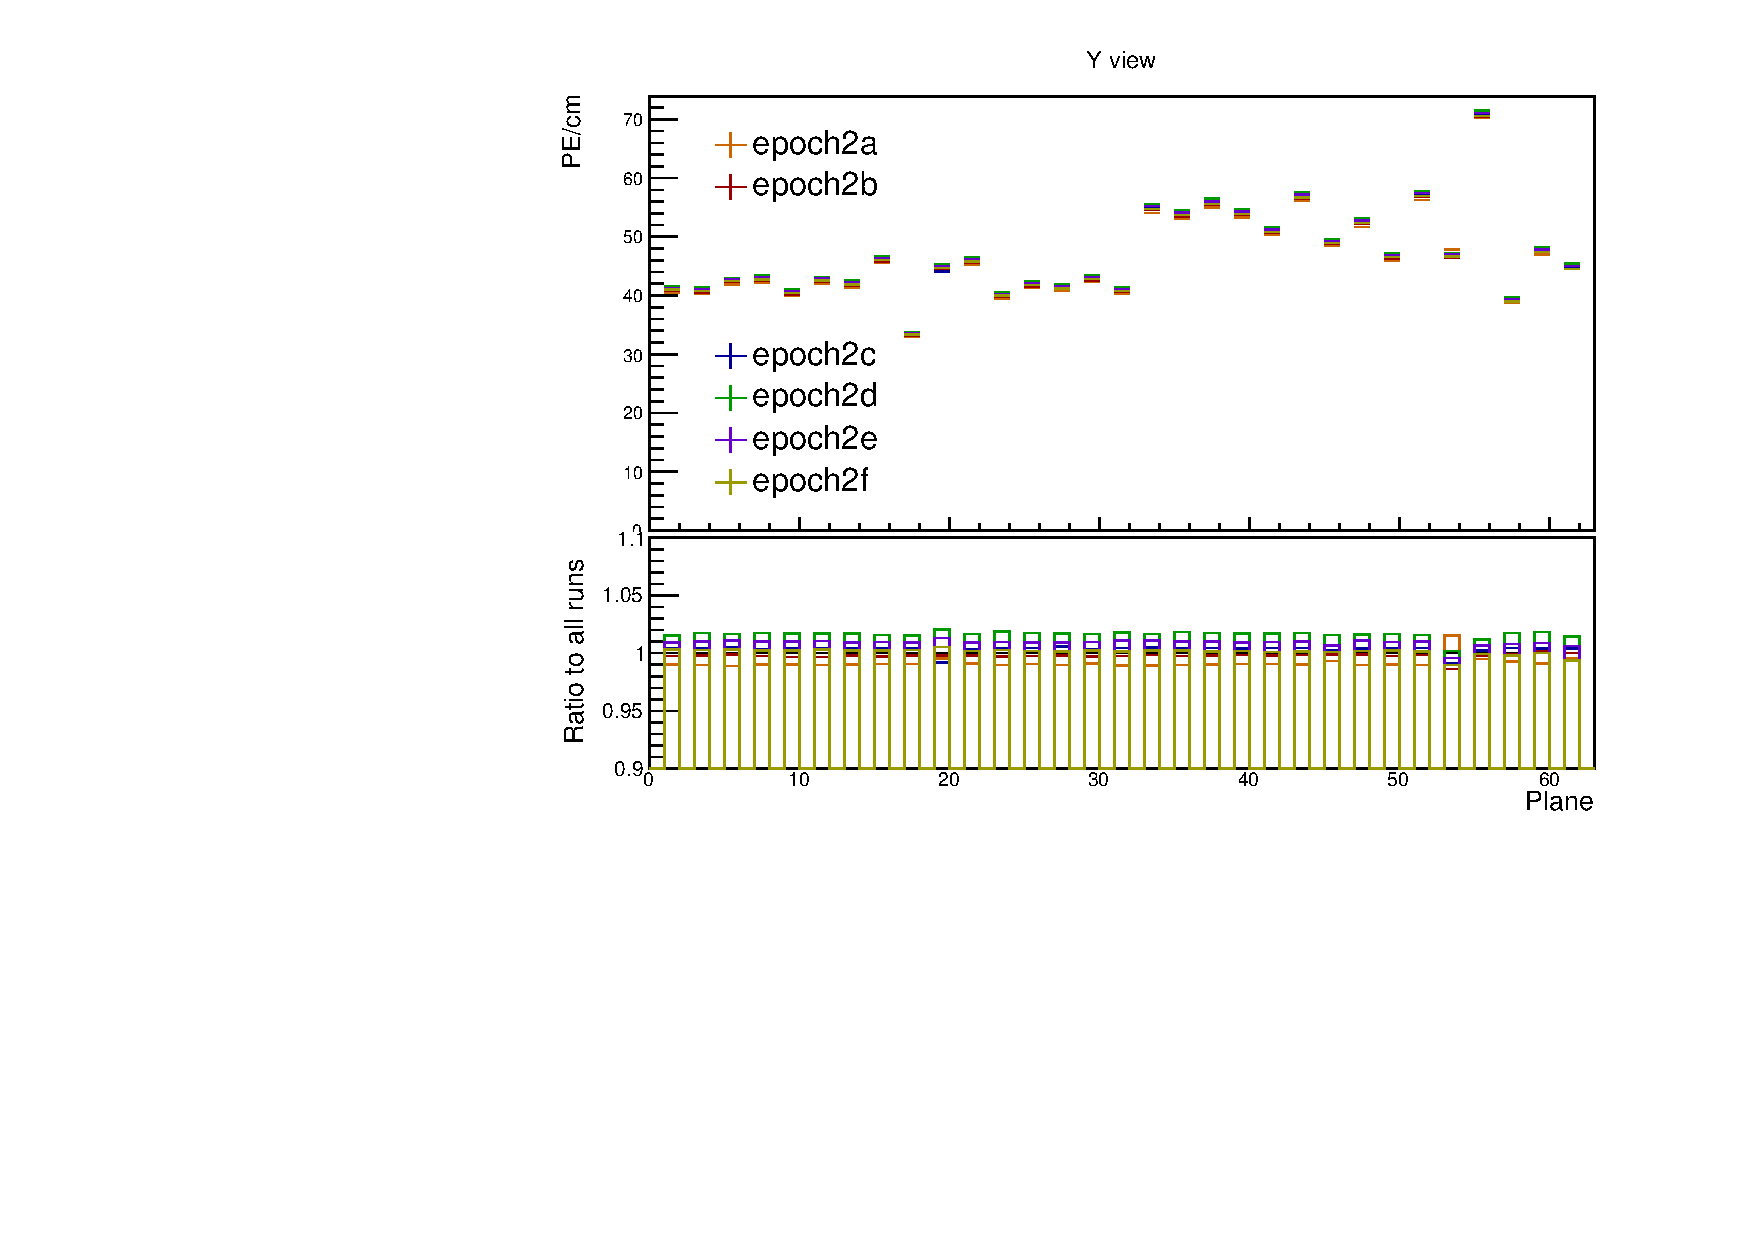
\includegraphics[width=\textwidth]{Plots/Attenprofs_P2Data_PlanePE_Y_Combined.pdf}
\end{subfigure}
\caption{Uncorrected average energy response as a function of planes for epochs in period 2.}
\label{figCalibhistPlanePE_period2}
\end{figure}

\subsubsection*{Period 2 relative calibration results}

The results of the attenuation fit for period 2 are summarised on Fig. \ref{figCellCentreResponsePeriod2}, showing the fitted response at the centre of each cell, or a blank cell if it failed calibration.

\begin{figure}[h]
\centering
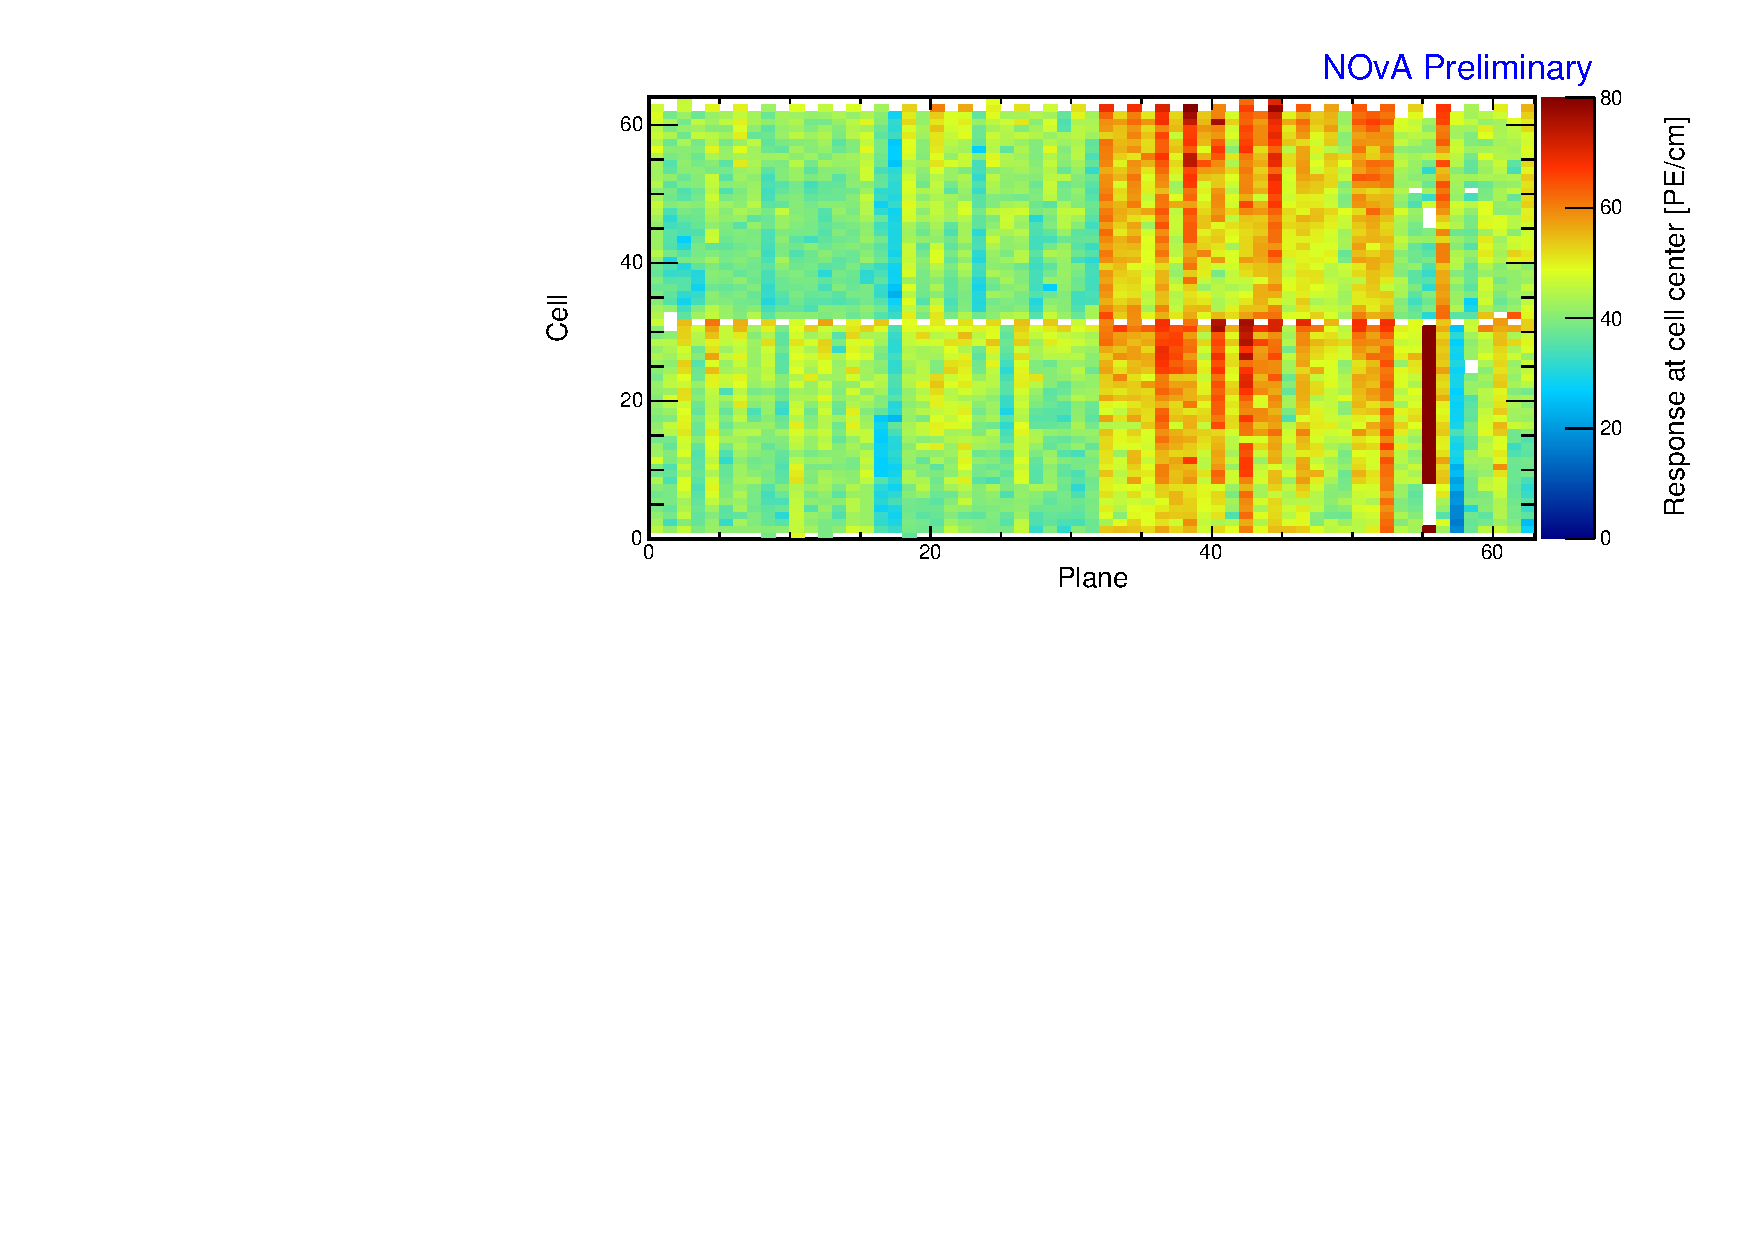
\includegraphics[width=0.9\textwidth]{Plots/CellResponseAtCentre_period2_Limited_NOvAPlotStyle.pdf}
\caption{Overview of the relative calibration results for the Test Beam detector period 2 data. Each cell represents the result of the attenuation fit to the energy response in the centre of that cell. The blank cells are uncalibrated.}
\label{figCellCentreResponsePeriod2}
\end{figure}

Most of the cells have an expected response, with steady rise towards the readout and a drop on the edges, as shown on the left plot of Fig. \ref{figAttenfitResultsPerio2_ZippedFibers}.

Some cells have a non-flat response across the cell, with one or more regions with a drop in the energy response, as shown on the right plot of Fig. \ref{figAttenfitResultsPerio2_ZippedFibers}. These low regions are (almost certainly) a real physical effect caused by zipped, or possibly even twisted fibres \cite{NOVA-doc-43249}, present in all of NOvA's detectors. Relative calibration corrects for this effect in data, but zipped fibres are not included in simulation, for any of the detectors. This could potentially cause issues with the ADC threshold in simulation.

\begin{figure}[h]
  \begin{subfigure}{0.5\textwidth}
    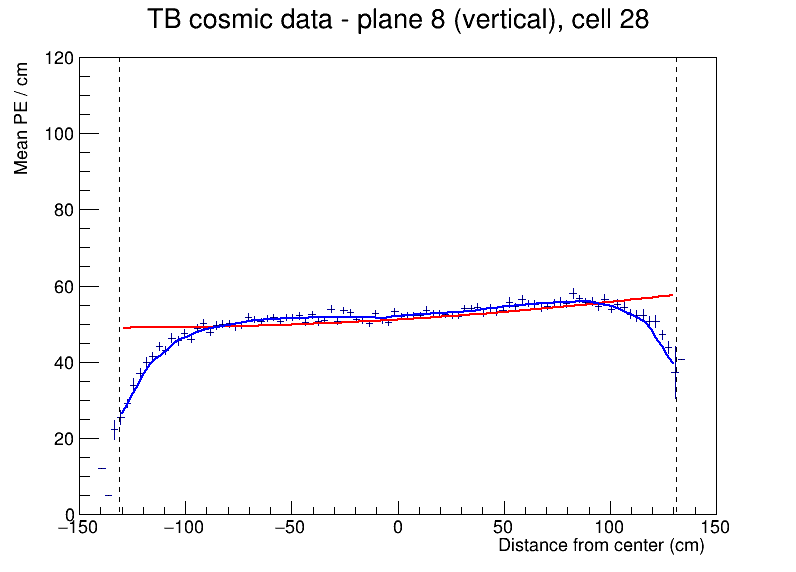
\includegraphics[width=\linewidth]{RelativeCalibrationResults/p2_008_028.png}
  \end{subfigure}
  \begin{subfigure}{0.5\textwidth}
    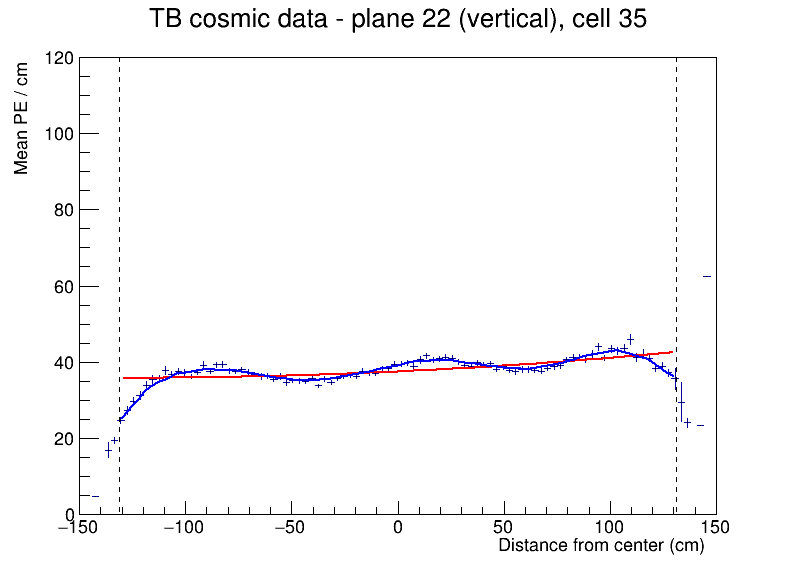
\includegraphics[width=\linewidth]{RelativeCalibrationResults/p2_022_035.png}
  \end{subfigure}
  \caption{Attenuation fits for a selection of cells in period 2. Left plot shows an example of the standard energy deposition in the Test Beam. Right plot shows the effect of zipped fibres.}
  \label{figAttenfitResultsPerio2_ZippedFibers}
\end{figure}

Since the underfilled cells were marked as bad channels we didn't attempt to calibrate them. Their neighbours have fewer events due to the tricell condition, but majority of them pass the calibration condition, as shown on Fig. \ref{figAttenfitResultsPerio2_UnderfilledCells}. The neighbouring cells in plane 1 don't pass calibration due to low statistics and therefore large fluctuations, as shown on Fig. \ref{figAttenfitResultsPerio2_UnderfilledCellsPlane01}. This is likely due to a combination of the tricell condition and plane 1 being on the edge of the detector, which typically has fewer (accepted) hits than the center, as shown on Fig. \ref{figCalibhist_period2}.

\begin{figure}[h]
  \begin{subfigure}{0.5\textwidth}
    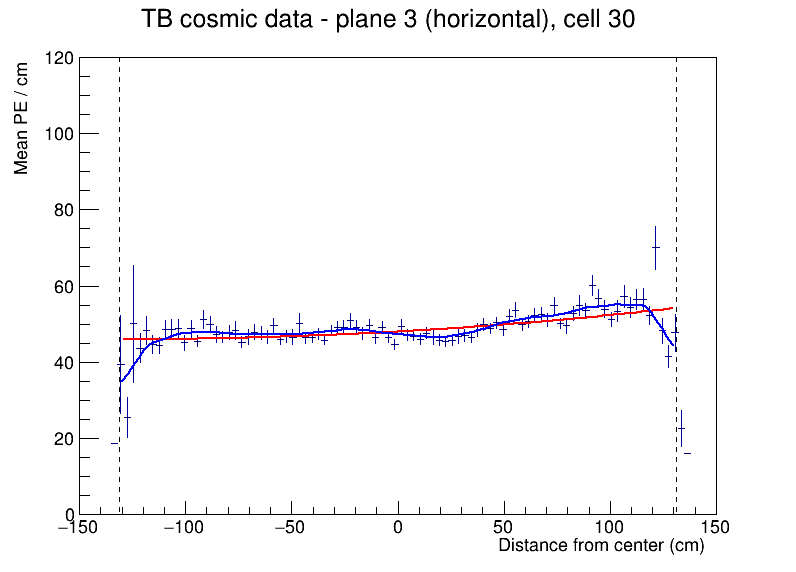
\includegraphics[width=\linewidth]{RelativeCalibrationResults/p2_003_030.png}
  \end{subfigure}
  \begin{subfigure}{0.5\textwidth}
    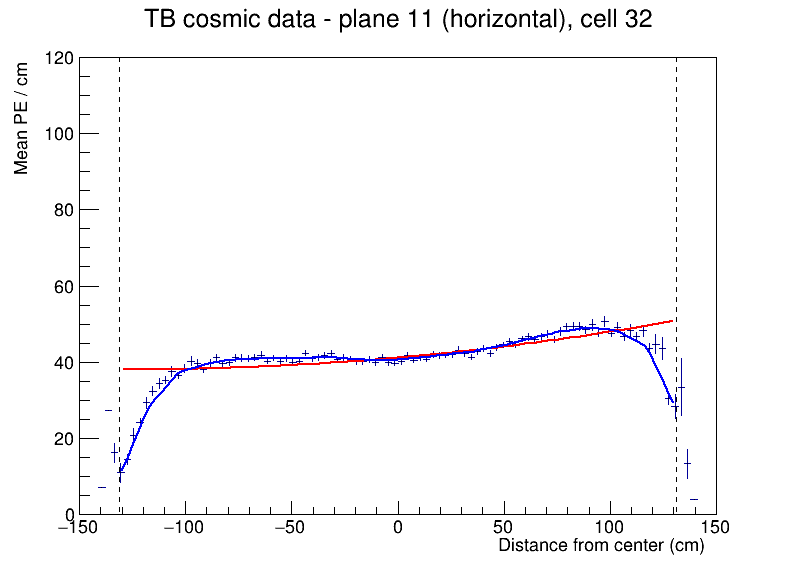
\includegraphics[width=\linewidth]{RelativeCalibrationResults/p2_011_032.png}
  \end{subfigure}
  \caption{Fit to the energy response in period 2. The cells neighbouring the underfilled cells have fewer events and therefore larger fluctuations than the "usual" Test Beam cell.}
  \label{figAttenfitResultsPerio2_UnderfilledCells}
\end{figure}

\begin{figure}[h]
  \begin{subfigure}{0.5\textwidth}
    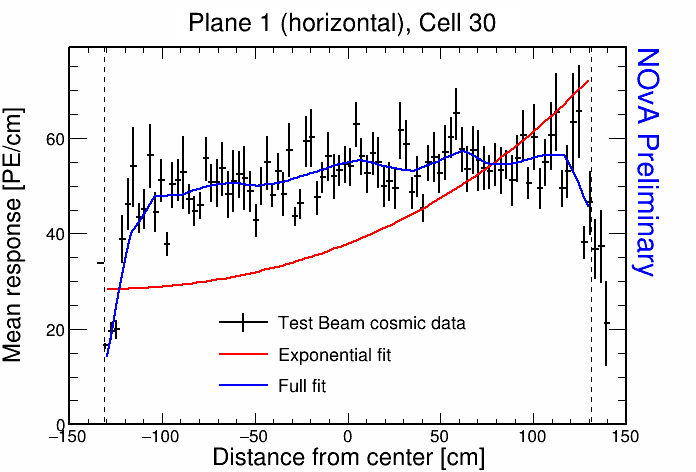
\includegraphics[width=\linewidth]{RelativeCalibrationResults/p2_001_030.png}
  \end{subfigure}
  \begin{subfigure}{0.5\textwidth}
    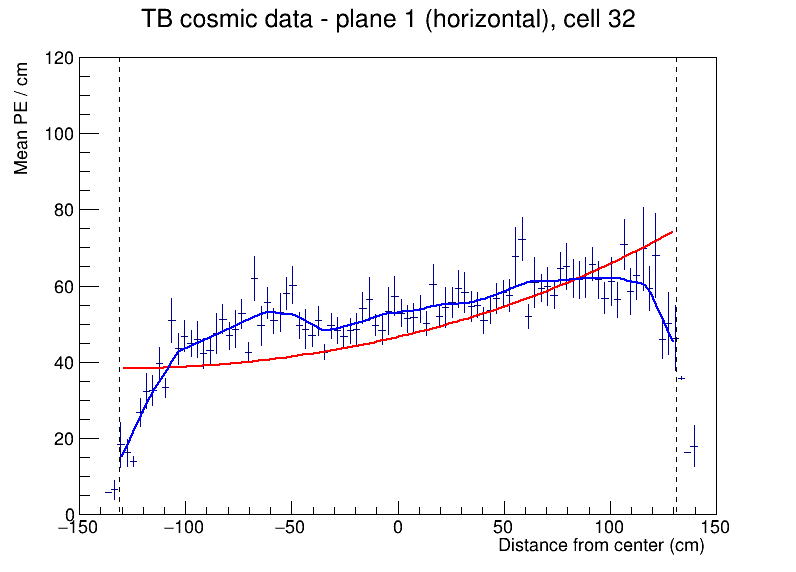
\includegraphics[width=\linewidth]{RelativeCalibrationResults/p2_001_032.png}
  \end{subfigure}
  \caption{Fit to the energy response in period 2. The neighbouring cells to the underfilled cells in plane 1 are uncalibrated due to low statistics.}
  \label{figAttenfitResultsPerio2_UnderfilledCellsPlane01}
\end{figure}

The left half of plane 55 has more than $3\times$ larger response than it's surrounding planes, as shown on the left plot of Fig. \ref{figAttenfitResultsPerio2_FaultyFEB}. Similarly, the left half of plane 57 has slightly lower response than the surrounding planes, as shown on the right plot of Fig. \ref{figAttenfitResultsPerio2_FaultyFEB}. This is due to the corresponding APDs/FEBs incorrectly recording different energy response than the real energy deposited in the detector. Since this effect is present for all data, not only for the cosmic muons used for calibration, it is important to correctly calibrate it out. The issue can arise if these FEBs have been "faulty" only for a limited time of the entire calibrated period. Since we are doing the attenuation fit on the average response across the whole calibrated period, if an FEB records a standard response for half of the time and $7\times$ larger response for the seconds half, calibration is going to assume the response was $4\times$ larger the entire time, which is incorrect. Since both of these planes are in the back of the detector, we decided to ignore this effect for period 2.

\begin{figure}[h]
  \begin{subfigure}{0.5\textwidth}
    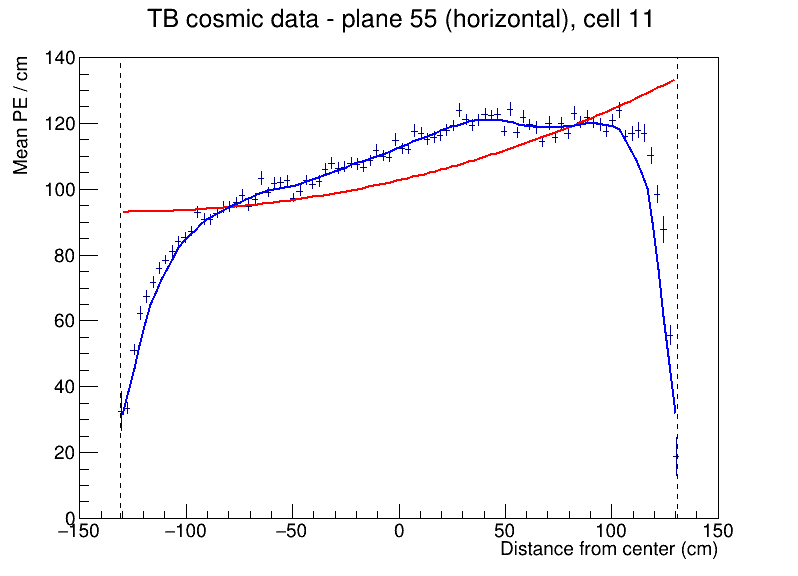
\includegraphics[width=\linewidth]{RelativeCalibrationResults/p2_055_011_extendedRange.png}
  \end{subfigure}
  \begin{subfigure}{0.5\textwidth}
    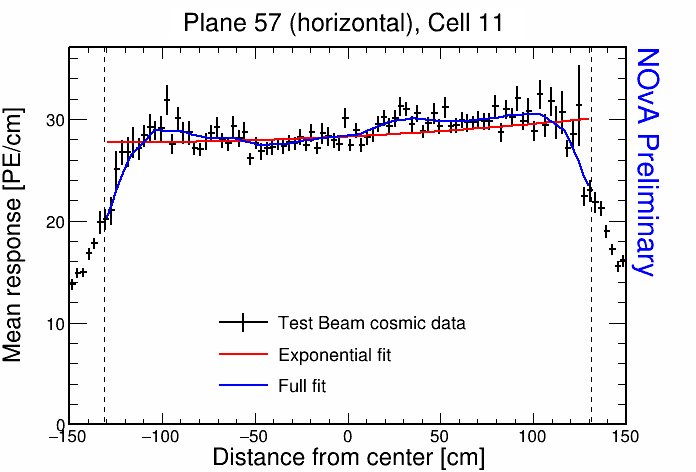
\includegraphics[width=\linewidth]{RelativeCalibrationResults/p2_057_011.png}
  \end{subfigure}
  \caption{Fit to the energy response in period 2. Lower halves of planes 55 and 57 have a different scale of energy response than the surrounding planes.}
  \label{figAttenfitResultsPerio2_FaultyFEB}
\end{figure}

The cells with (probably) swapped cables in plane 55 have almost no events, which affects both them and their neighbours as shown of Fig. \ref{figAttenfitResultsPerio2_SwappedCables}.

\begin{figure}[h]
  \begin{subfigure}{0.5\textwidth}
    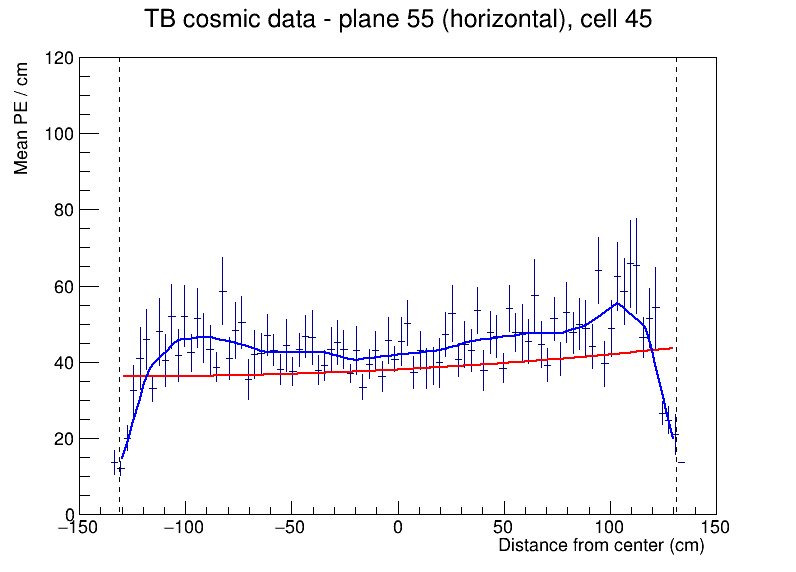
\includegraphics[width=\linewidth]{RelativeCalibrationResults/p2_055_045.png}
  \end{subfigure}
  \begin{subfigure}{0.5\textwidth}
    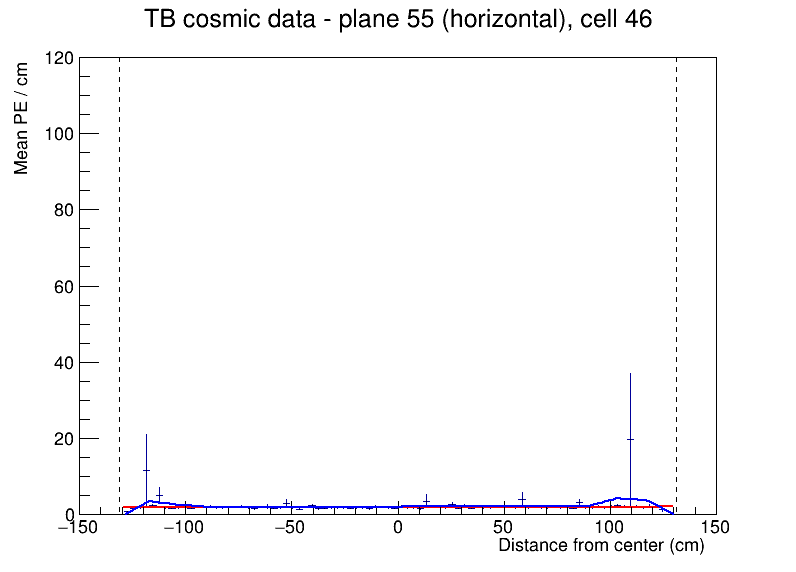
\includegraphics[width=\linewidth]{RelativeCalibrationResults/p2_055_046.png}
  \end{subfigure}
  \caption{Fit to the energy response in period 2. Cells with swapped readout cables have almost no recorded events as shown on the right plot. This also affect their neighbouring cells due to the tricell condition as shown on the left plot.}
  \label{figAttenfitResultsPerio2_SwappedCables}
\end{figure}

Several cells in the end of the Test Beam detector are uncalibrated due to the histogram bins on the edges of the cell having an unusually high response, or no events at all, as shown on Fig. \ref{figAttenfitResultsPerio2_CellEdge}. It is unknown if this is a real physical effect, possibly related to the fibres, or if it is unfiltered noise hits, or something else entirely. Since these cells are in the end of the detector, it is fairly safe to ignore them.

\begin{figure}[h]
  \begin{subfigure}{0.5\textwidth}
    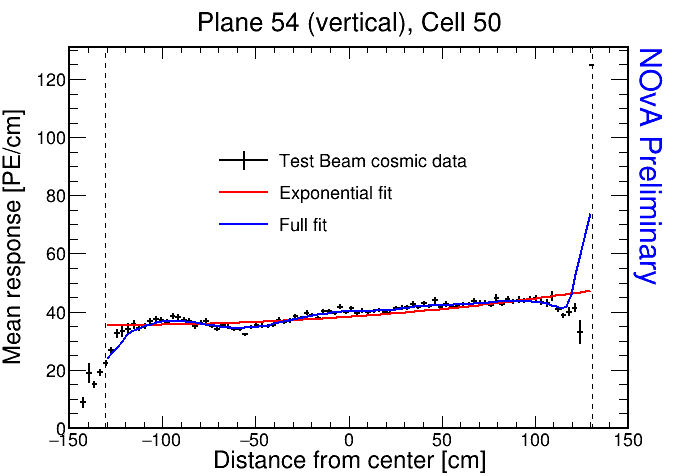
\includegraphics[width=\linewidth]{RelativeCalibrationResults/p2_054_050.png}
  \end{subfigure}
  \begin{subfigure}{0.5\textwidth}
    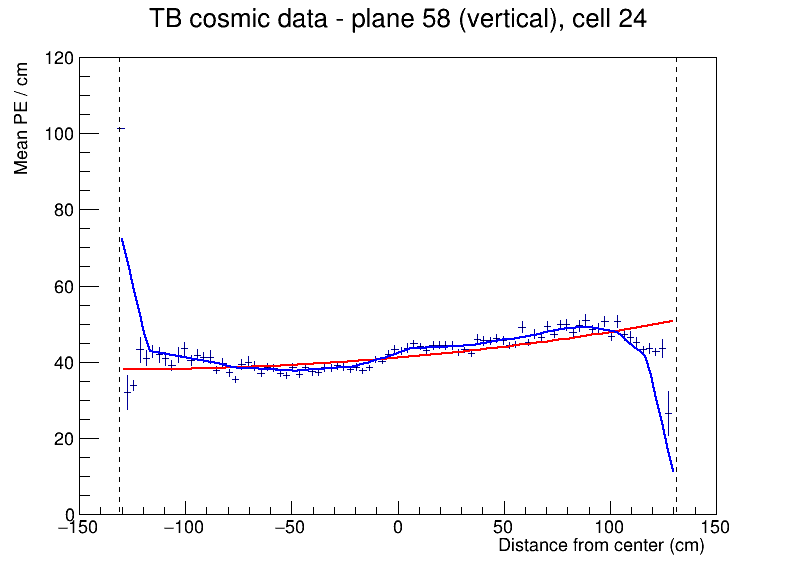
\includegraphics[width=\linewidth]{RelativeCalibrationResults/p2_058_024.png}
  \end{subfigure}
  \begin{subfigure}{0.5\textwidth}
    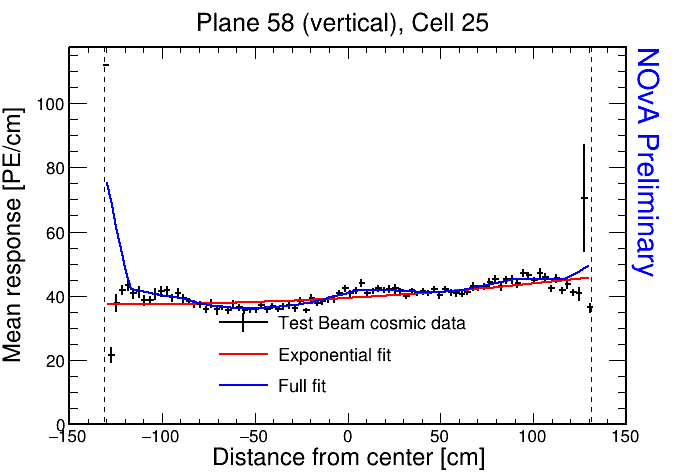
\includegraphics[width=\linewidth]{RelativeCalibrationResults/p2_058_025.png}
  \end{subfigure}
  \begin{subfigure}{0.5\textwidth}
    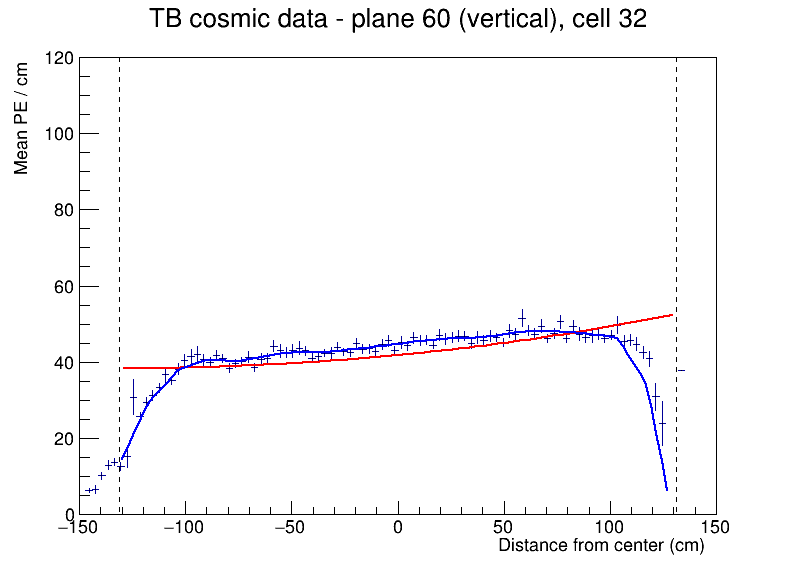
\includegraphics[width=\linewidth]{RelativeCalibrationResults/p2_060_032.png}
  \end{subfigure}
  \caption{Fit to the energy response in period 2. Examples of cells that have an unusually high or low energy response at the edge of the cell. These cells are not calibrated.}
  \label{figAttenfitResultsPerio2_CellEdge}
\end{figure}

\FloatBarrier
\subsection{Period 3 data}
The underfilled cells were refilled (or overfilled) during the period 3 data taking. This was the main motivation for dividing period 3 into individual epochs as shown on table \ref{tabTestBeamPeriod3Epochs}. One more major event that could impact the Test Beam data is the replacement of several faulty FEBs, which motivated the creation of epoch 3e.

\begin{table}[!ht]
\centering
\def\arraystretch{1.4}
\begin{tabular}{m{0.11\textwidth} m{0.22\textwidth} m{0.55\textwidth}}
Name & Start date & Reason for creating the epoch\\\hline
Epoch 3a & January $12^{\textsf{th}}$ 2021 & Underfilled cells\\
Epoch 3b & April $21^{\textsf{st}}$ 2021 & Overfilling the back 9 horizontal planes and the 7th horizontal plane from the front\\
Epoch 3c & April $27^{\textsf{th}}$ 2021 & Overfilling of the 15 front horizontal planes (except the 7th, which was already done) and the 14th horizontal plane\\
Epoch 3d & April $30^{\textsf{th}}$ 2021 & Overfilling of the remaining 8 horizontal planes\\
Epoch 3e & May $12^{\textsf{th}}$ 2021 & FEB swaps
\end{tabular}
\caption{Test Beam period 3 epochs, their start dates and the reason for their separation.}
\label{tabTestBeamPeriod3Epochs}
\end{table}

The refilling of the underfilled cells can be clearly seen on the cell hits distribution on Fig. \ref{figCalibhist_period3} and on the distribution of energy deposition across horizontal cells (Y view) on Fig. \ref{figCalibhistCellPE_period3}.

\begin{figure}[!hbtp]
\centering
\begin{subfigure}[b]{\textwidth}
\centering
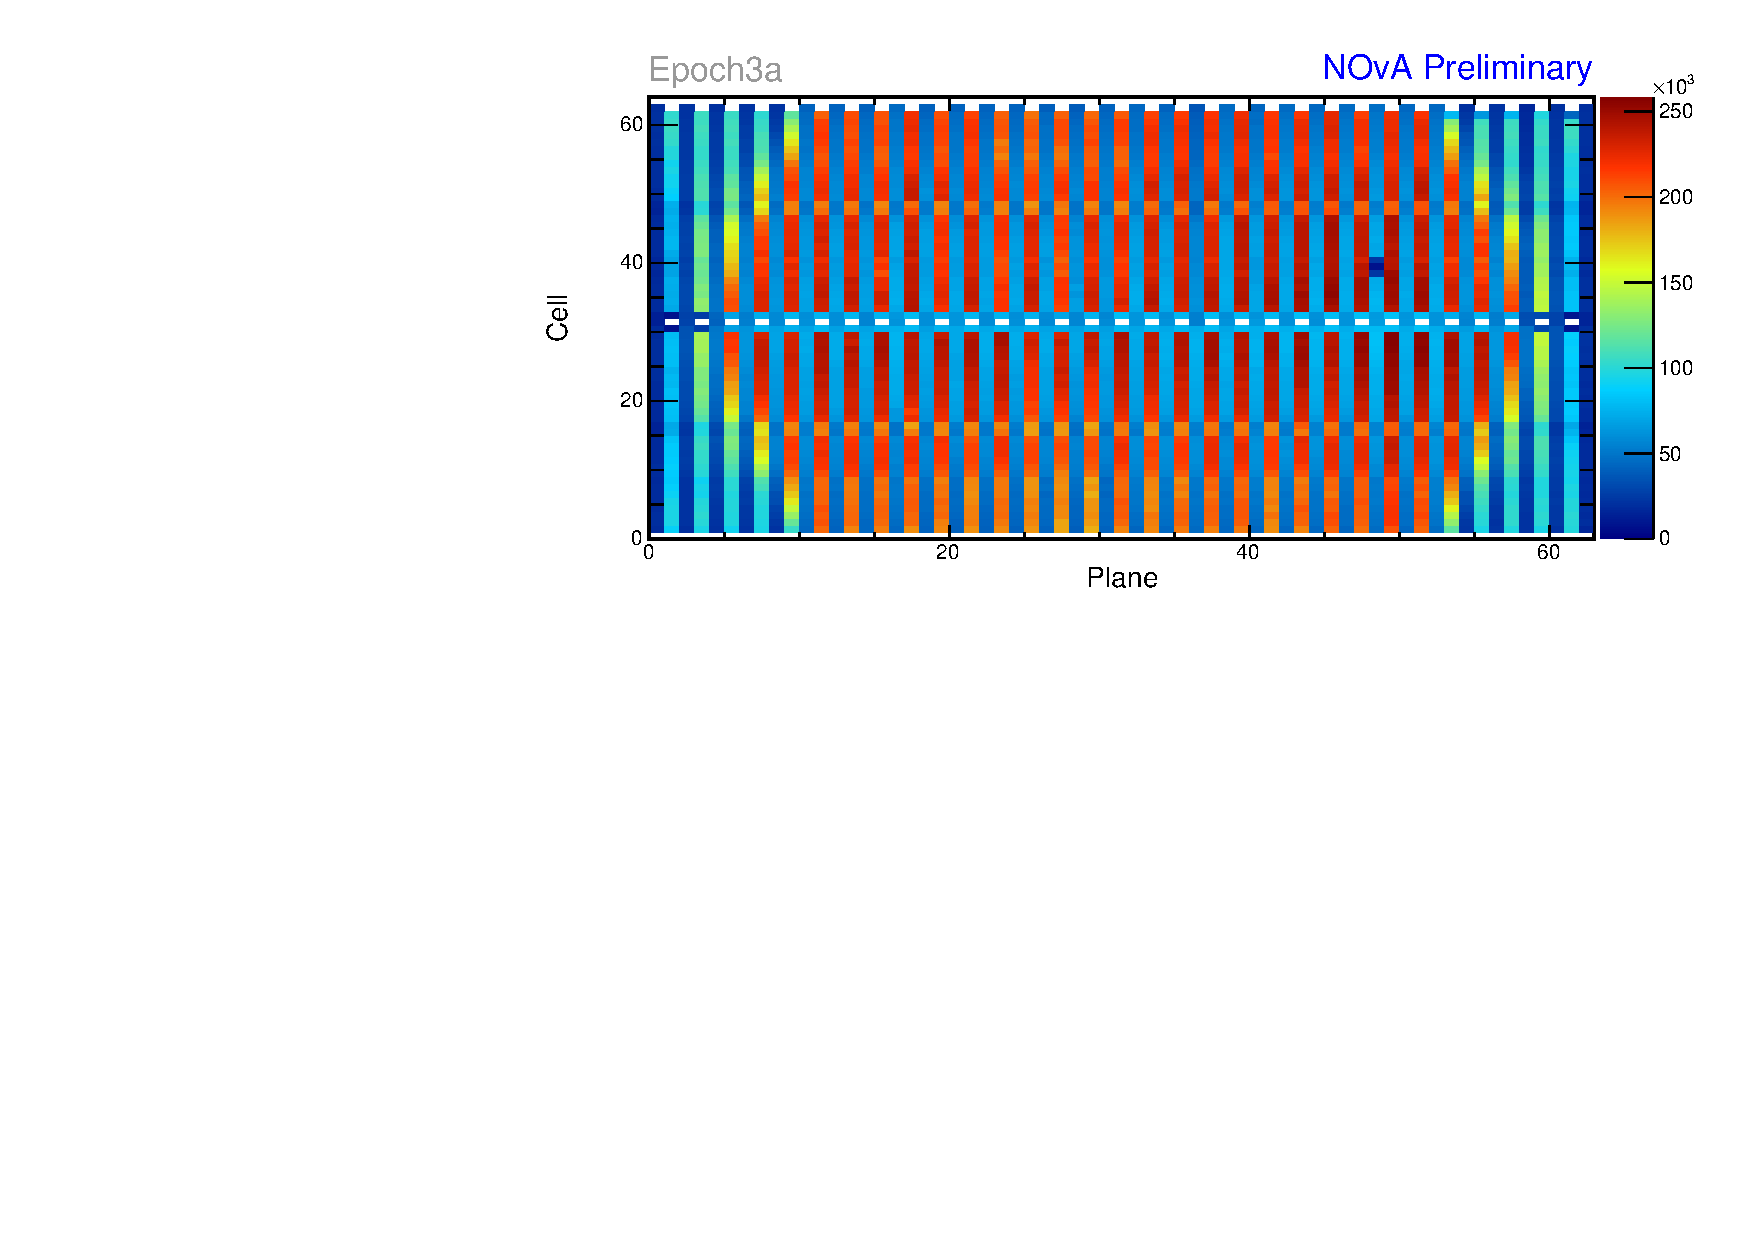
\includegraphics[width=0.9\textwidth]{Plots/Attenprofs_P3Data_CellPlane_Epoch3a.pdf}
\end{subfigure}
\begin{subfigure}[b]{\textwidth}
\centering
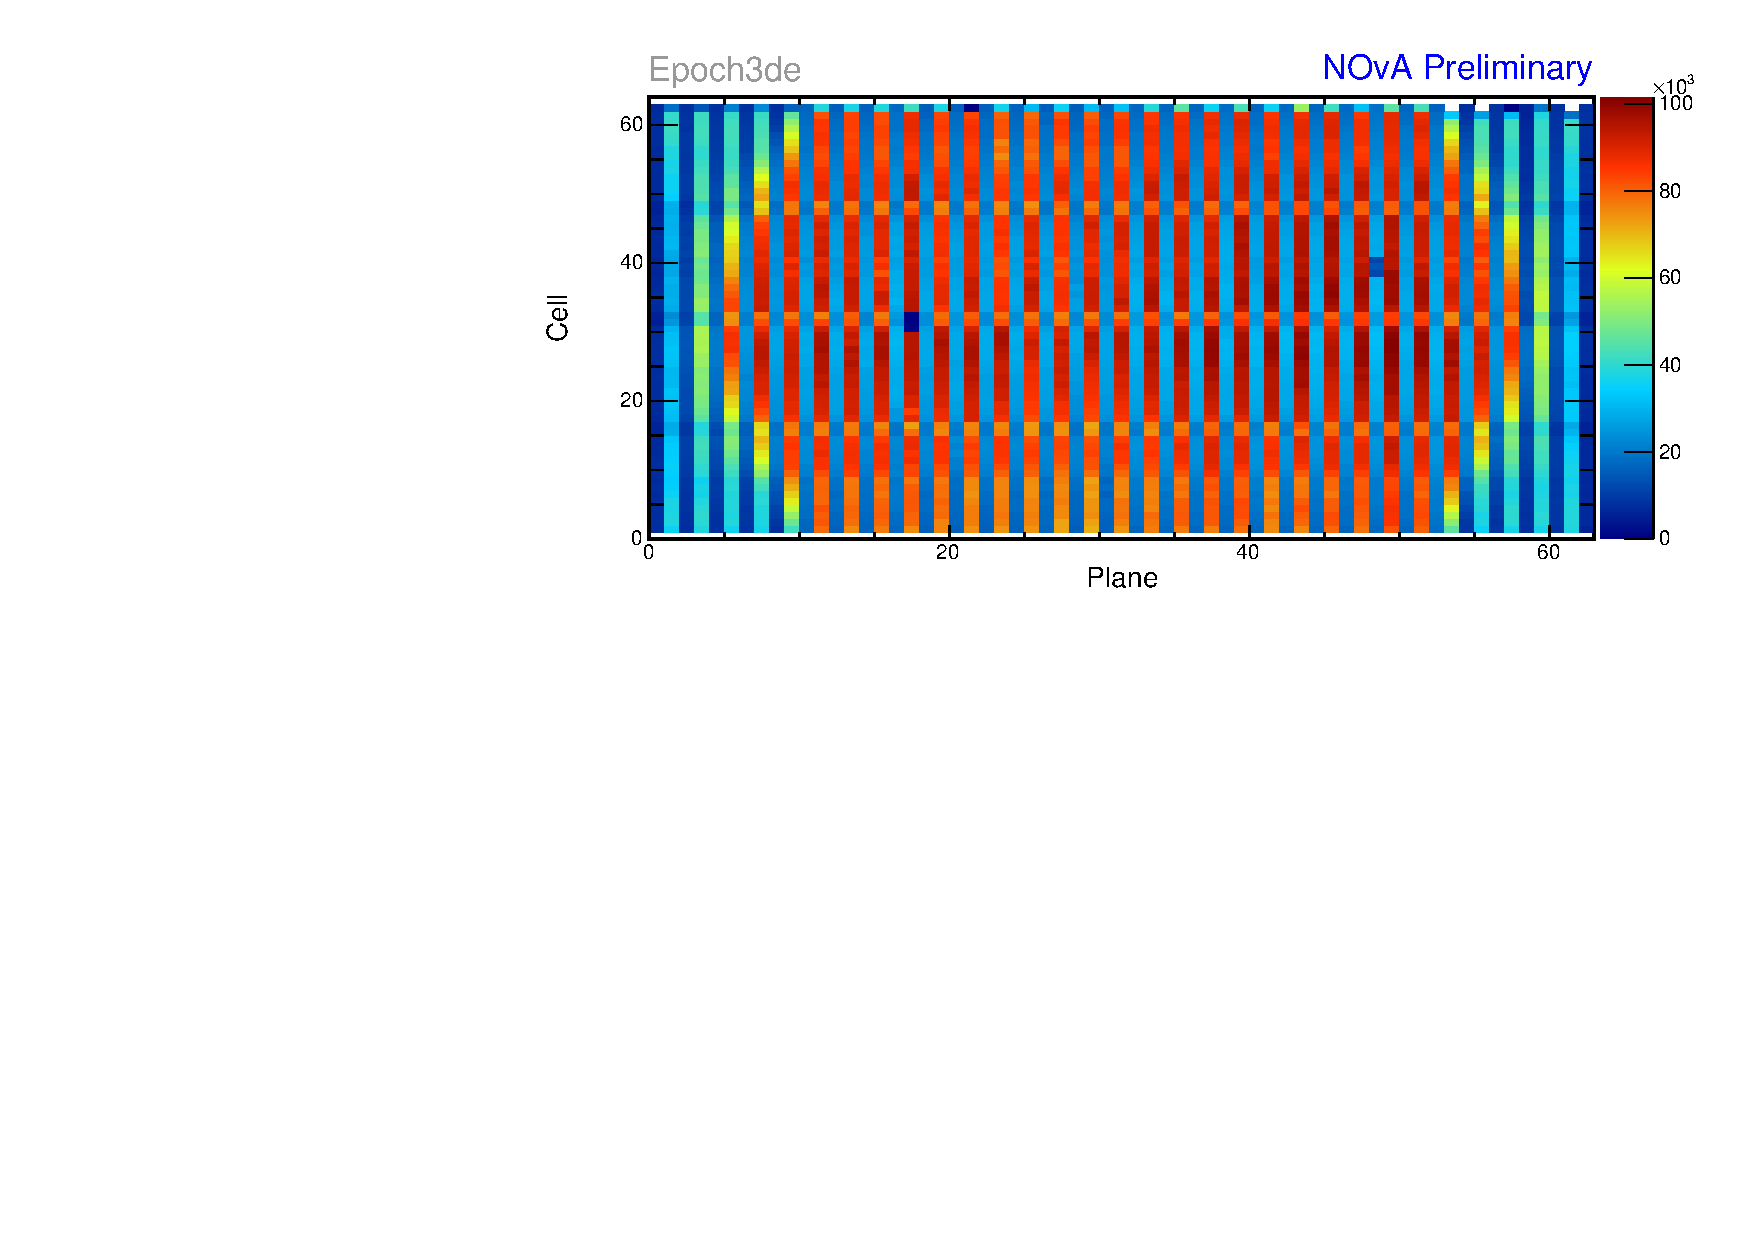
\includegraphics[width=0.9\textwidth]{Plots/Attenprofs_P3Data_CellPlane_Epoch3de.pdf}
\end{subfigure}
\caption{Distribution of events in the period 3 Test Beam data calibration sample. Comparison of Epoch 3a data before the refilling of the underfilled cells and Epoch 3de (combination of Epochs 3d and 3e) after the full refilling.}
\label{figCalibhist_period3}
\end{figure}

From the cell hits distributions we can also see there are a few channels (cells) that were likely dead for a certain time and weren't recording the same number of events as the surrounding cells. This is specifically plane 48, cell 39 in all of period 3 and plane 18, cell 31 in epochs 3d and 3e.

The energy distributions across cells and planes in the X view (vertical) on Fig. \ref{figCalibhistCellPE_period3} and \ref{figCalibhistPlanePE_period3} shows, that the top half of plane 58 has a very distinctly different energy deposition compared to the rest of the cells. However Fig. \ref{figCalibhist_period3} shows that this part has the same number of events. This is the FEB, that has the largest impact on the calibration (and overall) out of the faulty FEBs replaced before the start of epoch 3e.

\begin{figure}[!hbtp]
\centering
\begin{subfigure}[b]{0.495\textwidth}
\centering
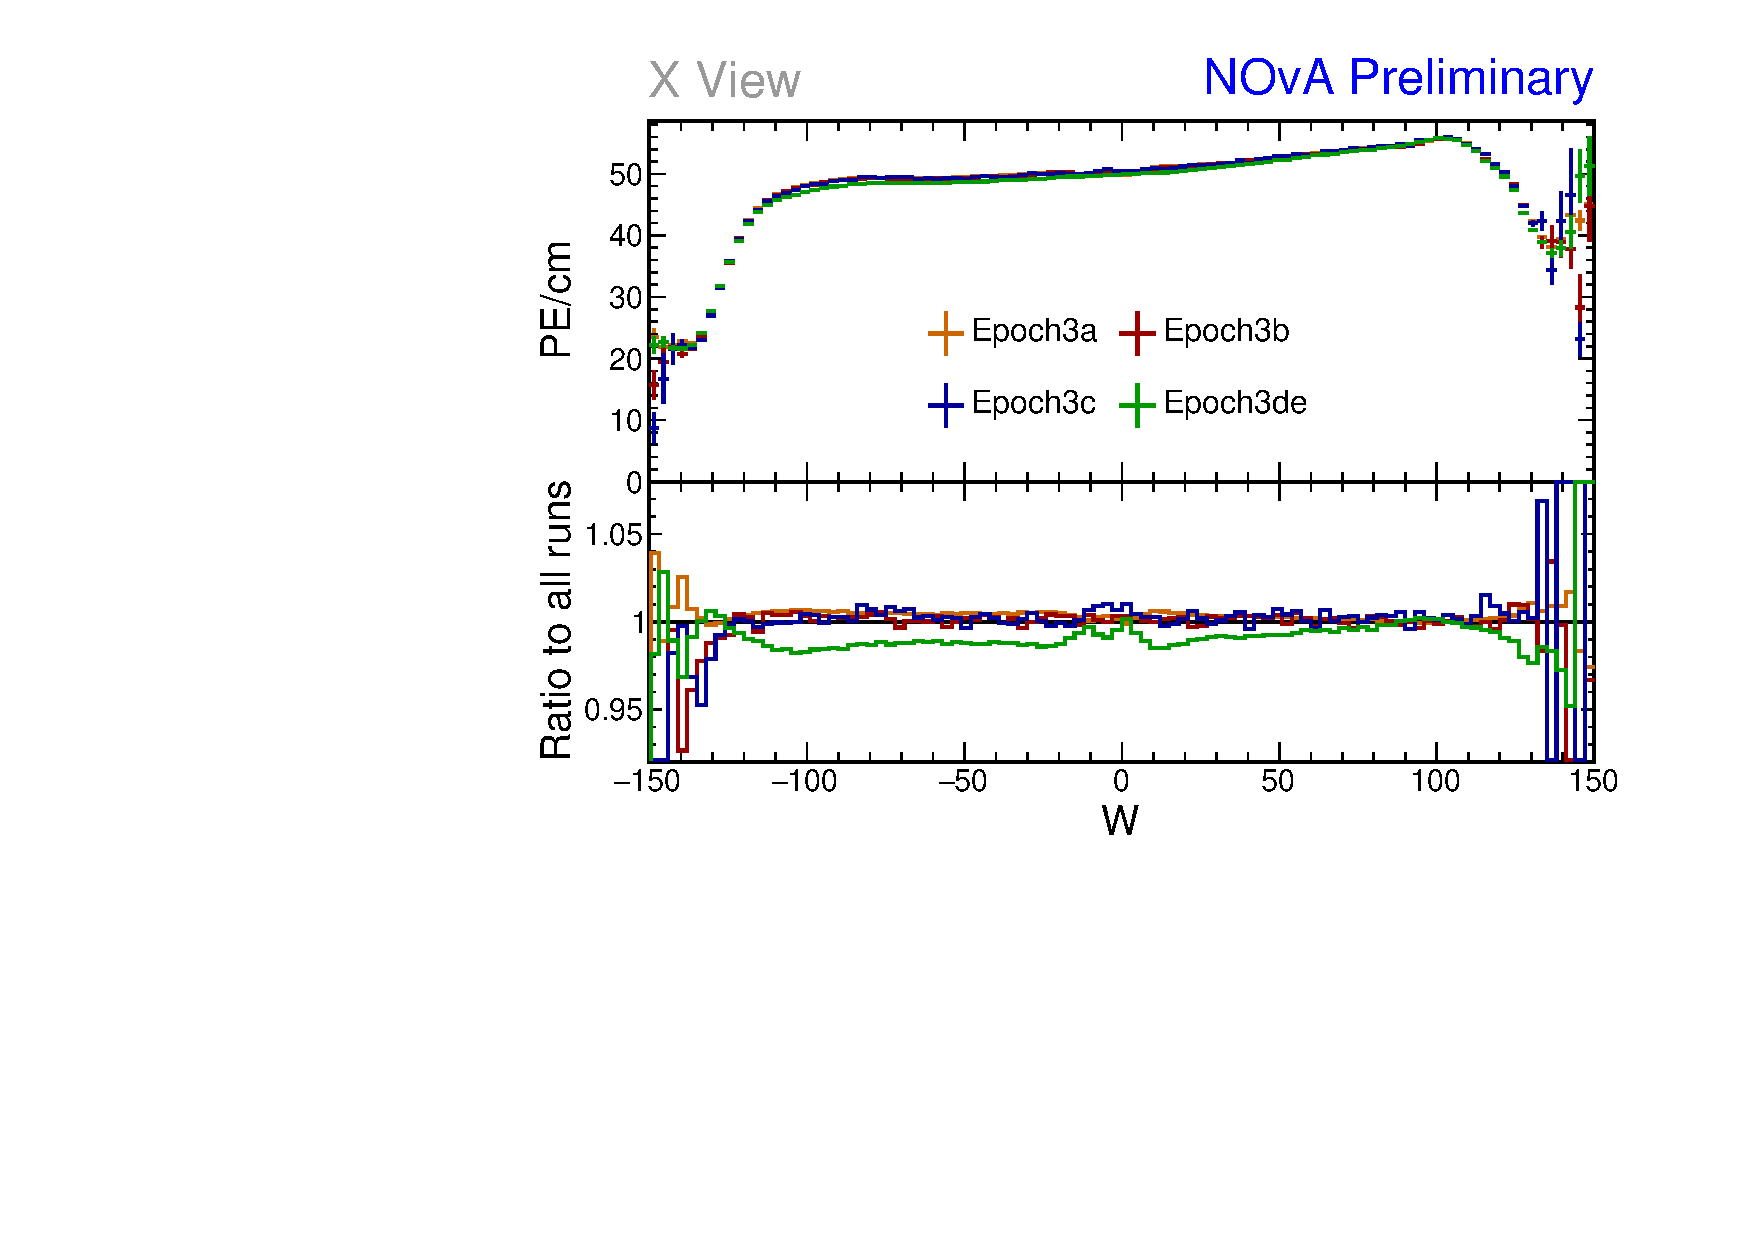
\includegraphics[width=\textwidth]{Plots/Attenprofs_P3Data_WPE_corr_xy_X_Combined.pdf}
\end{subfigure}
\begin{subfigure}[b]{0.495\textwidth}
\centering
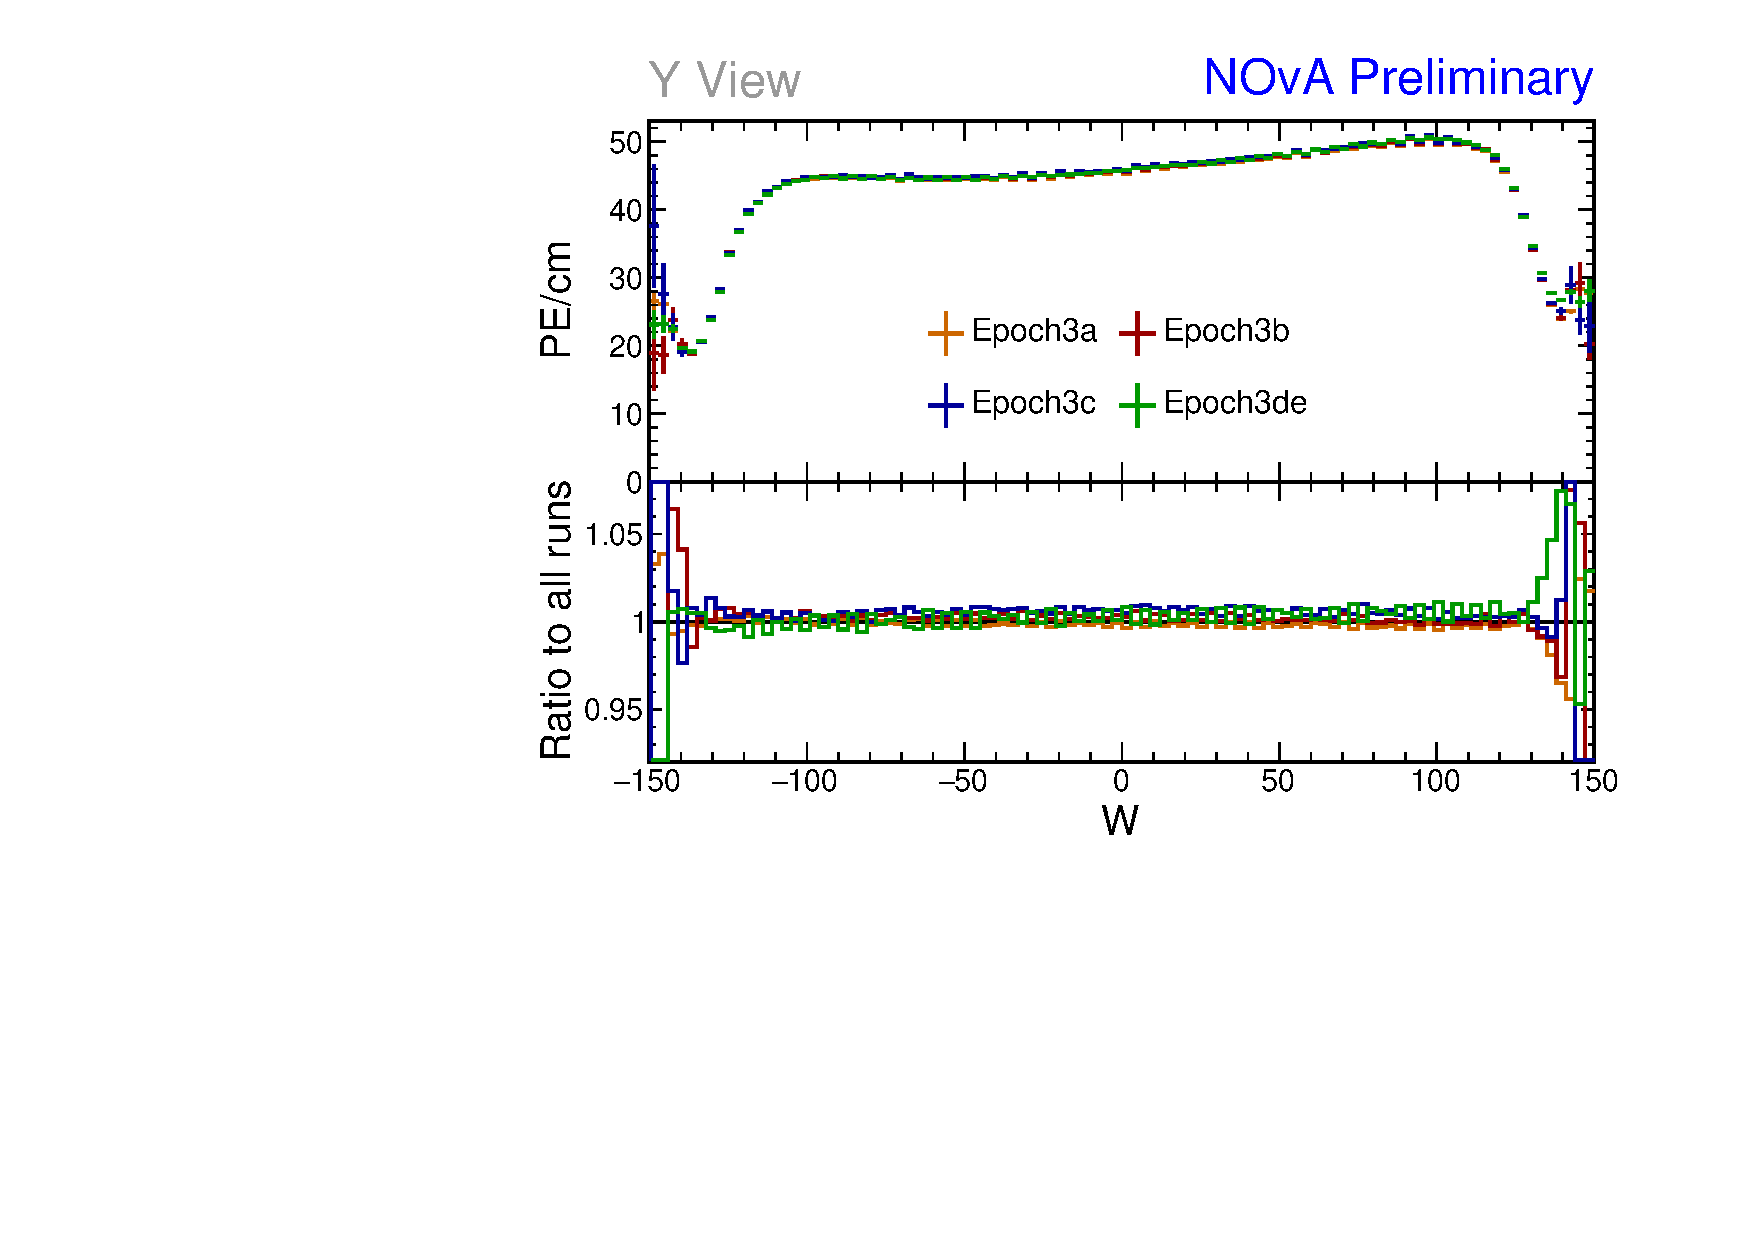
\includegraphics[width=\textwidth]{Plots/Attenprofs_P3Data_WPE_corr_xy_Y_Combined.pdf}
\end{subfigure}
\caption{Uncorrected average energy response as a function of the position within a cell (w) for epochs in period 3.}
\label{figCalibhistWPE_period3}
\end{figure}

\begin{figure}[!hbtp]
\centering
\begin{subfigure}[b]{0.495\textwidth}
\centering
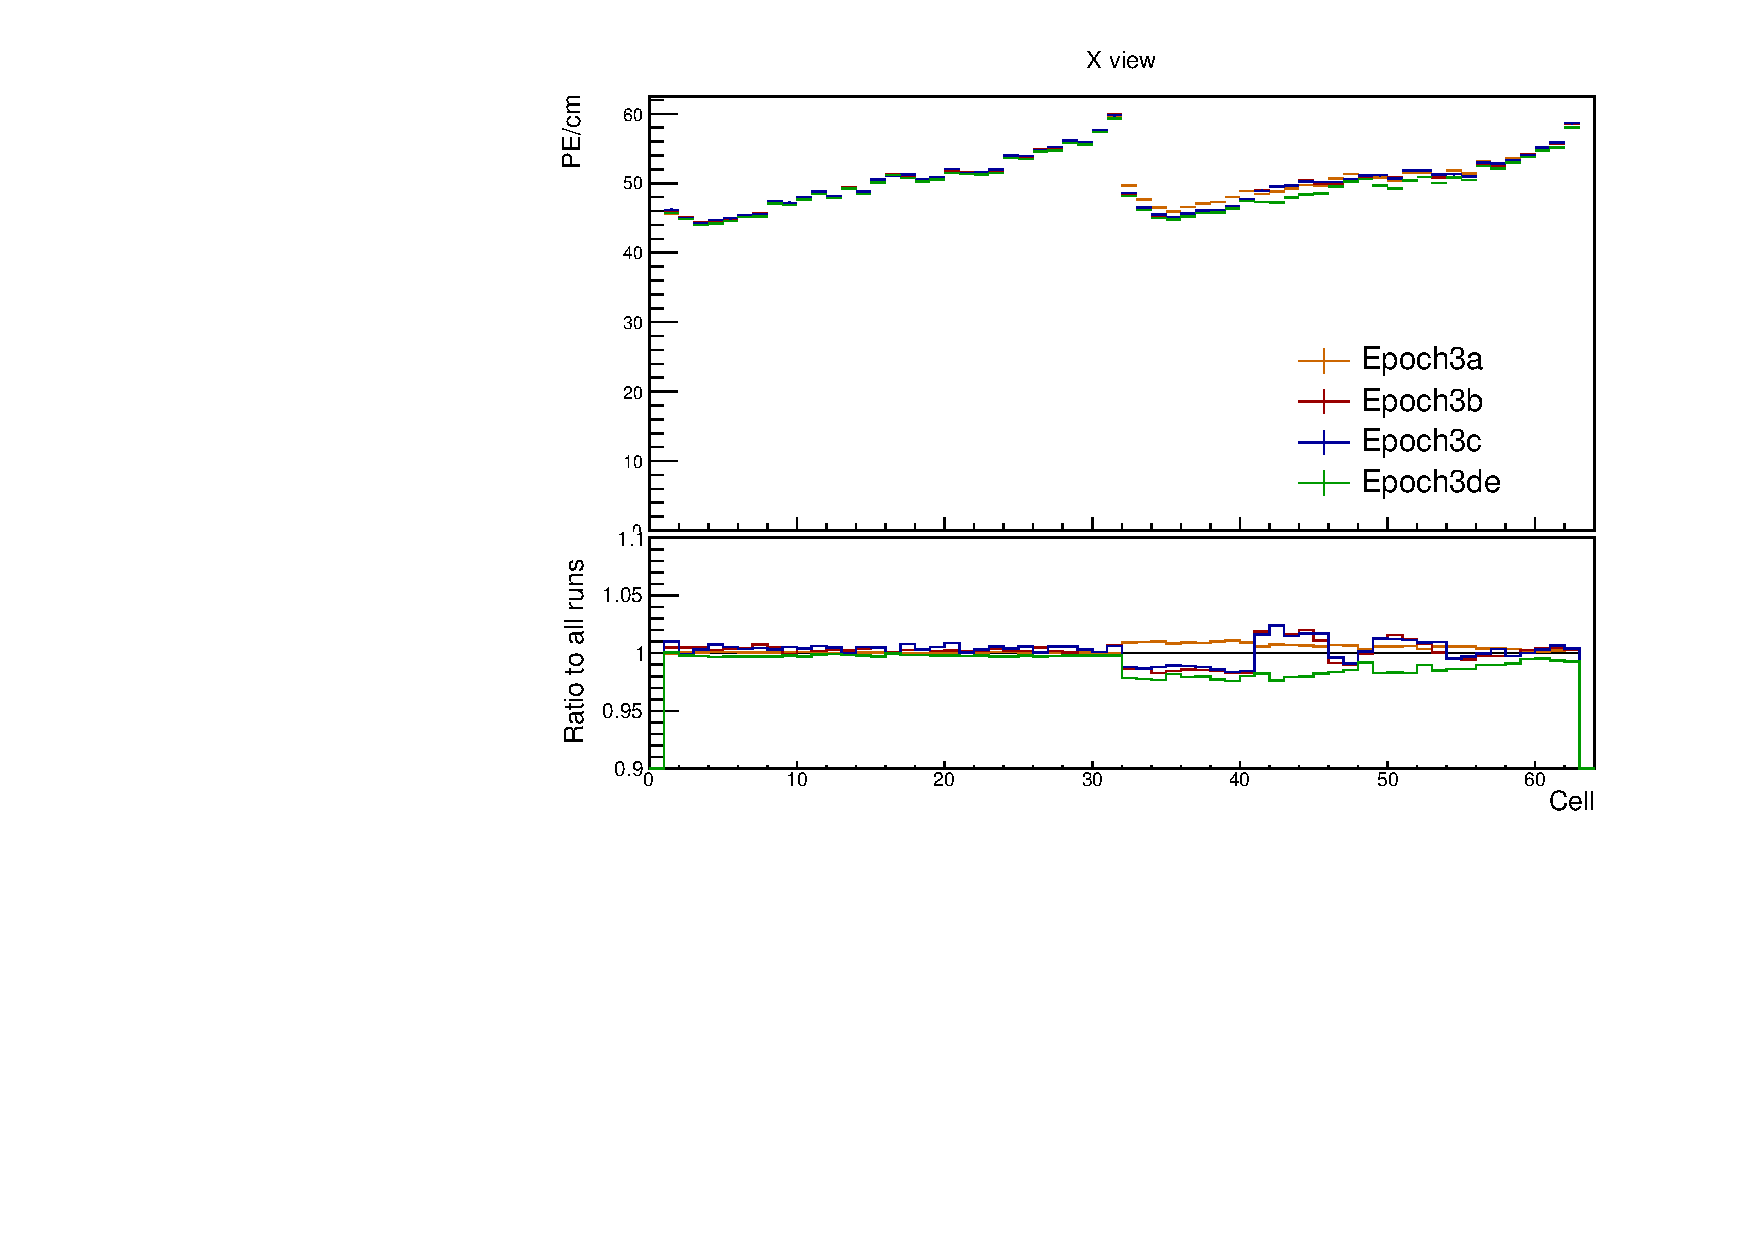
\includegraphics[width=\textwidth]{Plots/Attenprofs_P3Data_CellPE_X_Combined.pdf}
\end{subfigure}
\begin{subfigure}[b]{0.495\textwidth}
\centering
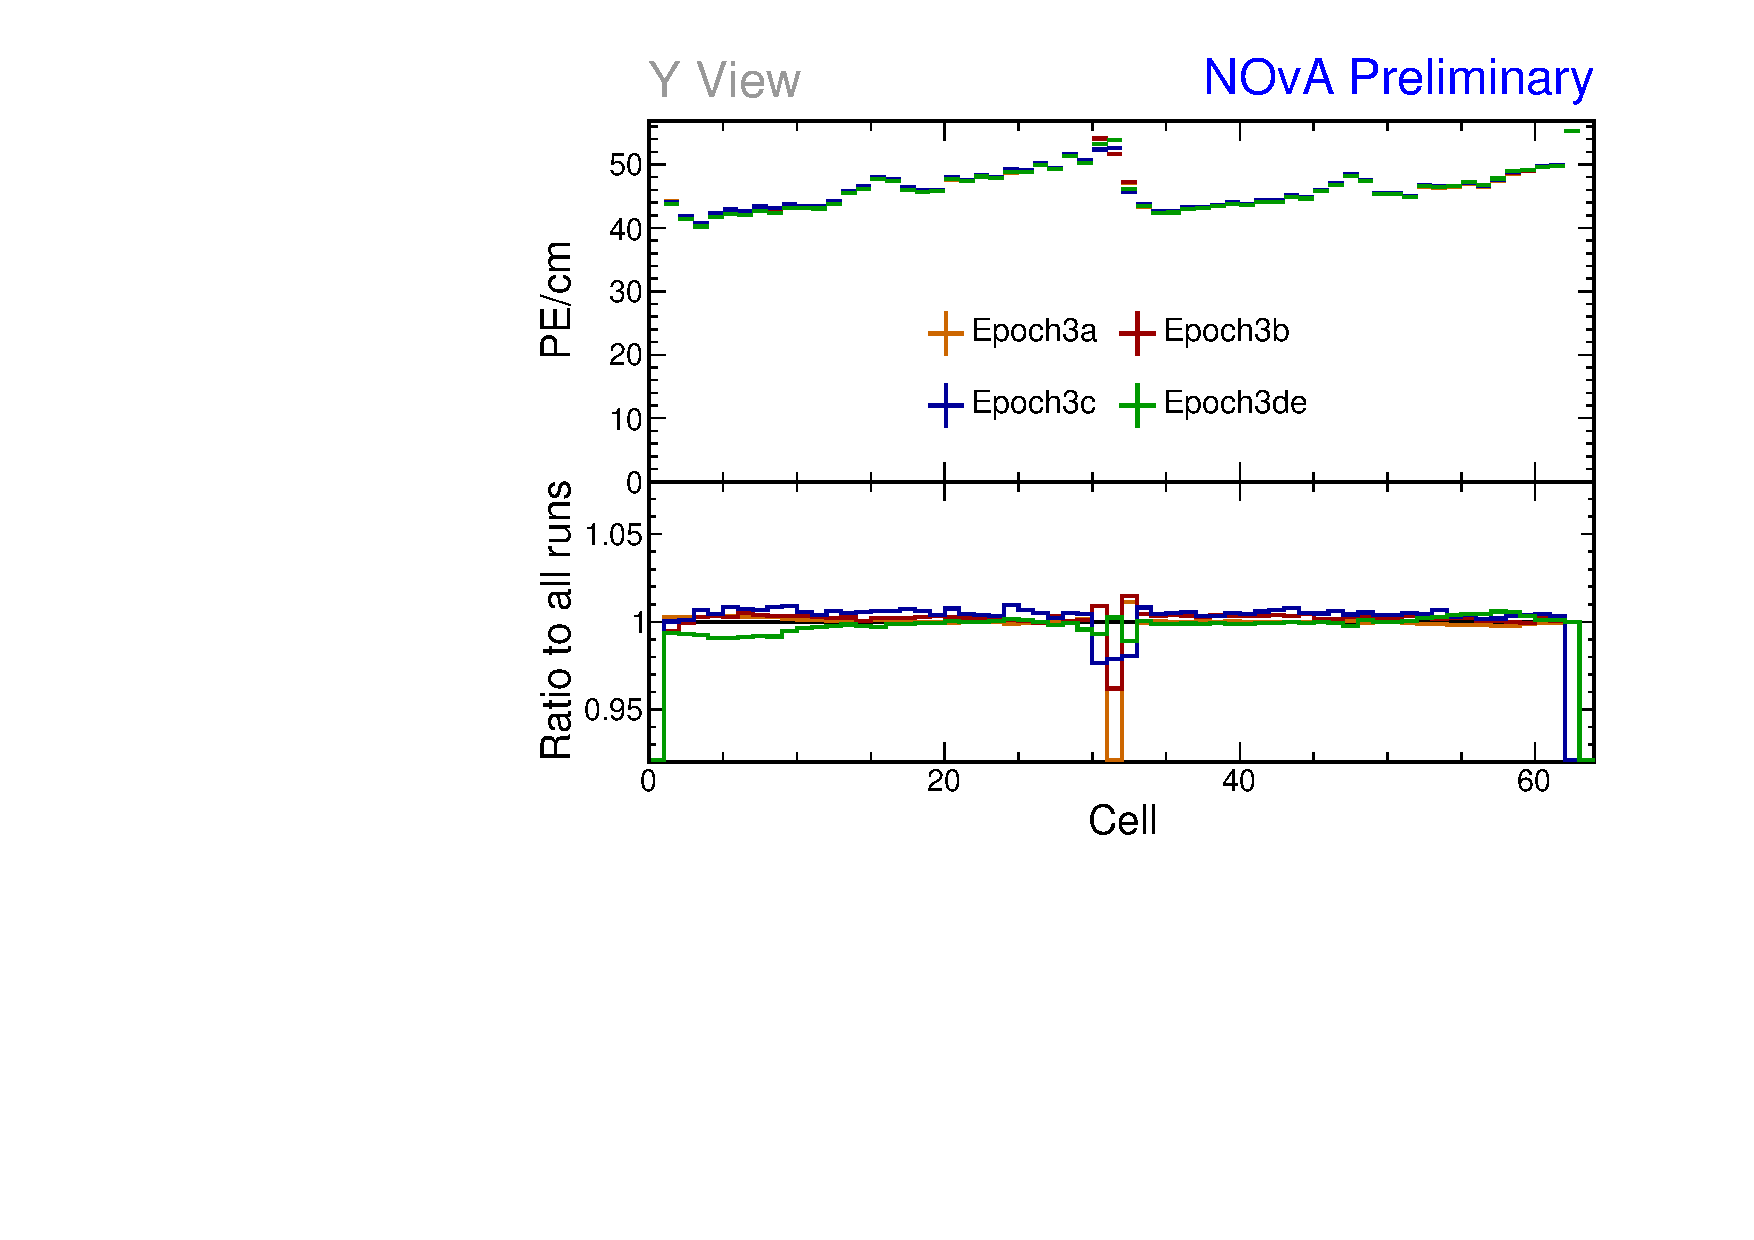
\includegraphics[width=\textwidth]{Plots/Attenprofs_P3Data_CellPE_Y_Combined.pdf}
\end{subfigure}
\caption{Uncorrected average energy response as a function of cells for epochs in period 3.}
\label{figCalibhistCellPE_period3}
\end{figure}

\begin{figure}[!hbtp]
\centering
\begin{subfigure}[b]{0.495\textwidth}
\centering
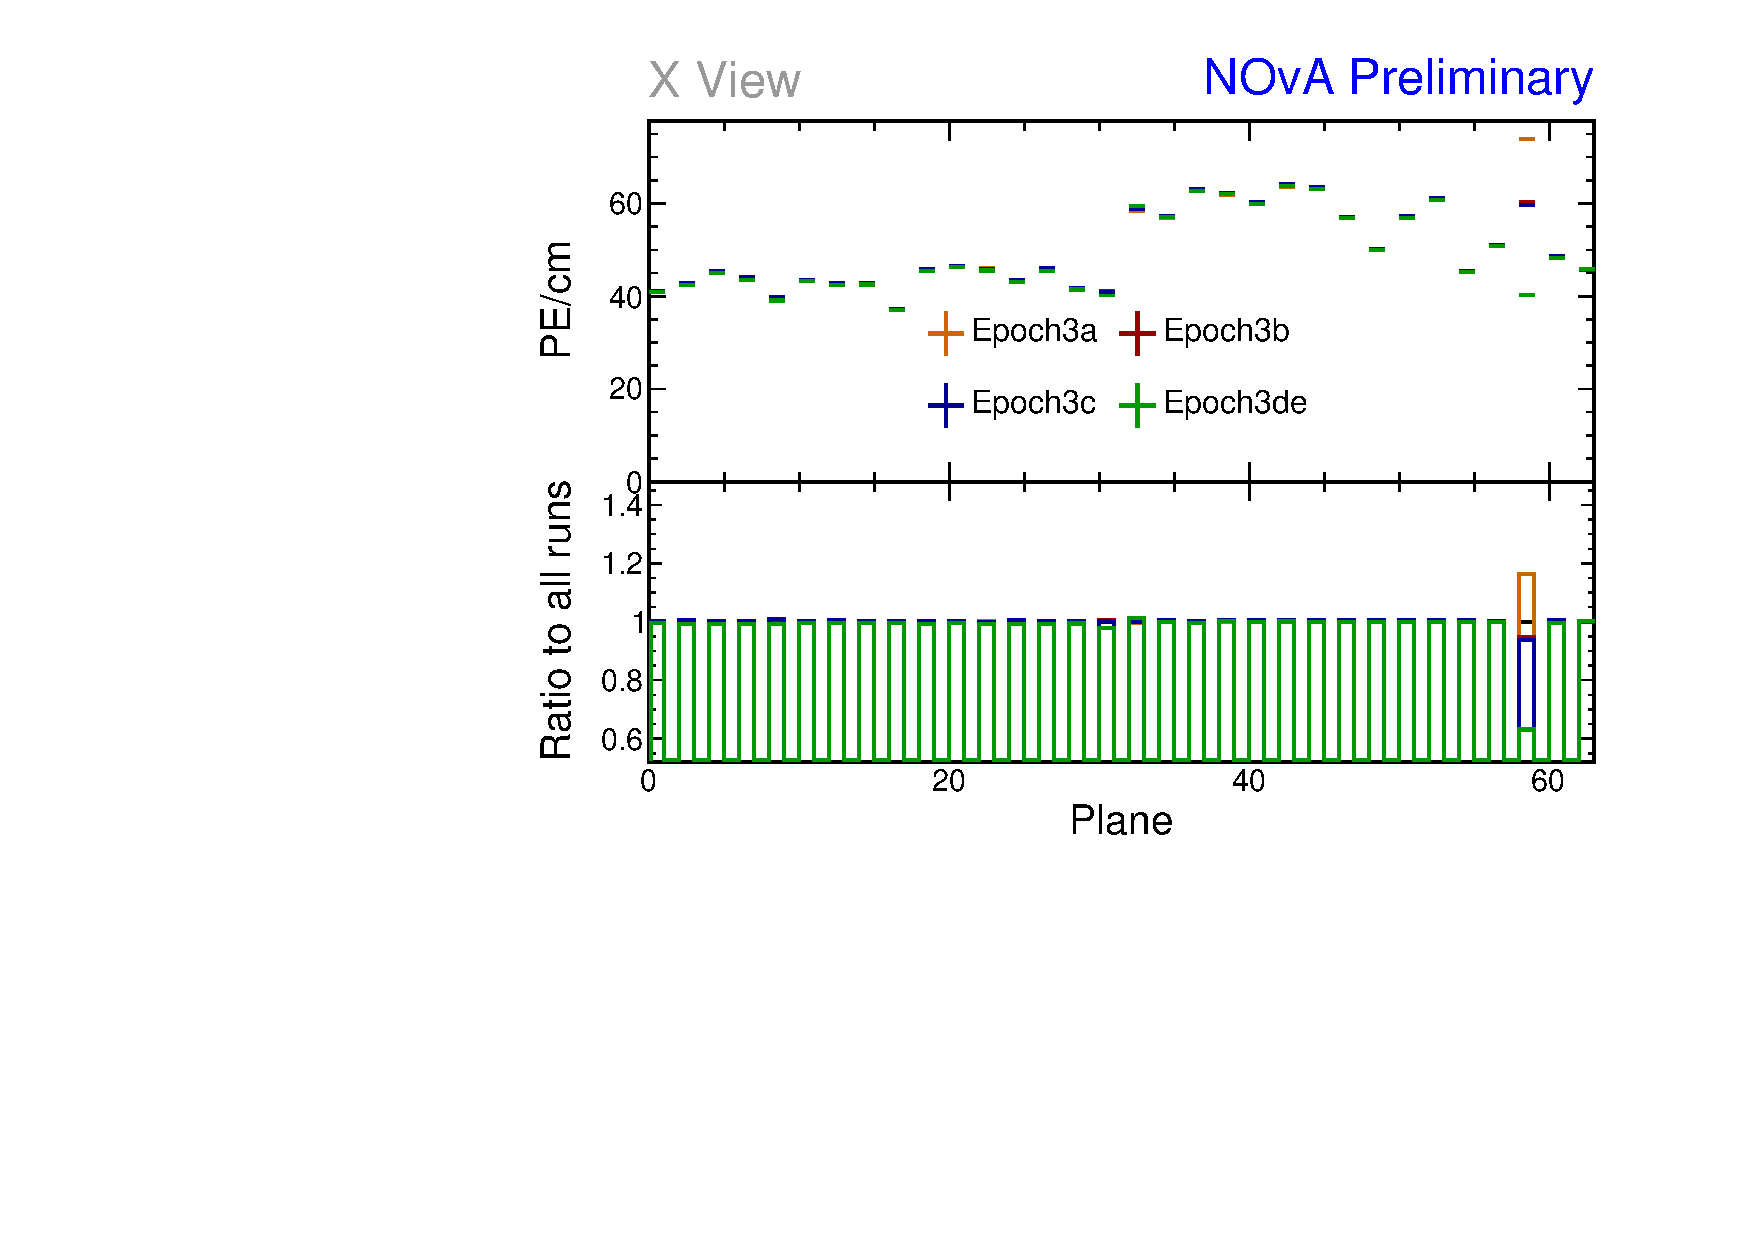
\includegraphics[width=\textwidth]{Plots/Attenprofs_P3Data_PlanePE_X_Combined.pdf}
\end{subfigure}
\begin{subfigure}[b]{0.495\textwidth}
\centering
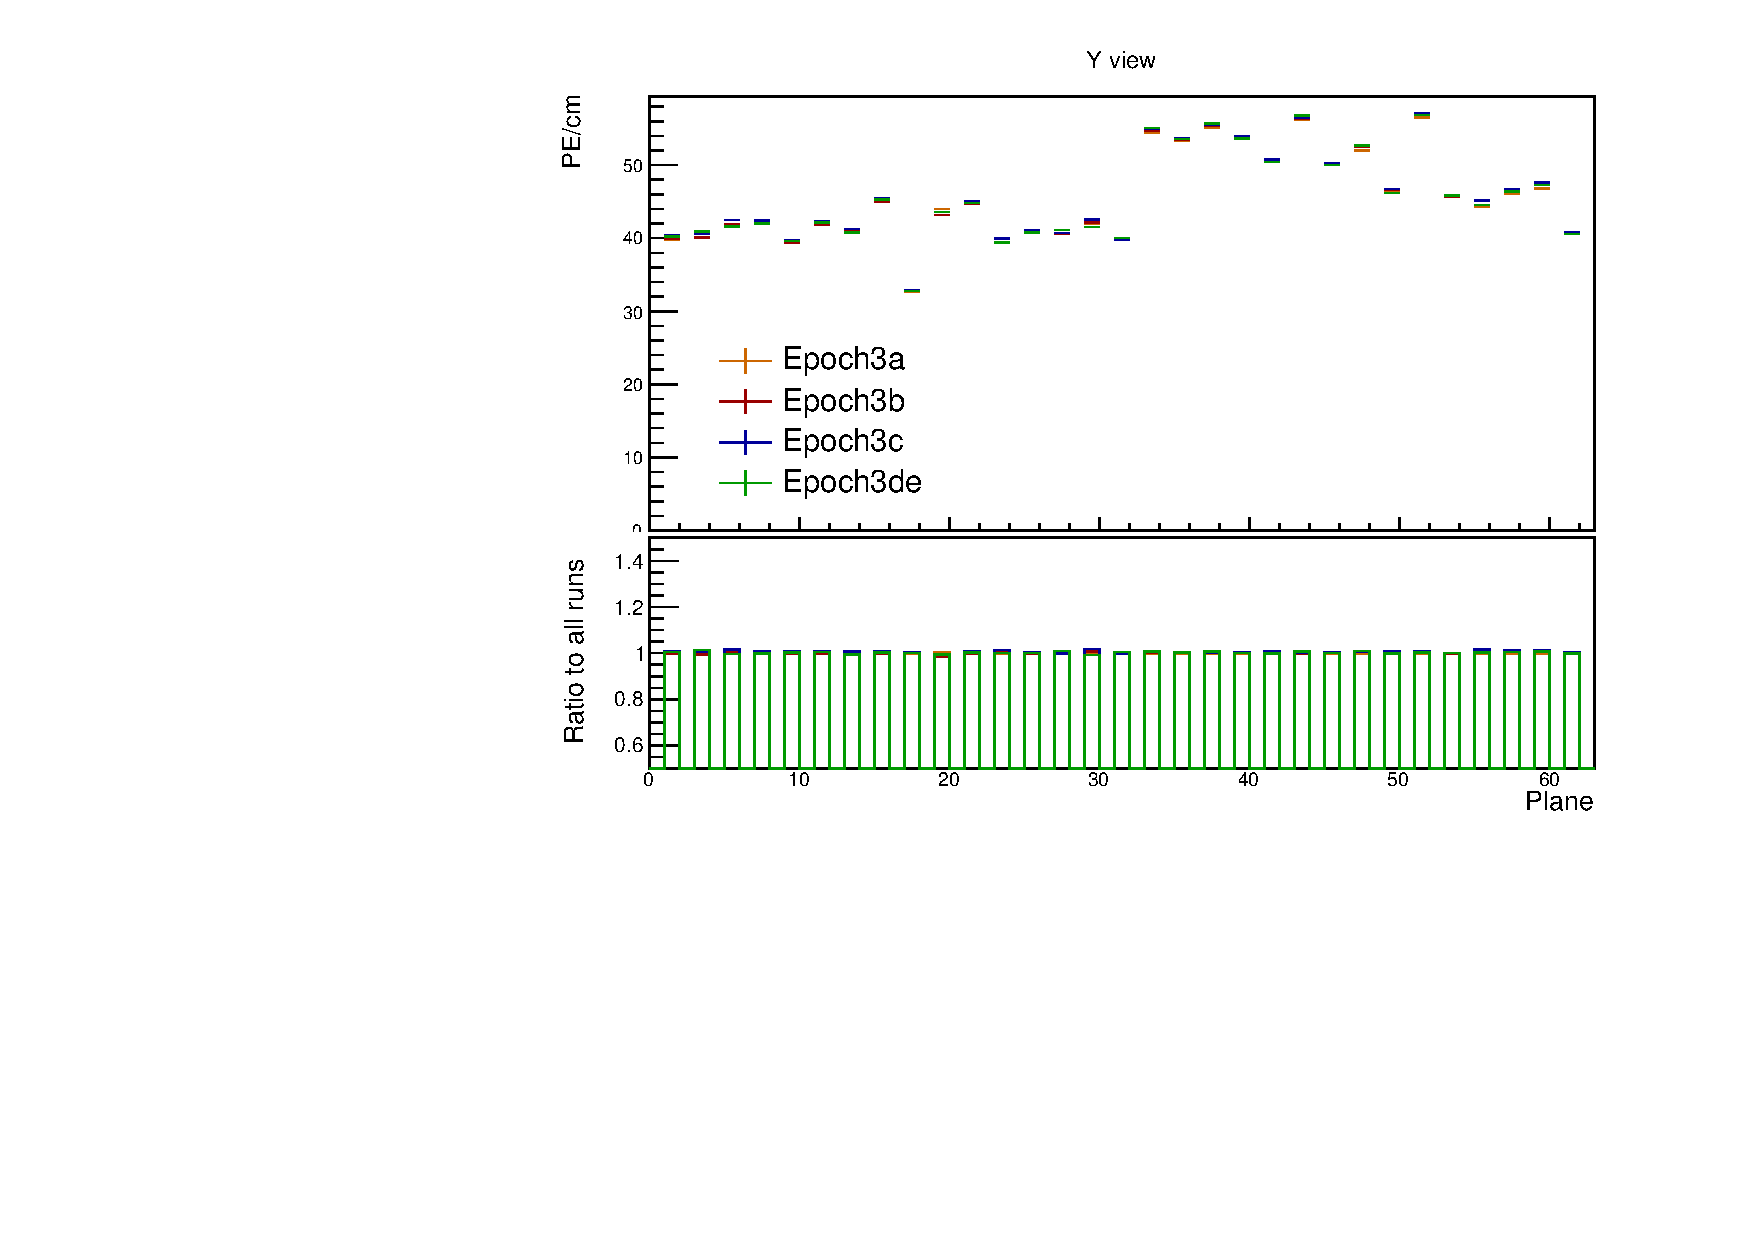
\includegraphics[width=\textwidth]{Plots/Attenprofs_P3Data_PlanePE_Y_Combined.pdf}
\end{subfigure}
\caption{Uncorrected average energy response as a function of planes for epochs in period 3.}
\label{figCalibhistPlanePE_period3}
\end{figure}

From these considerations, we decided to calibrate epochs 3a, 3b and 3c together (all epochs containing any underfilled cells) and to separately calibrate epochs 3d and 3e. The faulty FEB in the top of plane 58 is far enough in the back of the detector, that we didn't find it necessary to calibrate epochs 3d and 3e separately. Also epochs 3b and 3c only contain a few days worth of data, which wouldn't be enough for a successful attenuation fit.

\subsubsection*{Combined epochs 3a, 3b and 3c relative calibration results}

The results of the attenuation fit are summarised on Fig. \ref{figCellCentreResponseEp3abc} showing cell $\times$ plane distribution of the fitted response at the centre of each cell.

\begin{figure}[!hbtp]
\centering
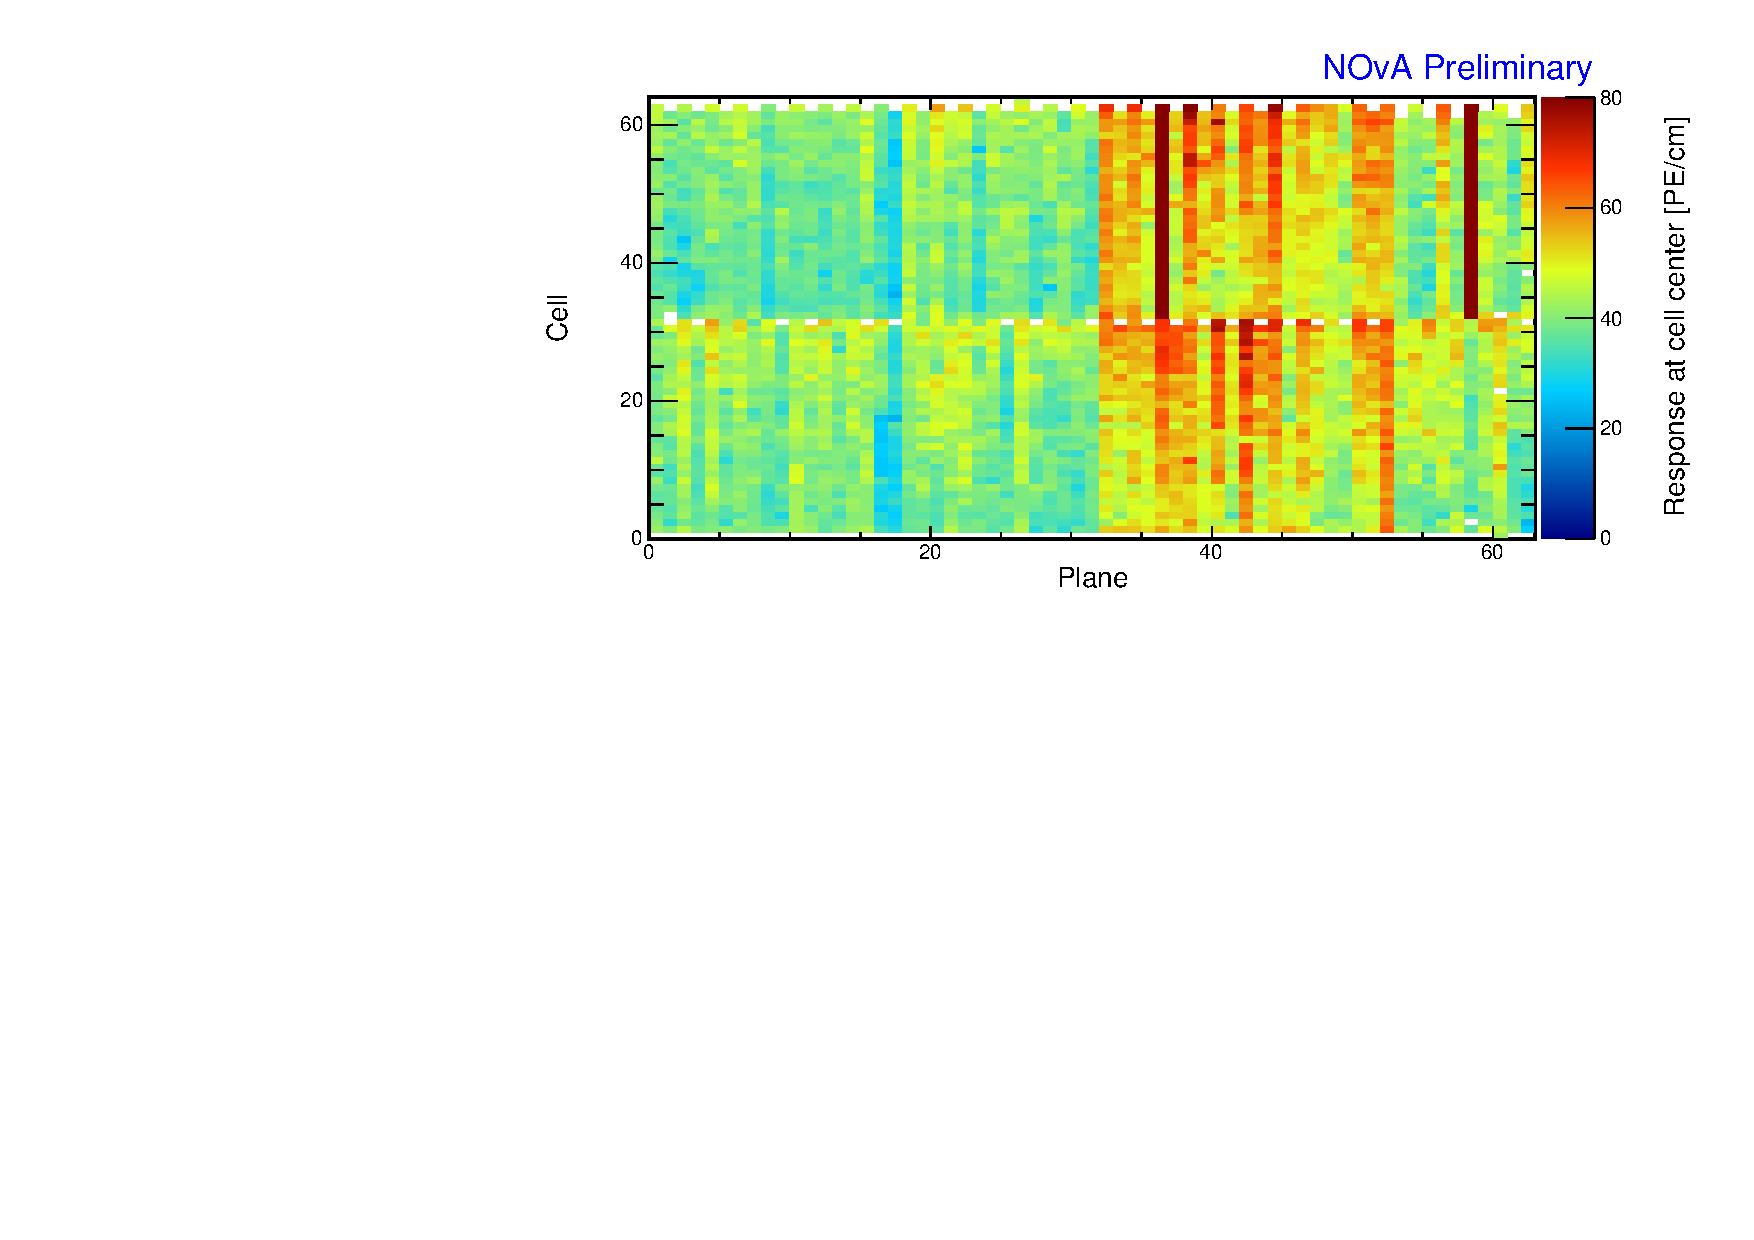
\includegraphics[width=\textwidth]{Plots/CellResponseAtCentre_epoch3abc_Limited_NOvAPlotStyle.pdf}
\caption{Overview of the relative calibration results for the Test Beam detector period 3, combined epochs 3a, 3b and 3c data. Each cell represents the result of the attenuation fit to the energy response in the centre of that cell. The blank cells are uncalibrated.}
\label{figCellCentreResponseEp3abc}
\end{figure}

We can see that some of the underfilled cells that have been refilled for epochs 3b or 3c are now calibrated thanks to including these two short epochs into the same attenuation fit. An example of energy deposition in such a cell is on the left plot of Fig. \ref{figAttenfitResultsEpoch3abc_UnderfilledCellsNeighbours}.

\begin{figure}[h]
  \begin{subfigure}{0.5\textwidth}
    \includegraphics[width=\linewidth]{RelativeCalibrationResults/ep3abc_005_031.png}
  \end{subfigure}
  \begin{subfigure}{0.5\textwidth}
    \includegraphics[width=\linewidth]{RelativeCalibrationResults/ep3abc_001_032.png}
  \end{subfigure}
  \caption{Fit to the energy response in epochs 3 a, b and c. Some underfilled cells that have been refilled in epochs 3b and 3c are now calibrated as shown on the left plot. Cell 32 in plane 1 is the only neighbouring cell to the underfilled cell that didn't manage to get calibrated due to low number of events.}
  \label{figAttenfitResultsEpoch3abc_UnderfilledCellsNeighbours}
\end{figure}

Same as in period 2, most of the neighbouring cells to the underfilled cells are calibrated, except for cell 32 in plane 1, shown on the right of Fig. \ref{figAttenfitResultsEpoch3abc_UnderfilledCellsNeighbours}. This is due to the low statistics at the edges of the detector.

There is a couple of notably faulty FEBs with a different energy response than their neighbours. Besides the expected top half of plane 58, which has about $5\times$ larger response than the usual, it's also the top half of plane 36, which has about $2.5\times$ larger response as its neighbours. This could mean that the FEB in plane 36 was faulty only for a limited time compared to the FEB in plane 58. The energy deposition for these cells is shown on Fig. \ref{figAttenfitResultsEpoch3abc_FaultyFEBs}.

\begin{figure}[h]
  \begin{subfigure}{0.5\textwidth}
    \includegraphics[width=\linewidth]{RelativeCalibrationResults/ep3abc_036_054.png}
  \end{subfigure}
  \begin{subfigure}{0.5\textwidth}
    \includegraphics[width=\linewidth]{RelativeCalibrationResults/ep3abc_058_048_ExtendedRange.png}
  \end{subfigure}
  \caption{Fit to the energy response in epochs 3a, 3b and 3c. The most obvious faulty FEBs that have a significantly larger energy response than their neighbours.}
  \label{figAttenfitResultsEpoch3abc_FaultyFEBs}
\end{figure}

Similarly as in period 2, there are a few cell in the back of the detector that have a sharp rise in the energy response at the edge of the cell, which causes them to be uncalibrated. This can be seen on Fig. \ref{figAttenfitResultsEpoch3abc_CellEdges}.

\begin{figure}[h]
  \begin{subfigure}{0.5\textwidth}
    \includegraphics[width=\linewidth]{RelativeCalibrationResults/ep3abc_058_002.png}
  \end{subfigure}
  \begin{subfigure}{0.5\textwidth}
    \includegraphics[width=\linewidth]{RelativeCalibrationResults/ep3abc_060_032.png}
  \end{subfigure}
  \caption{Fit to the energy response in epochs 3a, 3b and 3c. Some cells are not calibrated due to large fluctuations at one edge of the cells.}
  \label{figAttenfitResultsEpoch3abc_CellEdges}
\end{figure}

\subsubsection*{Combined epochs 3d and 3e relative calibration results}

The results of the attenuation fits for epochs 3d and 3e are shown on Fig. \ref{figCellCentreResponseEp3de}. There we can see the expected uncalibrated cells in plane 17 related to the dead channel (or possible still underfilled cell). The energy deposition for this cell and one of its neighbours is shown on Fig. \ref{figAttenfitResultsEpoch3de_LeftoverUnderfilledCell}.

\begin{figure}[!hbtp]
\centering
\includegraphics[width=\textwidth]{Plots/CellResponseAtCentre_epoch3de_Limited_NOvAPlotStyle.pdf}
\caption{Overview of the relative calibration results for the Test Beam detector period 3, combined epochs 3d and 3e data. Each cell represents the result of the attenuation fit to the energy response in the centre of that cell. The blank cells are uncalibrated.}
\label{figCellCentreResponseEp3de}
\end{figure}

\begin{figure}[h]
  \begin{subfigure}{0.5\textwidth}
    \includegraphics[width=\linewidth]{RelativeCalibrationResults/ep3de_017_031.png}
  \end{subfigure}
  \begin{subfigure}{0.5\textwidth}
    \includegraphics[width=\linewidth]{RelativeCalibrationResults/ep3de_017_032.png}
  \end{subfigure}
  \caption{Fit to the energy response in epochs 3d and 3e. Possibly dead channel or still underfilled cell.}
  \label{figAttenfitResultsEpoch3de_LeftoverUnderfilledCell}
\end{figure}

Epochs 3d and 3e should have all the previously underfilled cells now refilled, but as can be seen on Fig. \ref{figCellCentreResponseEp3de}, there's several of these cells that are still (officially) uncalibrated. The energy deposition in these cells is shown on Fig. \ref{figAttenfitResultsEpoch3de_RefilledDiscrepancy}. Here we can see that these cells have a fairly large discrepancy between the left and right side of the cells. This is caused by using different scintillator oils for the initial filling of the cells and for the refilling. Specifically, these cells have been initially filled with the Ash River and the Texas oils, which have higher energy depositions compared to the NDOS oil that was used for the refilling during period 3. These oils clearly didn't mix properly which causes a different energy deposition in different parts of the cells. This is a physical effect that should be accounted for in the calibration and as we can see, the attenuation fits are actually performing reasonably well. The large $\chi^2$ value is most likely caused only by the unusual shape of the distribution, which the fit is not build for. \textbf{We have therefore decided to manually change the $\chi^2$ inside the cvs tables (results of the attenuation fits), so that the $\chi^2<0.2$ and these cells are officially considered calibrated.}

\begin{figure}[h]
  \begin{subfigure}{0.5\textwidth}
    \includegraphics[width=\linewidth]{RelativeCalibrationResults/ep3de_033_031.png}
  \end{subfigure}
  \begin{subfigure}{0.5\textwidth}
    \includegraphics[width=\linewidth]{RelativeCalibrationResults/ep3de_059_031.png}
  \end{subfigure}
  \caption{Fit to the energy response in epochs 3 d and e. The scintillator oil used for refilling of the underfilled cells has lower energy response than the oil used for the initial filling. These oils didn't mix properly causing a different energy response in the left and right side of the cell.}
  \label{figAttenfitResultsEpoch3de_RefilledDiscrepancy}
\end{figure}

Some of the cells in the back of the detector have a rise, or drop in energy deposition at the edge of the cell, as can be seen on Fig. \ref{figAttenfitResultsEpoch3de_CellEdges}. This is similar to the effect seen in period 2 and epochs 3a+3b+3c and since it's again concentrated in the end of the detector, we ignored these cells and left them uncalibrated.

\begin{figure}[h]
  \begin{subfigure}{0.5\textwidth}
    \includegraphics[width=\linewidth]{RelativeCalibrationResults/ep3de_050_018.png}
  \end{subfigure}
  \begin{subfigure}{0.5\textwidth}
    \includegraphics[width=\linewidth]{RelativeCalibrationResults/ep3de_062_006.png}
  \end{subfigure}
  \caption{Fit to the energy response in epochs 3d and 3e. Some cells have a drop, or a rise of energy response at the edge of the cell. This can be cause by low statistics.}
  \label{figAttenfitResultsEpoch3de_CellEdges}
\end{figure}

\FloatBarrier
\subsection{Period 4 data}\label{secTBPeriod4}

The period 4 Test Beam data taking period is the best data we managed to collect with almost an ideal detector conditions. There's only a few commissioning runs in the very beginning of period 4, which uncovered some dead channels or faulty FEBs that were immediately fixed. These runs make up epoch 4a, shown on the top plot of Fig. \ref{figCalibhist_period4}. There is also a few runs during which we masked parts of the detector to help with FEB saturation \cite{NOVA-doc-53658}, which can clearly be seen on the middle plot of Fig. \ref{figCalibhist_period4}.

\begin{figure}[!hbtp]
\centering
\begin{subfigure}[b]{\textwidth}
\centering
\includegraphics[width=.9\textwidth]{Plots/Attenprofs_P4Data_CellPlane_Epoch4a.pdf}
\end{subfigure}
\begin{subfigure}[b]{\textwidth}
\centering
\includegraphics[width=.9\textwidth]{Plots/Attenprofs_P4Data_CellPlane_CellMasking.pdf}
\end{subfigure}
\begin{subfigure}[b]{\textwidth}
\centering
\includegraphics[width=.9\textwidth]{Plots/Attenprofs_P4Data_CellPlane_GoodRuns.pdf}
\end{subfigure}
\caption{Distribution of events in the Test Beam period 4 data calibration sample. The top plot shows the first three commissioning runs, the middle plot the status of the detector during the Cell Masking studies and the bottom plot shows the rest.}
\label{figCalibhist_period4}
\end{figure}

Figures \ref{figCalibhistWPE_period4}, \ref{figCalibhistCellPE_period4} and \ref{figCalibhistPlanePE_period4} show that the epoch 4a and the cell masking study did have a noticeable impact on the energy deposition across the detector. We have therefore decided to ignore these runs and only calibrate the rest of the period 4 data.

\begin{figure}[!hbtp]
\centering
\begin{subfigure}[b]{0.495\textwidth}
\centering
\includegraphics[width=\textwidth]{Plots/Attenprofs_P4Data_WPE_corr_xy_X_Combined.pdf}
\end{subfigure}
\begin{subfigure}[b]{0.495\textwidth}
\centering
\includegraphics[width=\textwidth]{Plots/Attenprofs_P4Data_WPE_corr_xy_Y_Combined.pdf}
\end{subfigure}
\caption{Uncorrected average energy response as a function of the position within a cell (w) for epochs in period 4.}
\label{figCalibhistWPE_period4}
\end{figure}

\begin{figure}[!hbtp]
\centering
\begin{subfigure}[b]{0.495\textwidth}
\centering
\includegraphics[width=\textwidth]{Plots/Attenprofs_P4Data_CellPE_X_Combined.pdf}
\end{subfigure}
\begin{subfigure}[b]{0.495\textwidth}
\centering
\includegraphics[width=\textwidth]{Plots/Attenprofs_P4Data_CellPE_Y_Combined.pdf}
\end{subfigure}
\caption{Uncorrected average energy response as a function of cells for epochs in period 4.}
\label{figCalibhistCellPE_period4}
\end{figure}

\begin{figure}[!hbtp]
\centering
\begin{subfigure}[b]{0.495\textwidth}
\centering
\includegraphics[width=\textwidth]{Plots/Attenprofs_P4Data_PlanePE_X_Combined.pdf}
\end{subfigure}
\begin{subfigure}[b]{0.495\textwidth}
\centering
\includegraphics[width=\textwidth]{Plots/Attenprofs_P4Data_PlanePE_Y_Combined.pdf}
\end{subfigure}
\caption{Uncorrected average energy response as a function of planes for epochs in period 4.}
\label{figCalibhistPlanePE_period4}
\end{figure}

\subsubsection*{Period 4 relative calibration results}

Results of the attenuation fits for period 4 are summarised on Fig. \ref{figCellCentreResponsePeriod4}. We can see that majority of the detector is calibrated, besides some cells on the edge of the detector, a few formerly underfilled cells (left plot on Fig. \ref{figAttenfitResultsPeriod4}), and one cell with an unusually high response at the edge of the cell (right plot on Fig. \ref{figAttenfitResultsPeriod4}).

\begin{figure}[!hbtp]
\centering
\includegraphics[width=\textwidth]{Plots/CellResponseAtCentre_period4_Limited_NOvAPlotStyle.pdf}
\caption{Overview of the relative calibration results for the Test Beam detector period 4 data. Each cell represents the result of the attenuation fit to the energy response in the centre of that cell. The blank cells are uncalibrated.}
\label{figCellCentreResponsePeriod4}
\end{figure}

We treated the formerly underfilled cells the same way as in epochs 3d and 3e, by manually changing their $\chi^2$ inside the csv files to be $<0.2$ and therefore making them officially calibrated.

\begin{figure}[h]
  \begin{subfigure}{0.5\textwidth}
    \includegraphics[width=\linewidth]{RelativeCalibrationResults/p4_035_031.png}
  \end{subfigure}
  \begin{subfigure}{0.5\textwidth}
    \includegraphics[width=\linewidth]{RelativeCalibrationResults/p4_054_047.png}
  \end{subfigure}
  \caption{Fit to the energy response in period 4. Previously underfilled cells refilled with a scintillator of a different quality causing an unusual distribution of energy deposition (left). Unusually high energy response at the edge of the cell 47 (right).}
  \label{figAttenfitResultsPeriod4}
\end{figure}

\FloatBarrier
%%%%%%%%%%%%%%%%%%%%%%%%%%%%%%%%%%%%%%%%%%%%%%%%%%%%%%%%%%%%%%%%%%%%%%%%%%%%%%%
%%%%%%%%%%%%%%%%%%%%%%%%%%%%%%%%%%%%%%%%%%%%%%%%%%%%%%%%%%%%%%%%%%%%%%%%%%%%%%%
%%%
%%%                        Absolute calibration results
%%%
%%%%%%%%%%%%%%%%%%%%%%%%%%%%%%%%%%%%%%%%%%%%%%%%%%%%%%%%%%%%%%%%%%%%%%%%%%%%%%%
\subsection{Absolute calibration results}
To get the absolute energy scale we look at the stopping muon sample, apply the relative calibration results and the absolute calibration cuts to select only well-understood minimum ionising muons. The absolute calibration cuts are mostly the same as for the other detectors (hits 1-2 m from the end of track, $\unit{pathlength}>0$, $\unit{PE}>0$, $\unit{PECorr} > 0$, $\unit{PECorr/cm} < 100$), but with a smaller cell window $-80<w<80\ \unit{cm}$ to remove hits at the cell edges.

We then look at the distributions of the reconstructed energy response in units of $\unit{PECorr/cm}$ (for all data and simulation samples), and true energy response in units of $\unit{MeV/cm}$ (only for simulation) in each view, as shown on Fig. \ref{figAbsCalibMEU}. The mean of these distributions is the $\textsf{MEU}_{Reco/True}$ value for each view, with an uncertainty calculated as $StdDev/\sqrt{N_{Entries}}$ from the distribution. The $\textsf{MEU}$ for each sample and view is shown on table \ref{tab:calib_summary_table}.

\begin{figure}[!hbtp]
\centering
\begin{subfigure}[b]{0.495\textwidth}
\centering
\includegraphics[width=\textwidth]{Plots/Period4_nhits_meu_y.pdf}
\end{subfigure}
\begin{subfigure}[b]{0.495\textwidth}
\centering
\includegraphics[width=\textwidth]{Plots/MC_nhits_mev_y.pdf}
\end{subfigure}
\caption{Example distributions of reconstructed (left) and true (right) energy response of stopping muons 1-2 m from the end of their tracks. The mean of the reconstructed (true) response is the reconstructed (true) MEU unit.}
\label{figAbsCalibMEU}
\end{figure}

\begin{table}[h!]
\centering
\begin{tabular}{|c|c|c|c|c|c|c|c|}
\hline
\multicolumn{2}{|c|}{\multirow{2}{*}{Sample}} & \multicolumn{2}{c|}{X view} & \multicolumn{2}{c|}{Y view} & \multicolumn{2}{c|}{Combined}\\\cline{3-8}
\multicolumn{2}{|c|}{} & NHits & MEU & NHits & MEU & \cellcolor[HTML]{F8A102}MEU$_{Reco}$ & $\sigma_{\textsf{MEU}_{Reco}}$\\ \hline
 \parbox[t]{2mm}{\multirow{4}{*}{\rotatebox[origin=c]{90}{Data}}}
 & Period 2 & 2.322e+05 & 38.70 & 1.413e+06 & 39.40 & \cellcolor[HTML]{F8A102}39.05 & 0.02\\ \cline{2-8} 
 & Epochs 3abc & 2.638e+05 & 38.49 & 1.621e+06 & 39.40 & \cellcolor[HTML]{F8A102}38.94 & 0.02\\ \cline{2-8}
 & Epochs 3de & 1.049e+05 & 38.63 & 6.725e+05 & 39.42 & \cellcolor[HTML]{F8A102}39.02 & 0.03\\ \cline{2-8}
 & Period 4 & 5.268e+05 & 38.63 & 3.316e+06 & 39.40 & \cellcolor[HTML]{F8A102}39.01 & 0.01\\ \hline
\multicolumn{2}{|c|}{Simulation} & 2.829e+05 & 40.17 & 1.842e+06 & 39.93 & \cellcolor[HTML]{F8A102}40.05 & 0.02\\ \hline
\end{tabular}

\vspace*{2mm}
\begin{tabular}{|c|c|}
\hline
\cellcolor[HTML]{F8A102}MEU$_{True}$ = 1.7722 $\unit{MeV/cm}$ & $\sigma_{\textsf{MEU}_{True}}$ = 0.0003 $\unit{MeV/cm}$\\ \hline
\end{tabular}
\caption{Table of the absolute calibration results. MEU$_{Reco}$ values (top table) are in units of $\unit{PECorr/cm}$ and MEU$_{True}$ values (bottom table) are in units of $\unit{MeV/cm}$}
\label{tab:calib_summary_table}
\end{table}

We don't apply the absolute energy scale separately for each view, instead we combine the two views into a single $\textsf{MEU}_{Reco}$, or $\textsf{MEU}_{True}$ value. To combine the $\textsf{MEU}$ value we take a simple average $\left(\textsf{MEU}_X+\textsf{MEU}_Y\right)/2$, without accounting for the different statistics of the two views. To get the uncertainty on the final value, we calculate it as $\sigma^2_{Combined}=\sigma^2_{X} + \sigma^2_Y$. In the past (and for the other NOvA detectors), this uncertainty was calculated as $1/\sigma^2_{Combined}=1/\sigma^2_{X} + 1/\sigma^2_Y$. This uncertainty is however \textbf{not} the uncertainty used in NOvA for the absolute energy scale. Instead, we use a data-simulation comparison of special special samples to derive an uncertainty on the absolute energy scale \cite{NOVA-doc-36915}. The final combined values are highlighted in table \ref{tab:calib_summary_table}. Here $\textsf{MEU}_{Reco}$ values are all in units of $\unit{PECorr/cm}$.

For each calibrated sample we write the combined $\textsf{MEU}_{Reco}$ value into an \texttt{calib\_abs\_consts.csv} file, together with its uncertainty and with the $\textsf{MEU}_{True}$ value, which is common for all samples.

%%%%%%%%%%%%%%%%%%%%%%%%%%%%%%%%%%%%%%%%%%%%%%%%%%%%%%%%%%%%%%%%%%%%%%%%%%%%%%%
%%%%%%%%%%%%%%%%%%%%%%%%%%%%%%%%%%%%%%%%%%%%%%%%%%%%%%%%%%%%%%%%%%%%%%%%%%%%%%%
%%%
%%%                      Final results and conclusions
%%%
%%%%%%%%%%%%%%%%%%%%%%%%%%%%%%%%%%%%%%%%%%%%%%%%%%%%%%%%%%%%%%%%%%%%%%%%%%%%%%%
\subsection{Results}
The results of the relative and the absolute calibration, in form of the csv files, are stored in \texttt{/grid/fermiapp/products/nova/externals/calibcsvs/} and are applied within NOvASoft in the calibration tag v15.09 and higher.

The \texttt{csv} files follow the official NOvA calibration naming convention, which is \\\texttt{calib\_\{abs/atten\}\_\{consts/points\}.\{nd/fd/tb\}.\{data/mc\}.\{version\}.\{period\}.csv}. Here \texttt{version} is the calibration tag (i.e. v15) and period is the range of runs for that sample (i.e. \texttt{r100857-r101356} for the combined epochs 3a, 3b, and 3c, or \texttt{r-r} for simulation, since it is not divided into different periods).

To create the calibration tag we've asked Lisa Koerner for help. Lisa is a NOvA calibration expert who wrote the instructions for calibration tagging \cite{NOVA-doc-59268}. It is possible to do it ourselves following these instructions, but it is advised to consult the detector systematics group before hand.

We have also stored the final calibration results in a special location created for safekeeping of Test Beam calibration files: \texttt{/nova/ana/testbeam/calibration}. Here we have also copied all of the attenuation profiles used in the relative calibration. These can be very useful in case someone wants to re-do the calibration, as it allows to skip the prestaging of the calibration pclist samples (the pcliststop samples are much smaller and therefore easier to prestage). If there has been no change to the calibration samples, it is possible to skip the creation of attenuation profiles and reuse the existing files.

\subsection{Validation}
To validate the results of the Test Beam calibration we look at the stopping muon sample used for the absolute calibration, since these events have the most consistent and reliable energy deposition.

In plots on Fig. \ref{figAbsCalibW1}-\ref{figAbsCalibDrift2} we look at distributions of variables used during the calibration, namely $PE$, $PECorr$, $Pathlength$, $PE/cm$ and $PECorr/cm$. Their distributions are over a range of variables we tried to correct the energy deposition in, namely position within a cell $w$, cell number, plane number, track angles and time.

The most important validation plots are the distributions of $PECorr/cm$, which should be completely flat. This would mean that all the deposited energy results in an equivalent recorded energy wherever and whenever in the Test Beam detector it occurred. As can be seen on the validation plots, this was successfully achieved and the $PECorr/cm$ distributions are mostly flat across all studied variables.

The distribution of $PECorr/cm$ across cells in X view on Fig. \ref{figAbsCalibPlane1} seems fairly scattered, however this is mostly due to the better resolution of this plot and the dispersion of the energy deposition across cells isn't large enough to constitute further investigation.

The distributions of $PECorr/cm$ across planes in the X view (Fig. \ref{figAbsCalibPlane1}) shows a noticeable smaller corrected energy response of stopping muons in plane 36. This means that the relative calibration over-corrected the energy response due to the through-going muons having unusually high energy response (as shown on Fig. \ref{figAttenfitResultsEpoch3abc_FaultyFEBs}), but not the selected stopping muons. The most likely cause is that the impacted FEB was "faulty" only for a certain period of time. In that case the corrected energy response would be correct for the period when the FEB was faulty, but would be under-estimated for the period when the FEB behaved "normally". The $PECorr/cm$ over Plane plot shows the average over these responses.

The corrected response across planes in Y view (Fig. \ref{figAbsCalibPlane1}) shows a slight incline in the first half of the detector. We do not know where does this slope come from, but it is not big enough to be of concern and we decided to ignore it.

The distributions of energy deposition in time (Fig. \ref{figAbsCalibDrift1} and \ref{figAbsCalibDrift2}) show a non-trivial dependency. The detector response could be influenced by environmental factors (temperature and humidity) and by scintillator or readout ageing. Neither of these factors are well understood within NOvA and Test Beam detector could be potentially used to shine more light on this issue. However this is a topic for a separate study and is out of scope of this technical note.

Technically, we would expect the distributions of $PECorr/cm$ to also have the same \textbf{scale} for all data samples and for simulation. As can be seen on all the validation plots, the data samples have a reasonably similar scale of $PECorr/cm$, but this is noticeably different for simulation. This is caused due to the data-based simulation we are using does not have a correct energy estimation for through-going muons, which have generally underestimated energies \cite{NOVA-doc-60026}. This results in an over-estimated correction from the relative calibration. However, this is not an issue, since we only use stopping muons to calculate the absolute energy scale and stopping muons have correct energies in the new simulation.

\begin{figure}[!ht]
  \begin{subfigure}{\textwidth}
  \centering
    \includegraphics[height=0.2\linewidth]{essentialsec_tb/legend.pdf}
  \end{subfigure}
  \vspace*{2mm}
  
  \begin{subfigure}{0.5\textwidth}
    \includegraphics[width=\linewidth]{essentialsec_tb/pecm_w_x.pdf}
  \end{subfigure}
  \begin{subfigure}{0.5\textwidth}
    \includegraphics[width=\linewidth]{essentialsec_tb/pecm_w_y.pdf}
  \end{subfigure}
  \begin{subfigure}{0.5\textwidth}
    \includegraphics[width=\linewidth]{essentialsec_tb/pecorrcm_w_x.pdf}
  \end{subfigure}
  \begin{subfigure}{0.5\textwidth}
    \includegraphics[width=\linewidth]{essentialsec_tb/pecorrcm_w_y.pdf}
  \end{subfigure}
  \caption{Distributions of stopping muons within a 1-2 m track window from the end of their tracks across the position within a cell.}
  \label{figAbsCalibW1}
\end{figure}

\begin{figure}[!ht]
  \begin{subfigure}{\textwidth}
  \centering
    \includegraphics[height=0.2\linewidth]{essentialsec_tb/legend.pdf}
  \end{subfigure}
  \vspace*{2mm}

  \begin{subfigure}{0.5\textwidth}
    \includegraphics[width=\linewidth]{essentialsec_tb/pe_w_x.pdf}
  \end{subfigure}
  \begin{subfigure}{0.5\textwidth}
    \includegraphics[width=\linewidth]{essentialsec_tb/pe_w_y.pdf}
  \end{subfigure}
  \begin{subfigure}{0.5\textwidth}
    \includegraphics[width=\linewidth]{essentialsec_tb/pecorr_w_x.pdf}
  \end{subfigure}
  \begin{subfigure}{0.5\textwidth}
    \includegraphics[width=\linewidth]{essentialsec_tb/pecorr_w_y.pdf}
  \end{subfigure}
  \begin{subfigure}{0.5\textwidth}
    \includegraphics[width=\linewidth]{essentialsec_tb/cm_w_x.pdf}
  \end{subfigure}
  \begin{subfigure}{0.5\textwidth}
    \includegraphics[width=\linewidth]{essentialsec_tb/cm_w_y.pdf}
  \end{subfigure}
  \caption{Distributions of stopping muons within a 1-2 m track window from the end of their tracks across the position within a cell.}
  \label{figAbsCalibW2}
\end{figure}

\begin{figure}[!ht]
  \begin{subfigure}{\textwidth}
  \centering
    \includegraphics[height=0.2\linewidth]{essentialsec_tb/legend.pdf}
  \end{subfigure}
  \vspace*{2mm}

  \begin{subfigure}{0.5\textwidth}
    \includegraphics[width=\linewidth]{essentialsec_tb/pecm_cell_x.pdf}
  \end{subfigure}
  \begin{subfigure}{0.5\textwidth}
    \includegraphics[width=\linewidth]{essentialsec_tb/pecm_cell_y.pdf}
  \end{subfigure}
  \begin{subfigure}{0.5\textwidth}
    \includegraphics[width=\linewidth]{essentialsec_tb/pecorrcm_cell_x.pdf}
  \end{subfigure}
  \begin{subfigure}{0.5\textwidth}
    \includegraphics[width=\linewidth]{essentialsec_tb/pecorrcm_cell_y.pdf}
  \end{subfigure}
  \caption{Distributions of stopping muons within a 1-2 m track window from the end of their tracks across the cells of the detector.}
  \label{figAbsCalibCell1}
\end{figure}

\begin{figure}[!ht]
  \begin{subfigure}{\textwidth}
  \centering
    \includegraphics[height=0.2\linewidth]{essentialsec_tb/legend.pdf}
  \end{subfigure}
  \vspace*{2mm}

  \begin{subfigure}{0.5\textwidth}
    \includegraphics[width=\linewidth]{essentialsec_tb/pe_cell_x.pdf}
  \end{subfigure}
  \begin{subfigure}{0.5\textwidth}
    \includegraphics[width=\linewidth]{essentialsec_tb/pe_cell_y.pdf}
  \end{subfigure}
  \begin{subfigure}{0.5\textwidth}
    \includegraphics[width=\linewidth]{essentialsec_tb/pecorr_cell_x.pdf}
  \end{subfigure}
  \begin{subfigure}{0.5\textwidth}
    \includegraphics[width=\linewidth]{essentialsec_tb/pecorr_cell_y.pdf}
  \end{subfigure}
  \begin{subfigure}{0.5\textwidth}
    \includegraphics[width=\linewidth]{essentialsec_tb/cm_cell_x.pdf}
  \end{subfigure}
  \begin{subfigure}{0.5\textwidth}
    \includegraphics[width=\linewidth]{essentialsec_tb/cm_cell_y.pdf}
  \end{subfigure}
  \caption{Distributions of stopping muons within a 1-2 m track window from the end of their tracks across the cells of the detector.}
  \label{figAbsCalibCell2}
\end{figure}

\begin{figure}[!ht]
  \begin{subfigure}{\textwidth}
  \centering
    \includegraphics[height=0.2\linewidth]{essentialsec_tb/legend.pdf}
  \end{subfigure}
  \vspace*{2mm}

  \begin{subfigure}{0.5\textwidth}
    \includegraphics[width=\linewidth]{essentialsec_tb/pecm_plane_x.pdf}
  \end{subfigure}
  \begin{subfigure}{0.5\textwidth}
    \includegraphics[width=\linewidth]{essentialsec_tb/pecm_plane_y.pdf}
  \end{subfigure}
  \begin{subfigure}{0.5\textwidth}
    \includegraphics[width=\linewidth]{essentialsec_tb/pecorrcm_plane_x.pdf}
  \end{subfigure}
  \begin{subfigure}{0.5\textwidth}
    \includegraphics[width=\linewidth]{essentialsec_tb/pecorrcm_plane_y.pdf}
  \end{subfigure}
  \caption{Distributions of stopping muons within a 1-2 m track window from the end of their tracks across the planes of the detector.}
  \label{figAbsCalibPlane1}
\end{figure}

\begin{figure}[!ht]
  \begin{subfigure}{\textwidth}
  \centering
    \includegraphics[height=0.2\linewidth]{essentialsec_tb/legend.pdf}
  \end{subfigure}
  \vspace*{2mm}

  \begin{subfigure}{0.5\textwidth}
    \includegraphics[width=\linewidth]{essentialsec_tb/pe_plane_x.pdf}
  \end{subfigure}
  \begin{subfigure}{0.5\textwidth}
    \includegraphics[width=\linewidth]{essentialsec_tb/pe_plane_y.pdf}
  \end{subfigure}
  \begin{subfigure}{0.5\textwidth}
    \includegraphics[width=\linewidth]{essentialsec_tb/pecorr_plane_x.pdf}
  \end{subfigure}
  \begin{subfigure}{0.5\textwidth}
    \includegraphics[width=\linewidth]{essentialsec_tb/pecorr_plane_y.pdf}
  \end{subfigure}
  \begin{subfigure}{0.5\textwidth}
    \includegraphics[width=\linewidth]{essentialsec_tb/cm_plane_x.pdf}
  \end{subfigure}
  \begin{subfigure}{0.5\textwidth}
    \includegraphics[width=\linewidth]{essentialsec_tb/cm_plane_y.pdf}
  \end{subfigure}
  \caption{Distributions of stopping muons within a 1-2 m track window from the end of their tracks across the planes of the detector.}
  \label{figAbsCalibPlane2}
\end{figure}

\begin{figure}[!ht]
  \begin{subfigure}{\textwidth}
  \centering
    \includegraphics[height=0.2\linewidth]{essentialsec_tb/legend.pdf}
  \end{subfigure}
  \vspace*{2mm}

  \begin{subfigure}{0.5\textwidth}
    \includegraphics[width=\linewidth]{PlotsAngularDistribution/pecm_cosx_x.pdf}
  \end{subfigure}
  \begin{subfigure}{0.5\textwidth}
    \includegraphics[width=\linewidth]{PlotsAngularDistribution/pecm_cosx_y.pdf}
  \end{subfigure}
  \begin{subfigure}{0.5\textwidth}
    \includegraphics[width=\linewidth]{PlotsAngularDistribution/pecorrcm_cosx_x.pdf}
  \end{subfigure}
  \begin{subfigure}{0.5\textwidth}
    \includegraphics[width=\linewidth]{PlotsAngularDistribution/pecorrcm_cosx_y.pdf}
  \end{subfigure}
  \caption{Distributions of stopping muons within a 1-2 m track window from the end of their tracks across the cosine of the track angle from the X (horizontal) axis.}
  \label{figAbsCalibCosX1}
\end{figure}

\begin{figure}[!ht]
  \begin{subfigure}{\textwidth}
  \centering
    \includegraphics[height=0.2\linewidth]{essentialsec_tb/legend.pdf}
  \end{subfigure}
  \vspace*{2mm}

  \begin{subfigure}{0.5\textwidth}
    \includegraphics[width=\linewidth]{PlotsAngularDistribution/pe_cosx_x.pdf}
  \end{subfigure}
  \begin{subfigure}{0.5\textwidth}
    \includegraphics[width=\linewidth]{PlotsAngularDistribution/pe_cosx_y.pdf}
  \end{subfigure}
  \begin{subfigure}{0.5\textwidth}
    \includegraphics[width=\linewidth]{PlotsAngularDistribution/pecorr_cosx_x.pdf}
  \end{subfigure}
  \begin{subfigure}{0.5\textwidth}
    \includegraphics[width=\linewidth]{PlotsAngularDistribution/pecorr_cosx_y.pdf}
  \end{subfigure}
  \begin{subfigure}{0.5\textwidth}
    \includegraphics[width=\linewidth]{PlotsAngularDistribution/cm_cosx_x.pdf}
  \end{subfigure}
  \begin{subfigure}{0.5\textwidth}
    \includegraphics[width=\linewidth]{PlotsAngularDistribution/cm_cosx_y.pdf}
  \end{subfigure}
  \caption{Distributions of stopping muons within a 1-2 m track window from the end of their tracks across the cosine of the track angle from the X (horizontal) axis.}
  \label{figAbsCalibCosX2}
\end{figure}

\begin{figure}[!ht]
  \begin{subfigure}{\textwidth}
  \centering
    \includegraphics[height=0.2\linewidth]{essentialsec_tb/legend.pdf}
  \end{subfigure}
  \vspace*{2mm}
  
  \begin{subfigure}{0.5\textwidth}
    \includegraphics[width=\linewidth]{PlotsAngularDistribution/pecm_cosy_x.pdf}
  \end{subfigure}
  \begin{subfigure}{0.5\textwidth}
    \includegraphics[width=\linewidth]{PlotsAngularDistribution/pecm_cosy_y.pdf}
  \end{subfigure}
  \begin{subfigure}{0.5\textwidth}
    \includegraphics[width=\linewidth]{PlotsAngularDistribution/pecorrcm_cosy_x.pdf}
  \end{subfigure}
  \begin{subfigure}{0.5\textwidth}
    \includegraphics[width=\linewidth]{PlotsAngularDistribution/pecorrcm_cosy_y.pdf}
  \end{subfigure}
  \caption{Distributions of stopping muons within a 1-2 m track window from the end of their tracks across the cosine of the track angle from the Y (vertical) axis.}
  \label{figAbsCalibCosY1}
\end{figure}

\begin{figure}[!ht]
  \begin{subfigure}{\textwidth}
  \centering
    \includegraphics[height=0.2\linewidth]{essentialsec_tb/legend.pdf}
  \end{subfigure}
  \vspace*{2mm}

  \begin{subfigure}{0.5\textwidth}
    \includegraphics[width=\linewidth]{PlotsAngularDistribution/pe_cosy_x.pdf}
  \end{subfigure}
  \begin{subfigure}{0.5\textwidth}
    \includegraphics[width=\linewidth]{PlotsAngularDistribution/pe_cosy_y.pdf}
  \end{subfigure}
  \begin{subfigure}{0.5\textwidth}
    \includegraphics[width=\linewidth]{PlotsAngularDistribution/pecorr_cosy_x.pdf}
  \end{subfigure}
  \begin{subfigure}{0.5\textwidth}
    \includegraphics[width=\linewidth]{PlotsAngularDistribution/pecorr_cosy_y.pdf}
  \end{subfigure}
  \begin{subfigure}{0.5\textwidth}
    \includegraphics[width=\linewidth]{PlotsAngularDistribution/cm_cosy_x.pdf}
  \end{subfigure}
  \begin{subfigure}{0.5\textwidth}
    \includegraphics[width=\linewidth]{PlotsAngularDistribution/cm_cosy_y.pdf}
  \end{subfigure}
  \caption{Distributions of stopping muons within a 1-2 m track window from the end of their tracks across the cosine of the track angle from the Y (vertical) axis.}
  \label{figAbsCalibCosY2}
\end{figure}

\begin{figure}[!ht]
  \begin{subfigure}{\textwidth}
  \centering
    \includegraphics[height=0.2\linewidth]{essentialsec_tb/legend.pdf}
  \end{subfigure}
  \vspace*{2mm}
  
  \begin{subfigure}{0.5\textwidth}
    \includegraphics[width=\linewidth]{PlotsAngularDistribution/pecm_cosz_x.pdf}
  \end{subfigure}
  \begin{subfigure}{0.5\textwidth}
    \includegraphics[width=\linewidth]{PlotsAngularDistribution/pecm_cosz_y.pdf}
  \end{subfigure}
  \begin{subfigure}{0.5\textwidth}
    \includegraphics[width=\linewidth]{PlotsAngularDistribution/pecorrcm_cosz_x.pdf}
  \end{subfigure}
  \begin{subfigure}{0.5\textwidth}
    \includegraphics[width=\linewidth]{PlotsAngularDistribution/pecorrcm_cosz_y.pdf}
  \end{subfigure}
  \caption{Distributions of stopping muons within a 1-2 m track window from the end of their tracks across the cosine of the track angle from the Z (beam) axis.}
  \label{figAbsCalibCosZ1}
\end{figure}

\begin{figure}[!ht]
  \begin{subfigure}{\textwidth}
    \centering
    \includegraphics[height=0.2\linewidth]{essentialsec_tb/legend.pdf}
  \end{subfigure}
  \vspace*{2mm}
  
  \begin{subfigure}{0.5\textwidth}
    \includegraphics[width=\linewidth]{PlotsAngularDistribution/pe_cosz_x.pdf}
  \end{subfigure}
  \begin{subfigure}{0.5\textwidth}
    \includegraphics[width=\linewidth]{PlotsAngularDistribution/pe_cosz_y.pdf}
  \end{subfigure}
  \begin{subfigure}{0.5\textwidth}
    \includegraphics[width=\linewidth]{PlotsAngularDistribution/pecorr_cosz_x.pdf}
  \end{subfigure}
  \begin{subfigure}{0.5\textwidth}
    \includegraphics[width=\linewidth]{PlotsAngularDistribution/pecorr_cosz_y.pdf}
  \end{subfigure}
  \begin{subfigure}{0.5\textwidth}
    \includegraphics[width=\linewidth]{PlotsAngularDistribution/cm_cosz_x.pdf}
  \end{subfigure}
  \begin{subfigure}{0.5\textwidth}
    \includegraphics[width=\linewidth]{PlotsAngularDistribution/cm_cosz_y.pdf}
  \end{subfigure}
  \caption{Distributions of stopping muons within a 1-2 m track window from the end of their tracks across the cosine of the track angle from the Z (beam) axis.}
  \label{figAbsCalibCosZ2}
\end{figure}

%\subsection{Drift in TB data}

\begin{figure}[!ht]
  \begin{subfigure}{\textwidth}
    \centering
    \includegraphics[height=0.2\linewidth]{essentialsec_tb/legend.pdf}
  \end{subfigure}
  \vspace*{2mm}
  
  \begin{subfigure}{0.5\textwidth}
    \includegraphics[width=\linewidth]{driftsec_tb/pecm_time_x.pdf}
  \end{subfigure}
  \begin{subfigure}{0.5\textwidth}
    \includegraphics[width=\linewidth]{driftsec_tb/pecm_time_y.pdf}
  \end{subfigure}
  \begin{subfigure}{0.5\textwidth}
    \includegraphics[width=\linewidth]{driftsec_tb/pecorrcm_time_x.pdf}
  \end{subfigure}
  \begin{subfigure}{0.5\textwidth}
    \includegraphics[width=\linewidth]{driftsec_tb/pecorrcm_time_y.pdf}
  \end{subfigure}
  \caption{Distributions of stopping muons within a 1-2 m track window from the end of their tracks across the event UNIX time.}
  \label{figAbsCalibDrift1}
\end{figure}

\begin{figure}[!ht]
  \begin{subfigure}{\textwidth}
    \centering
    \includegraphics[height=0.2\linewidth]{essentialsec_tb/legend.pdf}
  \end{subfigure}
  \vspace*{2mm}
  
  \begin{subfigure}{0.5\textwidth}
    \includegraphics[width=\linewidth]{driftsec_tb/pe_time_x.pdf}
  \end{subfigure}
  \begin{subfigure}{0.5\textwidth}
    \includegraphics[width=\linewidth]{driftsec_tb/pe_time_y.pdf}
  \end{subfigure}
  \begin{subfigure}{0.5\textwidth}
    \includegraphics[width=\linewidth]{driftsec_tb/pecorr_time_x.pdf}
  \end{subfigure}
  \begin{subfigure}{0.5\textwidth}
    \includegraphics[width=\linewidth]{driftsec_tb/pecorr_time_y.pdf}
  \end{subfigure}
  \begin{subfigure}{0.5\textwidth}
    \includegraphics[width=\linewidth]{driftsec_tb/cm_time_x.pdf}
  \end{subfigure}
  \begin{subfigure}{0.5\textwidth}
    \includegraphics[width=\linewidth]{driftsec_tb/cm_time_y.pdf}
  \end{subfigure}
  \caption{Distributions of stopping muons within a 1-2 m track window from the end of their tracks across the event UNIX time.}
  \label{figAbsCalibDrift2}
\end{figure}

\begin{figure}[ht!]
  \begin{subfigure}{\textwidth}
    \centering
    \includegraphics[height=0.2\linewidth]{essentialsec_tb/legend.pdf}
  \end{subfigure}
  \vspace*{2mm}

  \begin{subfigure}{0.5\textwidth}
    \includegraphics[width=\linewidth]{essentialsec_tb/nhits_meu_x.pdf}
  \end{subfigure}
  \begin{subfigure}{0.5\textwidth}
    \includegraphics[width=\linewidth]{essentialsec_tb/nhits_meu_y.pdf}
  \end{subfigure}
  \begin{subfigure}{0.5\textwidth}
    \includegraphics[width=\linewidth]{essentialsec_tb/nhits_mev_x.pdf}
  \end{subfigure}
  \begin{subfigure}{0.5\textwidth}
    \includegraphics[width=\linewidth]{essentialsec_tb/nhits_mev_y.pdf}
  \end{subfigure}
  \caption{Distributions of stopping muons within a 1-2 m track window from the end of their tracks.}
  \label{figAbsCalibNHitsMEU}
\end{figure}

\begin{figure}[ht!]
  \begin{subfigure}{\textwidth}
	\centering
   	\includegraphics[height=0.2\linewidth]{essentialsec_tb/legend.pdf}
  \end{subfigure}
  \vspace*{2mm}
  
  \begin{subfigure}{0.5\textwidth}
    \includegraphics[width=\linewidth]{essentialsec_tb/nhits_w_x.pdf}
  \end{subfigure}
  \begin{subfigure}{0.5\textwidth}
    \includegraphics[width=\linewidth]{essentialsec_tb/nhits_w_y.pdf}
  \end{subfigure}
  \begin{subfigure}{0.5\textwidth}
    \includegraphics[width=\linewidth]{essentialsec_tb/nhits_cell_x.pdf}
  \end{subfigure}
  \begin{subfigure}{0.5\textwidth}
    \includegraphics[width=\linewidth]{essentialsec_tb/nhits_cell_y.pdf}
  \end{subfigure}
  \begin{subfigure}{0.5\textwidth}
    \includegraphics[width=\linewidth]{essentialsec_tb/nhits_plane_x.pdf}
  \end{subfigure}
  \begin{subfigure}{0.5\textwidth}
    \includegraphics[width=\linewidth]{essentialsec_tb/nhits_plane_y.pdf}
  \end{subfigure}
    \caption{Distributions of stopping muons within a 1-2 m track window from the end of their tracks.}
  \label{figAbsCalibNHitsWCellPlane}
\end{figure}


\section{Conclusion}
We have successfully calibrated the NOvA Test Beam detector for all the Test Beam run periods in both data and simulation. The calibration results are implemented in the v15.09 version of the NOvASoft calibration tag. We haven't attempted to estimate the uncertainty of the calibration, which is a separate task out of scope of this technical note.

\FloatBarrier
\bibliographystyle{unsrturl}
\bibliography{TestBeamCalibrationTechNoteLiterature}
\end{document}